\section{Passive components in power electronics- Capacitors}
\title[Passive components- Capacitors]{Passive components- Capacitors}  

\begin{frame}[plain]
    \titlepage
\end{frame}

%%%%%%%%%%%%%%%%%%%%%%%%%%%%%%%%%%%%%%%%%%%%%%%%%%%%%%%%%%%%%
%% Capacitors in Power Electronics
%%%%%%%%%%%%%%%%%%%%%%%%%%%%%%%%%%%%%%%%%%%%%%%%%%%%%%%%%%%%%
\begin{frame}
\begin{center}
  \textbf{\Huge{Passive Components}}\\[0.4cm]
  \textbf{\Large{Capacitors in Power Electronics Converters}}\\[0.8cm]

  \large
  Electric-field energy storage, filtering, DC-link design, snubbers, and high-frequency applications
\end{center}
\end{frame}


%%%%%%%%%%%%%%%%%%%%%%%%%%%%%%%%%%%%%%%%%%%%%%%%%%%%%%%%%%%%%
%% Why capacitors matter
%%%%%%%%%%%%%%%%%%%%%%%%%%%%%%%%%%%%%%%%%%%%%%%%%%%%%%%%%%%%%
\begin{frame}
\frametitle{Why are Capacitors Important in Power Electronics?}

Capacitors are indispensable in power electronic converters because they store electric-field energy, control voltage ripple, supply pulsed currents, suppress transients, and shape frequency-dependent impedance.

\begin{itemize}
    \item In DC--DC converters, capacitors reduce input and output voltage ripple.
    \item In inverters and motor drives, DC-link capacitors buffer instantaneous power mismatch between source and load.
    \item In snubber circuits, capacitors limit overvoltage caused by stray inductance during switching.
    \item In EMI filters, capacitors provide low-impedance paths for high-frequency noise.
    \item In resonant converters, capacitors define the resonant frequency and circulating current.
    \item In modern SiC and GaN converters, capacitor ESR, ESL, layout, and thermal design strongly influence efficiency, EMI, and reliability.
\end{itemize}

A capacitor must therefore be selected not only by capacitance, but also by voltage rating, ripple-current capability, impedance, lifetime, temperature, and layout compatibility.

\end{frame}


%%%%%%%%%%%%%%%%%%%%%%%%%%%%%%%%%%%%%%%%%%%%%%%%%%%%%%%%%%%%%
%% Capacitor functions in converters
%%%%%%%%%%%%%%%%%%%%%%%%%%%%%%%%%%%%%%%%%%%%%%%%%%%%%%%%%%%%%
\begin{frame}
\frametitle{Main Functions of Capacitors in Power Converters}

\begin{columns}
\begin{column}{0.57\textwidth}

Capacitors appear at several positions in power converters, each with a different design objective.

\vspace{0.15cm}

\begin{itemize}
    \item \textbf{Input capacitors:} reduce source-side ripple and supply local switching current.
    \item \textbf{DC-link capacitors:} store energy and stabilize the intermediate DC bus.
    \item \textbf{Output capacitors:} reduce output voltage ripple and improve load-transient response.
    \item \textbf{Snubber capacitors:} absorb switching energy and limit device overvoltage.
    \item \textbf{AC filter capacitors:} attenuate switching harmonics at the grid or motor side.
    \item \textbf{Resonant capacitors:} form LLC, CLLC, series-resonant, and wireless-power resonant tanks.
\end{itemize}

\end{column}

\begin{column}{0.39\textwidth}
\begin{figure}
    \centering
    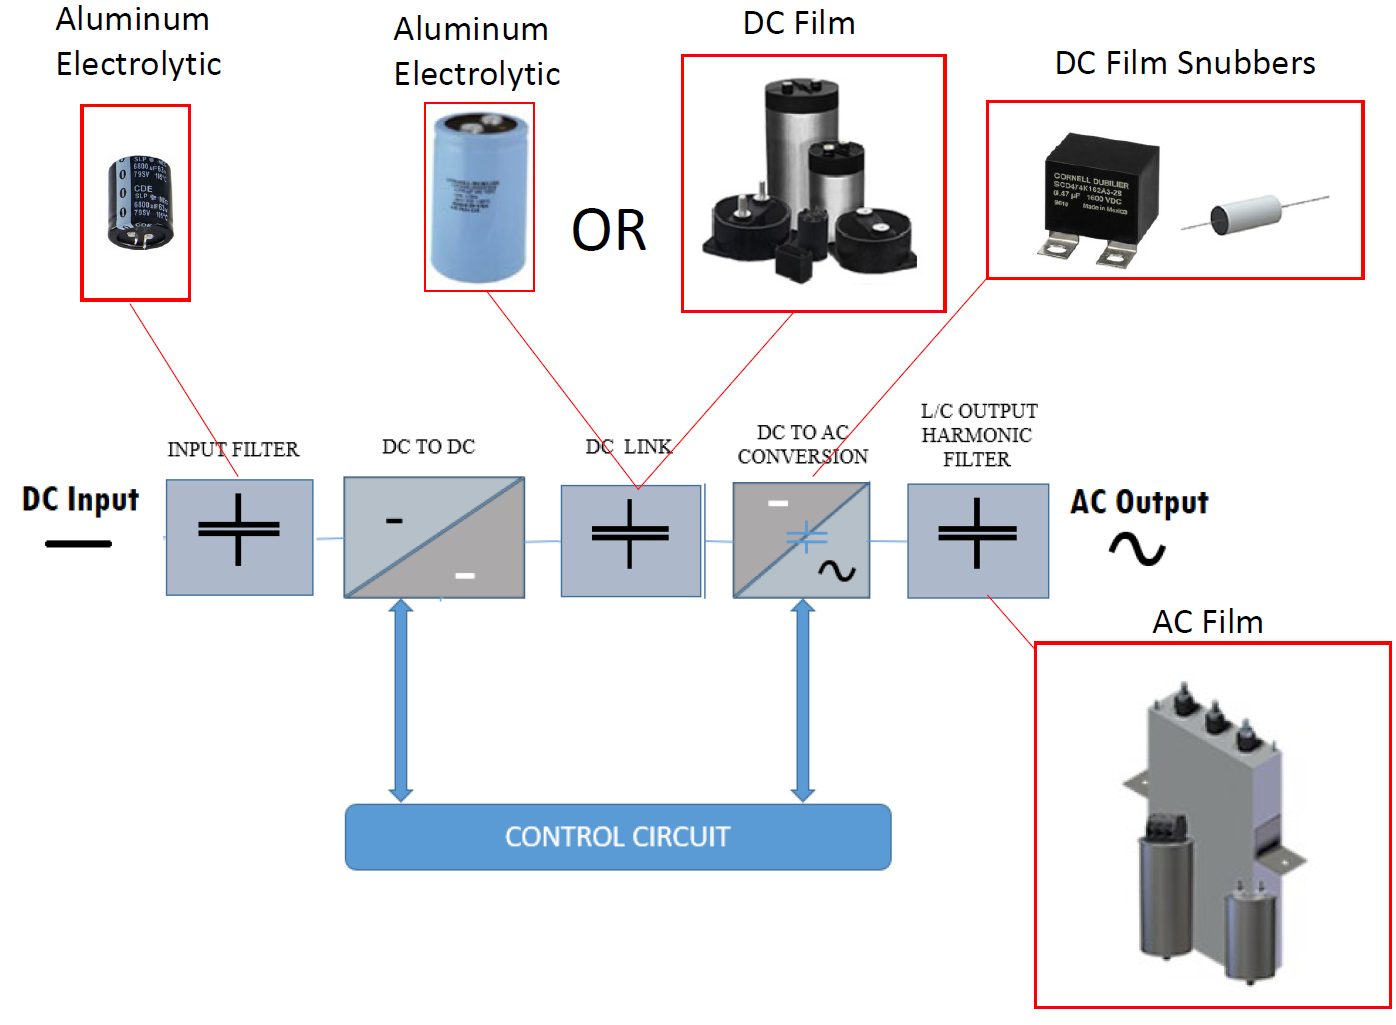
\includegraphics[width=\linewidth]{fig/lec08/capacitors_types.png}
    \caption{Typical capacitor locations in inverter and converter systems: input filter, DC-link, snubber, and AC harmonic filter capacitors. Adapted from Cornell Dubilier, \textit{Capacitors for High Power Inverters and Converters}}
\end{figure}
\end{column}
\end{columns}

\end{frame}


%%%%%%%%%%%%%%%%%%%%%%%%%%%%%%%%%%%%%%%%%%%%%%%%%%%%%%%%%%%%%
%% Capacitors in converter system examples
%%%%%%%%%%%%%%%%%%%%%%%%%%%%%%%%%%%%%%%%%%%%%%%%%%%%%%%%%%%%%
\begin{frame}
\frametitle{Capacitors in Practical Converter Systems}

\begin{columns}
\begin{column}{0.56\textwidth}
The same capacitor principles appear repeatedly in different converter systems.
\begin{itemize}
    \item \textbf{Fast DC EV charger:}
    \begin{itemize}
        \item AC input filter capacitor,
        \item DC-link capacitor,
        \item DC output filter capacitor.
    \end{itemize}

    \item \textbf{Solar inverter:}
    \begin{itemize}
        \item PV-side input filter,
        \item DC-link energy buffer,
        \item AC-side harmonic filter.
    \end{itemize}

    \item \textbf{UPS and VFD systems:}
    \begin{itemize}
        \item rectifier-side filtering,
        \item intermediate DC-link storage,
        \item inverter output filtering.
    \end{itemize}
\end{itemize}
\end{column}

\begin{column}{0.40\textwidth}
\begin{figure}
    \centering
    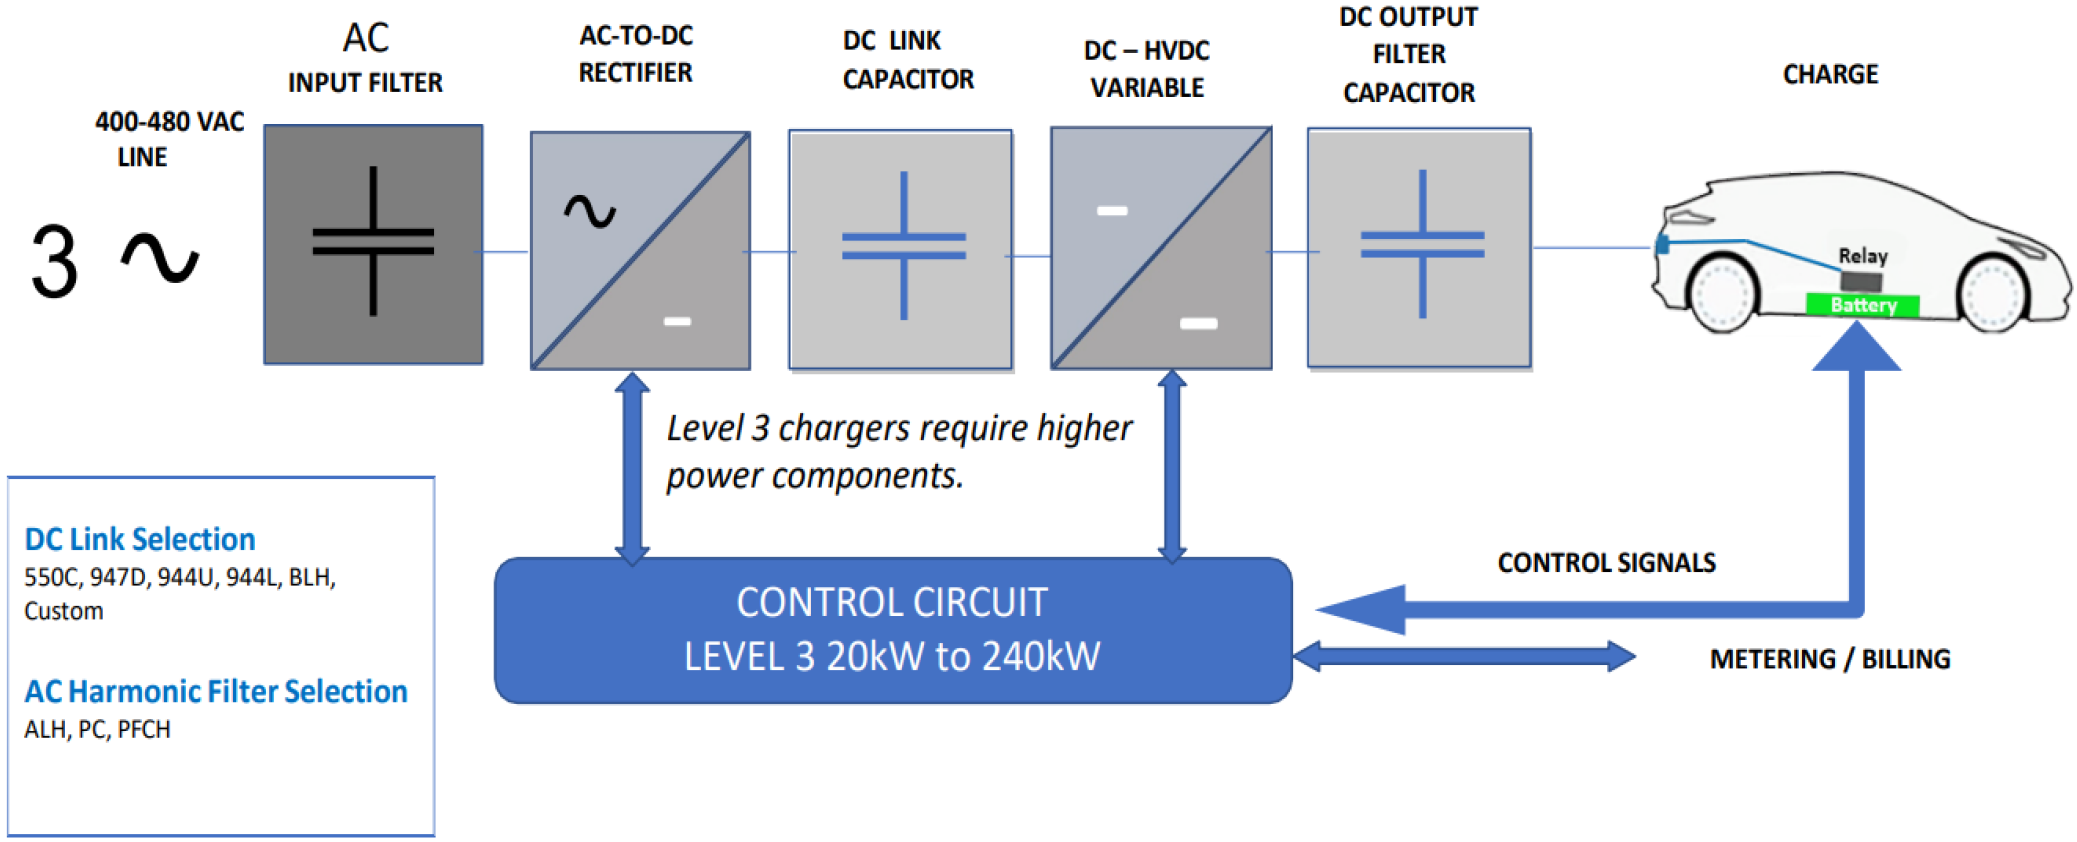
\includegraphics[width=\linewidth]{fig/lec08/fast_dc_ev_charger.png}
    \caption{Capacitor positions in a level-3 fast DC EV charger. Adapted from Cornell Dubilier, \textit{Capacitors for High Power Inverters and Converters}}
\end{figure}
\end{column}
\end{columns}
The capacitor technology changes with the location: electrolytic or film for energy storage, film for DC-link and snubber duties, and ceramics for high-frequency decoupling.
\end{frame}


%%%%%%%%%%%%%%%%%%%%%%%%%%%%%%%%%%%%%%%%%%%%%%%%%%%%%%%%%%%%%
%% Capacitor vs inductor
%%%%%%%%%%%%%%%%%%%%%%%%%%%%%%%%%%%%%%%%%%%%%%%%%%%%%%%%%%%%%
\begin{frame}
\frametitle{Capacitor versus Inductor: Electric-Field and Magnetic-Field Storage}

\begin{columns}
\begin{column}{0.55\textwidth}
A capacitor is the electrical dual of an inductor.
\begin{itemize}
    \item An inductor stores energy in a \textbf{magnetic field}.
    \item A capacitor stores energy in an \textbf{electric field}.
    \item An inductor resists a change in current:
    \begin{align}
        v_L = L\frac{di_L}{dt}
    \end{align}
    \item A capacitor resists a change in voltage:
    \begin{align}
        i_C = C\frac{dv_C}{dt}
    \end{align}
\end{itemize}
This is why inductors smooth current, whereas capacitors smooth voltage.
\end{column}

\begin{column}{0.41\textwidth}
\begin{center}
\begin{circuitikz}[scale=0.85, transform shape]
    \draw (0,0) to[L,l=$L$] (2,0);
    \node at (1,-0.7) {\small magnetic-field storage};
    \draw[->, thick] (-0.2,0.35) -- (0.5,0.35);
    \node at (0.2,0.65) {\small $i_L$};

    \draw (0,-2.0) to[C,l=$C$] (2,-2.0);
    \node at (1,-2.7) {\small electric-field storage};
    \draw[->, thick] (-0.2,-1.65) -- (0.5,-1.65);
    \node at (0.2,-1.35) {\small $i_C$};
\end{circuitikz}
\end{center}

\vspace{0.15cm}

\begin{block}{Power Electronics Interpretation}
\small
The inductor controls the current trajectory; the capacitor controls the voltage trajectory. Converter dynamics are largely shaped by the interaction of both.
\end{block}
\end{column}
\end{columns}

\end{frame}


%%%%%%%%%%%%%%%%%%%%%%%%%%%%%%%%%%%%%%%%%%%%%%%%%%%%%%%%%%%%%
%% Capacitor design questions
%%%%%%%%%%%%%%%%%%%%%%%%%%%%%%%%%%%%%%%%%%%%%%%%%%%%%%%%%%%%%
\begin{frame}
\frametitle{Capacitor Design Questions}
Before selecting a capacitor, the designer must identify the electrical, thermal, mechanical, and reliability requirements.
\begin{columns}
\begin{column}{0.56\textwidth}
\begin{itemize}
    \item What is the required capacitance?
    \item What is the maximum DC voltage?
    \item What ripple voltage is allowed?
    \item What RMS ripple current flows through the capacitor?
    \item What peak current or $dv/dt$ stress occurs during switching?
    \item What ESR and ESL are acceptable?
    \item What temperature rise is acceptable?
    \item What lifetime is required?
    \item Is the capacitor used for DC-link, snubber, EMI, resonant, or output filtering?
\end{itemize}

\end{column}

\begin{column}{0.40\textwidth}
\begin{block}{Selection Principle}
\small
A capacitor is not selected by capacitance alone. In power electronics, the correct capacitor is selected by a combined requirement:
\[
V,\; C,\; I_{\mathrm{rms}},\; I_{\mathrm{pk}},\; ESR,\; ESL,\; T,\; L_{\mathrm{life}}
\]
\end{block}

\begin{block}{Practical Source}
\small
The selection guide for capacitors should be structured based on voltage, capacitance, current withstand, and power-loss/temperature-rise checks.
\end{block}
\end{column}
\end{columns}

\end{frame}


%%%%%%%%%%%%%%%%%%%%%%%%%%%%%%%%%%%%%%%%%%%%%%%%%%%%%%%%%%%%%
%% Capacitance definition
%%%%%%%%%%%%%%%%%%%%%%%%%%%%%%%%%%%%%%%%%%%%%%%%%%%%%%%%%%%%%
\begin{frame}
\frametitle{Capacitance: Ability to Store Electric Charge}

\begin{columns}
\begin{column}{0.55\textwidth}
Capacitance describes how much electric charge is stored per unit voltage $C = \frac{Q}{V}$, where
\begin{itemize}
    \item $C$ is capacitance in farads,
    \item $Q$ is stored charge in coulombs,
    \item $V$ is voltage across the capacitor.
\end{itemize}
The current through a capacitor follows from differentiating charge:
\begin{align}
    i_C(t) = \frac{dQ}{dt}
           = C\frac{dv_C(t)}{dt}
\end{align}
Therefore, a capacitor conducts current only when its voltage changes. Under ideal steady-state DC conditions, capacitor current becomes zero.
\end{column}

\begin{column}{0.41\textwidth}
\begin{figure}
    \centering
    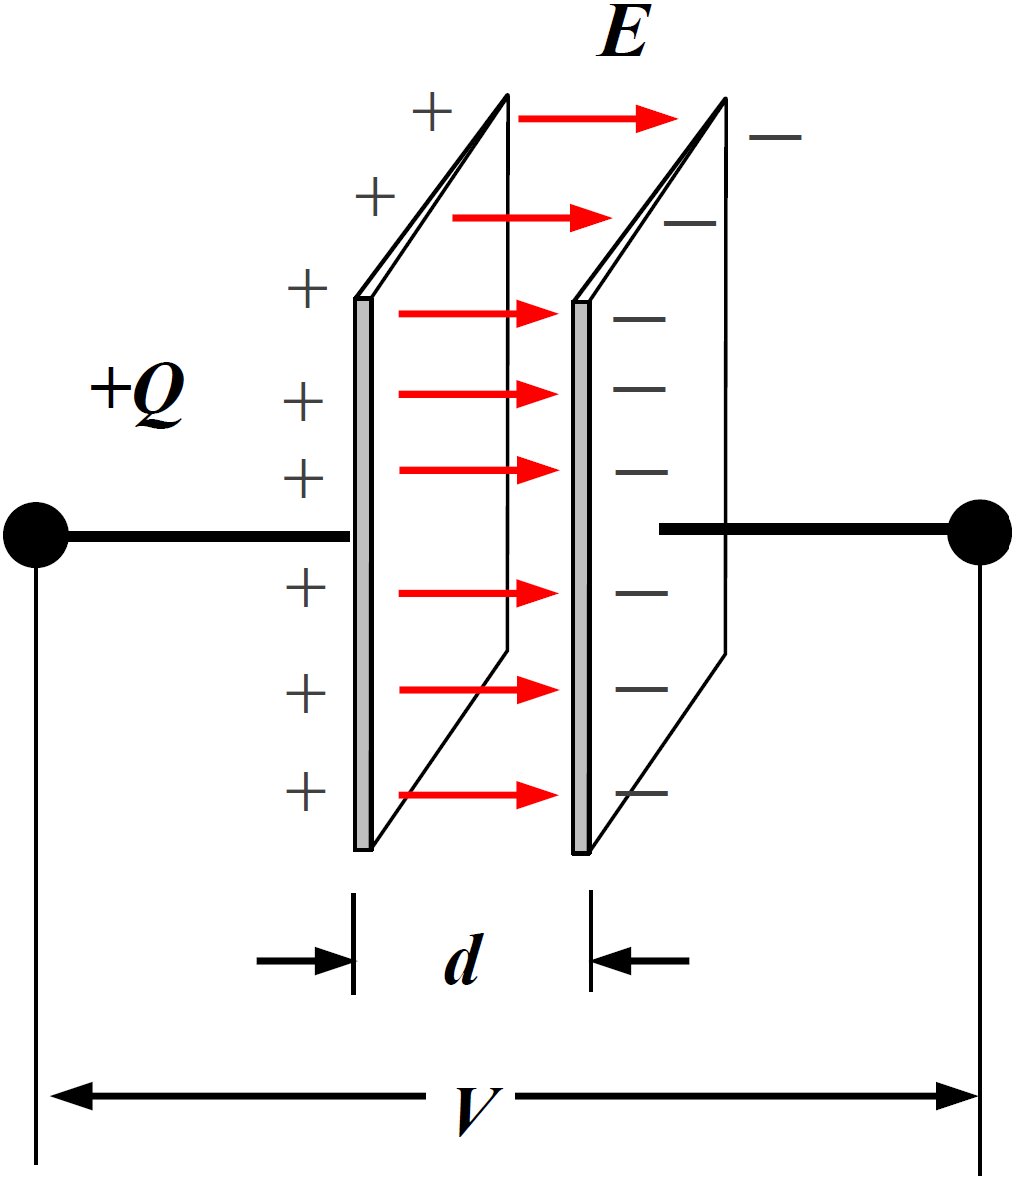
\includegraphics[width=0.6\linewidth]{fig/lec08/charge_and_electric_field.png}
    \caption{Electric charge and electric field strength between capacitor plates. Adapted from AIC tech, \textit{The Three Essential Characteristics of Capacitors}}
\end{figure}
\end{column}
\end{columns}

\end{frame}


%%%%%%%%%%%%%%%%%%%%%%%%%%%%%%%%%%%%%%%%%%%%%%%%%%%%%%%%%%%%%
%% Parallel plate capacitor
%%%%%%%%%%%%%%%%%%%%%%%%%%%%%%%%%%%%%%%%%%%%%%%%%%%%%%%%%%%%%
\begin{frame}
\frametitle{Parallel-Plate Capacitor}

\begin{columns}
\begin{column}{0.55\textwidth}
For an ideal parallel-plate capacitor,
\begin{align}
    C = \varepsilon_0\varepsilon_r \frac{A}{d}
\end{align}
where
\begin{itemize}
    \item $\varepsilon_0$ is the permittivity of free space,
    \item $\varepsilon_r$ is the relative permittivity of the dielectric,
    \item $A$ is the electrode area,
    \item $d$ is the dielectric thickness.
\end{itemize}
Hence three main ways to increase capacitance:
\begin{itemize}
    \item increase electrode area,
    \item use a dielectric with higher $\varepsilon_r$,
    \item reduce dielectric thickness.
\end{itemize}
\end{column}

\begin{column}{0.41\textwidth}
\begin{figure}
    \centering
    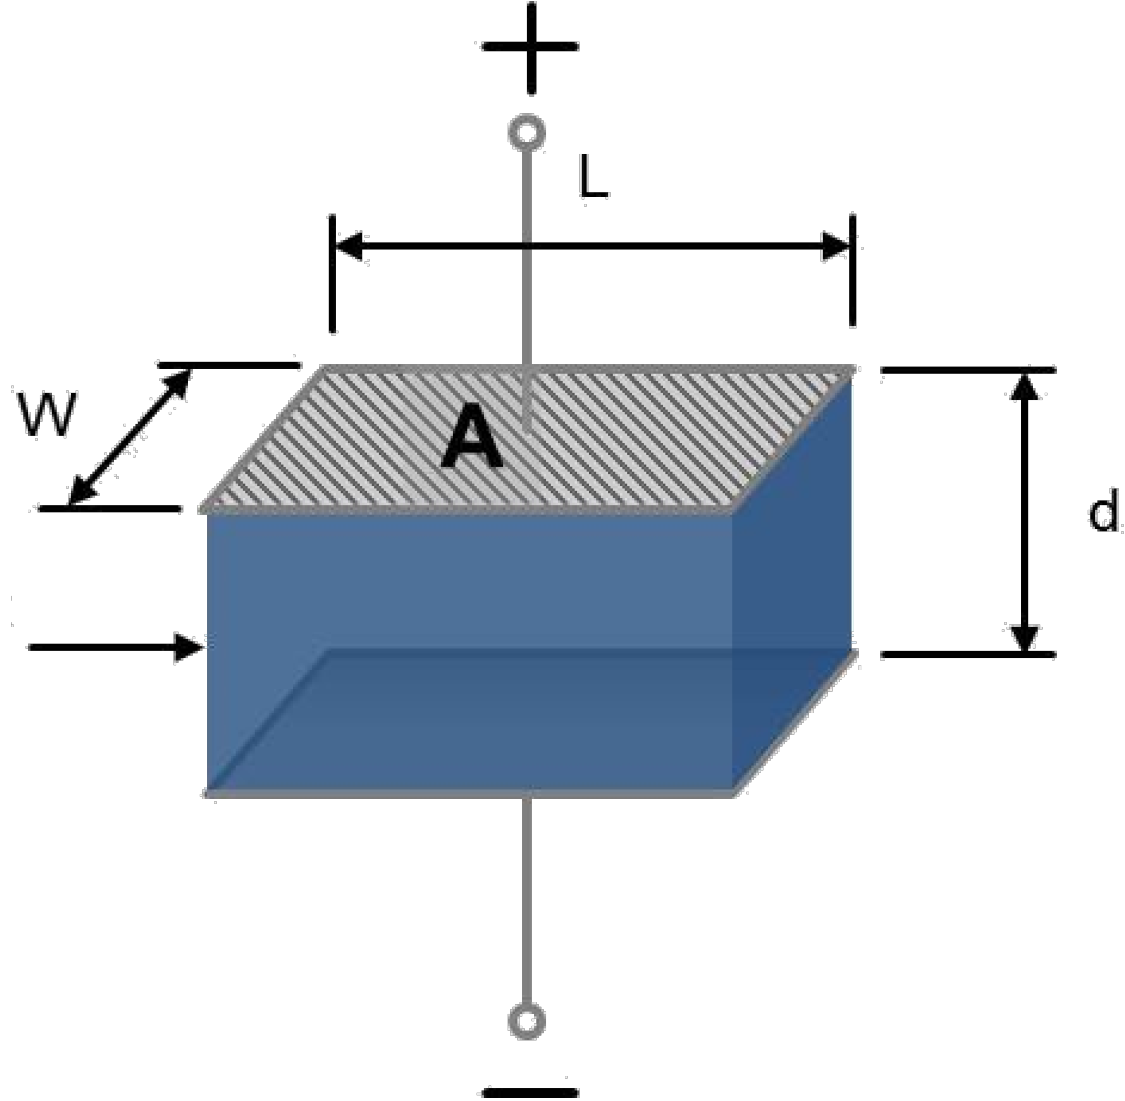
\includegraphics[width=0.6\linewidth]{fig/lec08/plate_capacitor.png}
    \caption{Construction of a plate capacitor and the relation $C=\varepsilon_0\varepsilon_r A/d$. Adapted from W{\"u}rth Elektronik, \textit{Fundamentals of Capacitor Technology and Their Applications}}
\end{figure}
\end{column}
\end{columns}
However, reducing $d$ increases the electric field stress and reduces voltage withstand capability.
\end{frame}


%%%%%%%%%%%%%%%%%%%%%%%%%%%%%%%%%%%%%%%%%%%%%%%%%%%%%%%%%%%%%
%% Electric field and dielectric stress
%%%%%%%%%%%%%%%%%%%%%%%%%%%%%%%%%%%%%%%%%%%%%%%%%%%%%%%%%%%%%
\begin{frame}
\frametitle{Electric Field and Dielectric Stress}

\begin{columns}
\begin{column}{0.56\textwidth}
The electric field inside a parallel-plate capacitor is approximately $E = \frac{V}{d}$, where $V$ is the applied voltage and $d$ is the dielectric thickness. This simple equation is extremely important for power electronics:
\begin{itemize}
    \item Higher voltage increases dielectric stress.
    \item Thinner dielectric increases capacitance but also increases electric field.
    \item Exceeding the dielectric strength causes partial discharge, insulation degradation, or breakdown.
    \item Voltage derating is therefore essential for long lifetime.
\end{itemize}
\end{column}

\begin{column}{0.40\textwidth}
    \vspace{-0.75cm}
\begin{block}{Design Interpretation}
The capacitance equation encourages small dielectric thickness, but the electric-field equation limits how small the dielectric can be:
\[
C \uparrow \quad \text{when} \quad d \downarrow
\]
\[
E \uparrow \quad \text{when} \quad d \downarrow
\]
\end{block}
\begin{block}{Practical Consequence}
Capacitor design is a compromise between capacitance density, voltage rating, loss, reliability, and lifetime.
\end{block}
\end{column}
\end{columns}
In real capacitors, field enhancement also occurs near electrode edges, metallization boundaries, terminals, and defects.
\end{frame}


%%%%%%%%%%%%%%%%%%%%%%%%%%%%%%%%%%%%%%%%%%%%%%%%%%%%%%%%%%%%%
%% Dielectric polarization
%%%%%%%%%%%%%%%%%%%%%%%%%%%%%%%%%%%%%%%%%%%%%%%%%%%%%%%%%%%%%
\begin{frame}
\frametitle{Dielectric Polarization}

\begin{columns}
\begin{column}{0.55\textwidth}
A dielectric is an insulating material that becomes polarized when exposed to an electric field.
When the dielectric is inserted between the plates:
\begin{itemize}
    \item bound charges shift slightly inside the material,
    \item an induced electric field is created,
    \item the net electric field for a given charge is reduced,
    \item more charge can be stored at the same applied voltage.
\end{itemize}
The capacitance therefore increases by the relative permittivity:
\begin{align}
    C = \varepsilon_r C_0
\end{align}
where $C_0$ is the capacitance without the dielectric.
\end{column}

\begin{column}{0.41\textwidth}
\begin{figure}
    \centering
    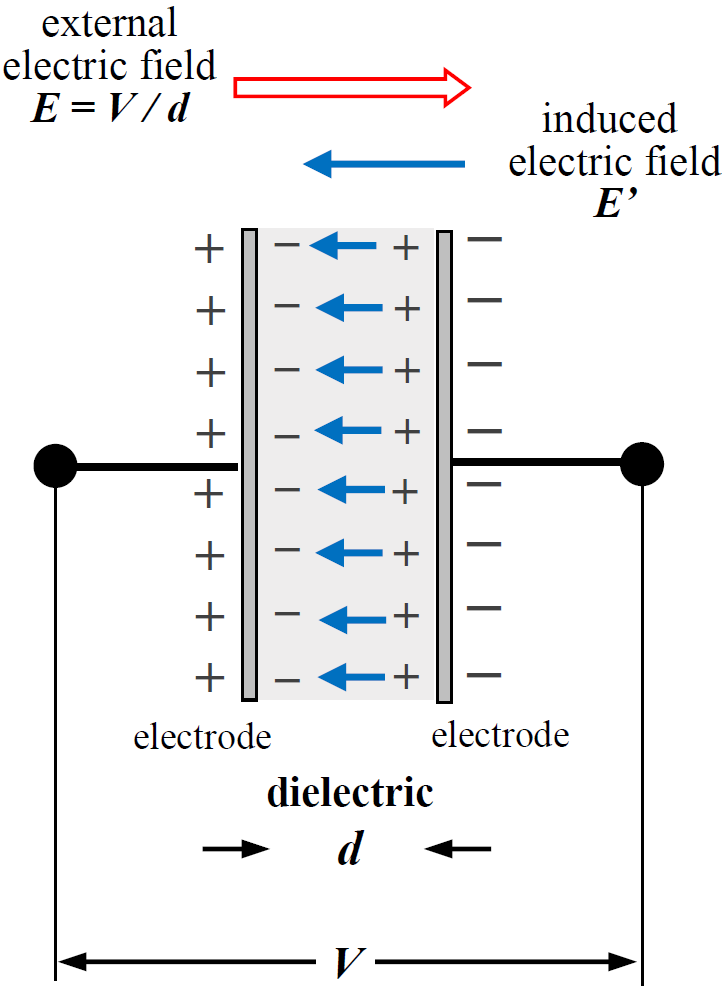
\includegraphics[width=0.5\linewidth]{fig/lec08/dielectric_polarization.png}
    \caption{Dielectric polarization caused by an applied electric field. Adapted from AIC tech, \textit{The Three Essential Characteristics of Capacitors}}
\end{figure}
\end{column}
\end{columns}
Different capacitor technologies are largely distinguished by their dielectric material.
\end{frame}


%%%%%%%%%%%%%%%%%%%%%%%%%%%%%%%%%%%%%%%%%%%%%%%%%%%%%%%%%%%%%
%% Dielectric materials
%%%%%%%%%%%%%%%%%%%%%%%%%%%%%%%%%%%%%%%%%%%%%%%%%%%%%%%%%%%%%
\begin{frame}
\frametitle{Dielectric Materials and Relative Permittivity}

\begin{columns}
\begin{column}{0.56\textwidth}
The dielectric determines capacitance density, loss, temperature stability, voltage dependence, and ageing. Typical examples:
\begin{itemize}
    \item \textbf{Polypropylene:} low loss, stable, widely used in film capacitors.
    \item \textbf{Aluminum oxide:} dielectric of aluminum electrolytic capacitors.
    \item \textbf{Tantalum oxide:} used in tantalum electrolytic capacitors.
    \item \textbf{Class 1 ceramics:} stable, low loss, lower capacitance.
    \item \textbf{Class 2 ceramics:} high capacitance, but voltage- and temperature-dependent.
\end{itemize}

\end{column}

\begin{column}{0.40\textwidth}
\begin{figure}
    \centering
    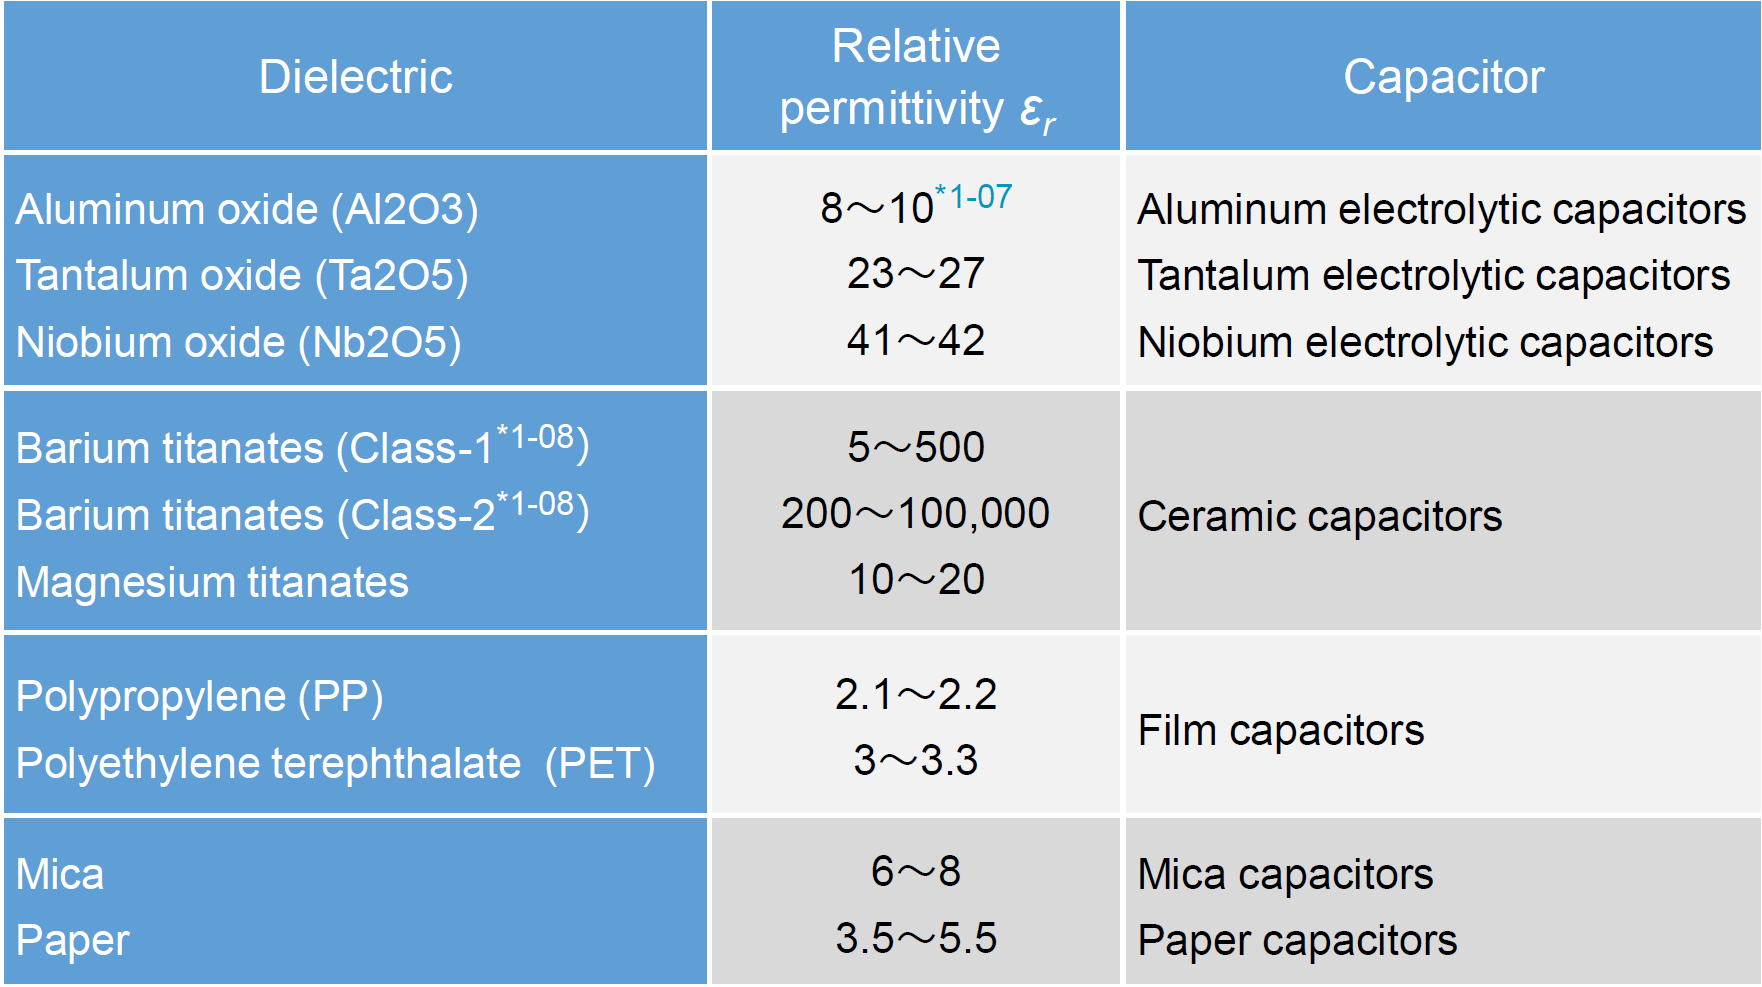
\includegraphics[width=\linewidth]{fig/lec08/dielectrics.png}
    \caption{Dielectric types, relative permittivity, and corresponding capacitor families. Adapted from AIC tech, \textit{The Three Essential Characteristics of Capacitors}}
\end{figure}
\end{column}
\end{columns}
High $\varepsilon_r$ gives high capacitance density, but not necessarily the best power-electronics capacitor. Loss, voltage dependence, ripple current, and thermal behaviour must also be considered.
\end{frame}


%%%%%%%%%%%%%%%%%%%%%%%%%%%%%%%%%%%%%%%%%%%%%%%%%%%%%%%%%%%%%
%% Stored energy
%%%%%%%%%%%%%%%%%%%%%%%%%%%%%%%%%%%%%%%%%%%%%%%%%%%%%%%%%%%%%
\begin{frame}
\frametitle{Energy Stored in a Capacitor}

\begin{columns}
\begin{column}{0.56\textwidth}
The energy stored in a capacitor is
\begin{align}
    E_C = \int_0^Q v\,dq
\end{align}
\begin{align}
    E_C = \frac{1}{2}CV^2 [\text{using} q = Cv]
\end{align}
Important observations:
\begin{itemize}
    \item Stored energy increases linearly with capacitance.
    \item Stored energy increases with the square of voltage.
    \item High-voltage DC-link capacitors can store dangerous energy even after the converter is switched off.
    \item Discharge resistors and safe handling procedures are therefore essential.
\end{itemize}

\end{column}

\begin{column}{0.40\textwidth}
\begin{figure}
    \centering
    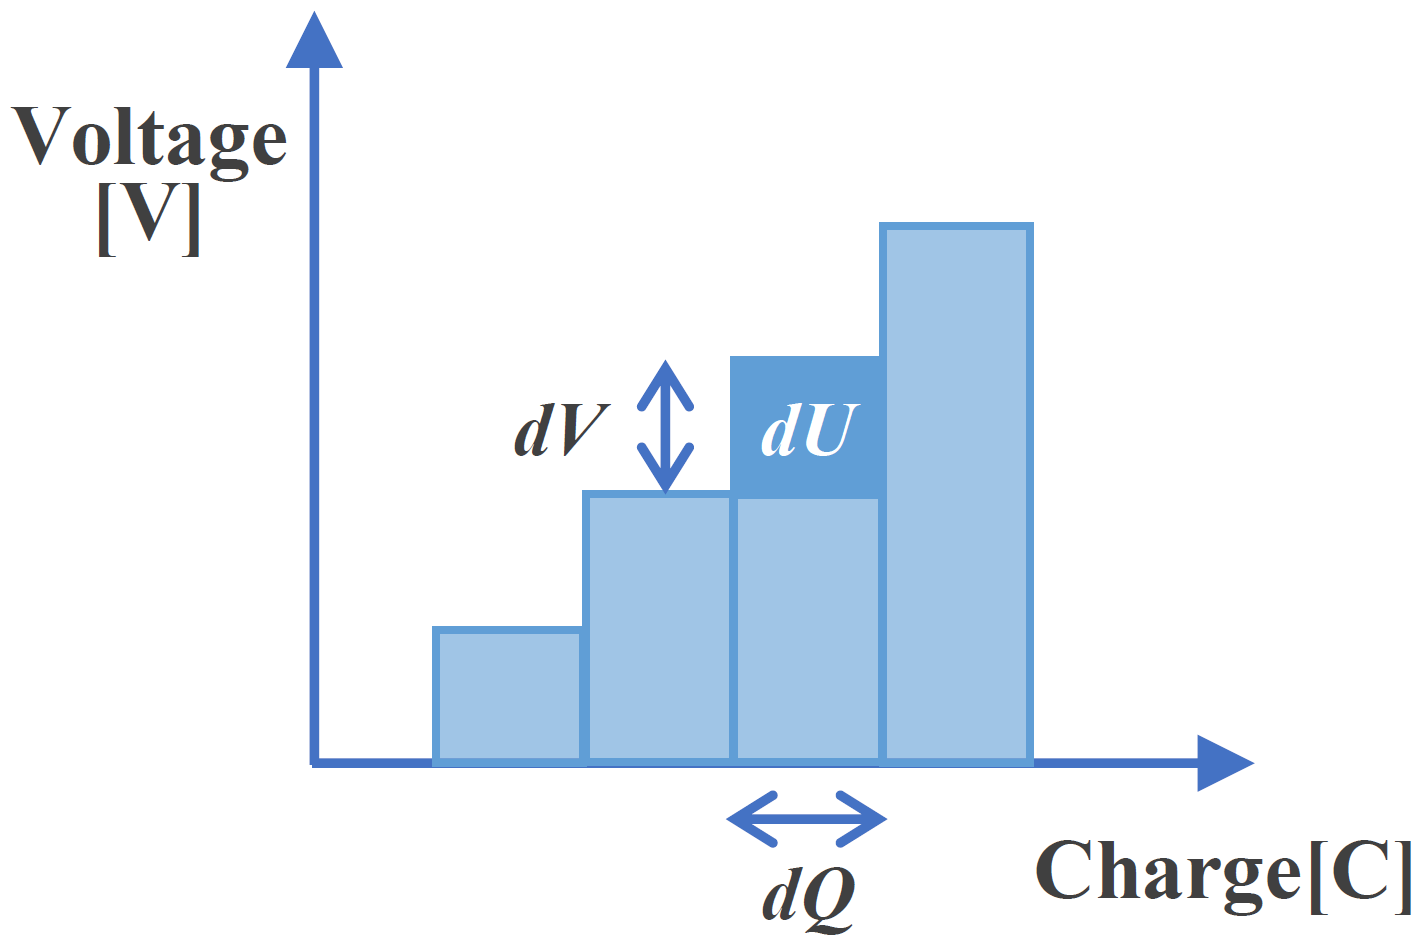
\includegraphics[width=0.5\linewidth]{fig/lec08/cap_energy_storage.png}
    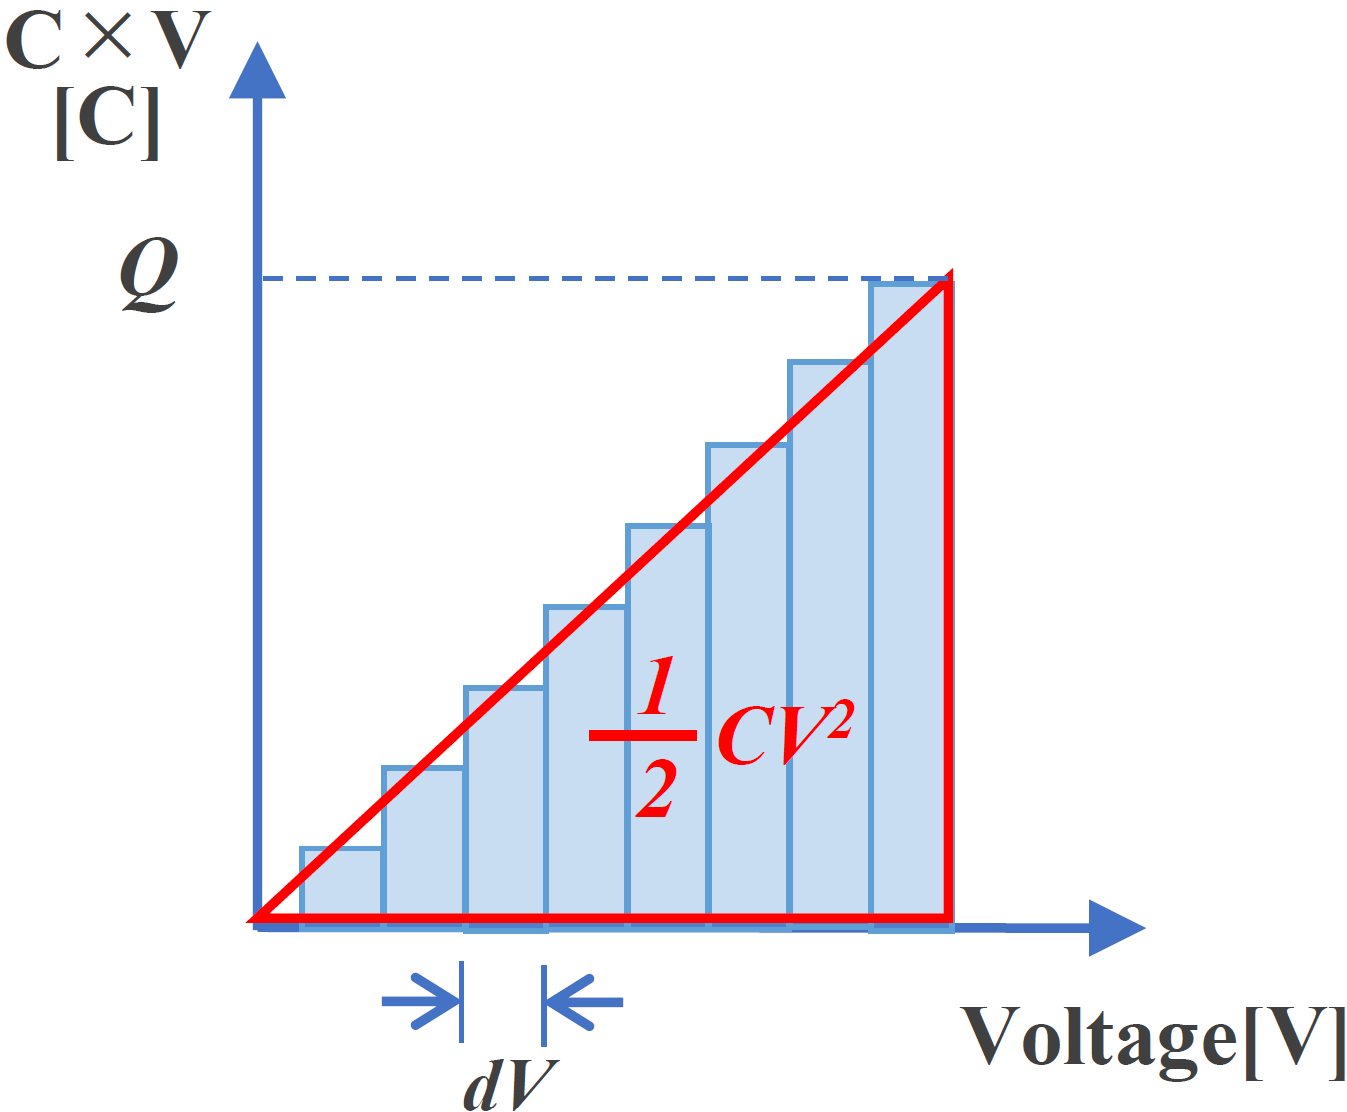
\includegraphics[width=0.5\linewidth]{fig/lec08/cap_energy_storage2.png}
    \caption{Charge--voltage relation and stored energy in a capacitor. Adapted from AIC tech, \textit{The Three Essential Characteristics of Capacitors}}
\end{figure}
\end{column}
\end{columns}
\end{frame}


%%%%%%%%%%%%%%%%%%%%%%%%%%%%%%%%%%%%%%%%%%%%%%%%%%%%%%%%%%%%%
%% Capacitor current and dvdt
%%%%%%%%%%%%%%%%%%%%%%%%%%%%%%%%%%%%%%%%%%%%%%%%%%%%%%%%%%%%%
\begin{frame}
\frametitle{Capacitor Current and $dv/dt$ Stress}

\begin{columns}
\begin{column}{0.55\textwidth}
The capacitor current is $i_C(t)=C\frac{dv_C(t)}{dt}$. This equation is central in switched-mode power converters.
\begin{itemize}
    \item A slowly varying voltage produces small capacitor current.
    \item A fast switching edge produces large current.
    \item High $dv/dt$ creates high peak current stress.
    \item In snubbers and DC-link decoupling, the capacitor must withstand repetitive high-current pulses.
\end{itemize}
For a linear voltage transition,
\begin{align}
    I_{\mathrm{pk}} = C\frac{\Delta V}{\Delta t}
\end{align}
\end{column}

\begin{column}{0.41\textwidth}
\begin{center}
\begin{circuitikz}[scale=0.80, transform shape]
    \draw (0,0) to[C,l=$C$] (0,-2);
    \draw (-1,0) -- (1,0);
    \draw (-1,-2) -- (1,-2);
    \draw[->, thick] (1.2,-1.7) -- (1.2,-0.3);
    \node at (1.55,-1.0) {$i_C$};

    \draw[->] (-0.6,-2.6) -- (2.8,-2.6);
    \draw[->] (-0.6,-2.6) -- (-0.6,-0.6);
    \draw[thick] (-0.4,-2.4) -- (0.5,-2.4) -- (2.1,-1.0) -- (2.6,-1.0);
    \node at (2.65,-2.75) {\small $t$};
    \node at (-0.95,-0.8) {\small $v_C$};
    \node at (1.3,-1.9) {\small $\Delta V/\Delta t$};
\end{circuitikz}
\end{center}

\begin{block}{Power Electronics Interpretation}
\small
Fast SiC/GaN switching increases $dv/dt$, so the capacitor must be evaluated for peak current, RMS current, ESL, mounting inductance, and thermal stress.
\end{block}
\end{column}
\end{columns}
Thus, increasing capacitance or reducing rise time increases pulse current.
\end{frame}


%%%%%%%%%%%%%%%%%%%%%%%%%%%%%%%%%%%%%%%%%%%%%%%%%%%%%%%%%%%%%
%% Charging and discharging
%%%%%%%%%%%%%%%%%%%%%%%%%%%%%%%%%%%%%%%%%%%%%%%%%%%%%%%%%%%%%
\begin{frame}
\frametitle{Charging and Discharging of a Capacitor}

\begin{columns}
\begin{column}{0.65\textwidth}
In RC charging circuit, the capacitor voltage rises exponentially:
\begin{align}
    v_C(t)=V\left(1-e^{-t/RC}\right)
\end{align}
The charging current is
\begin{align}
    i_C(t)=\frac{V}{R}e^{-t/RC}
\end{align}
The time constant is $\tau = RC$. In power electronics, this principle appears in:
\begin{itemize}
    \item DC-link pre-charge circuits,
    \item discharge resistors,
    \item soft-start circuits,
    \item hold-up time design, and safety after shutdown.
\end{itemize}
\end{column}

\begin{column}{0.35\textwidth}
\begin{figure}
    \centering
    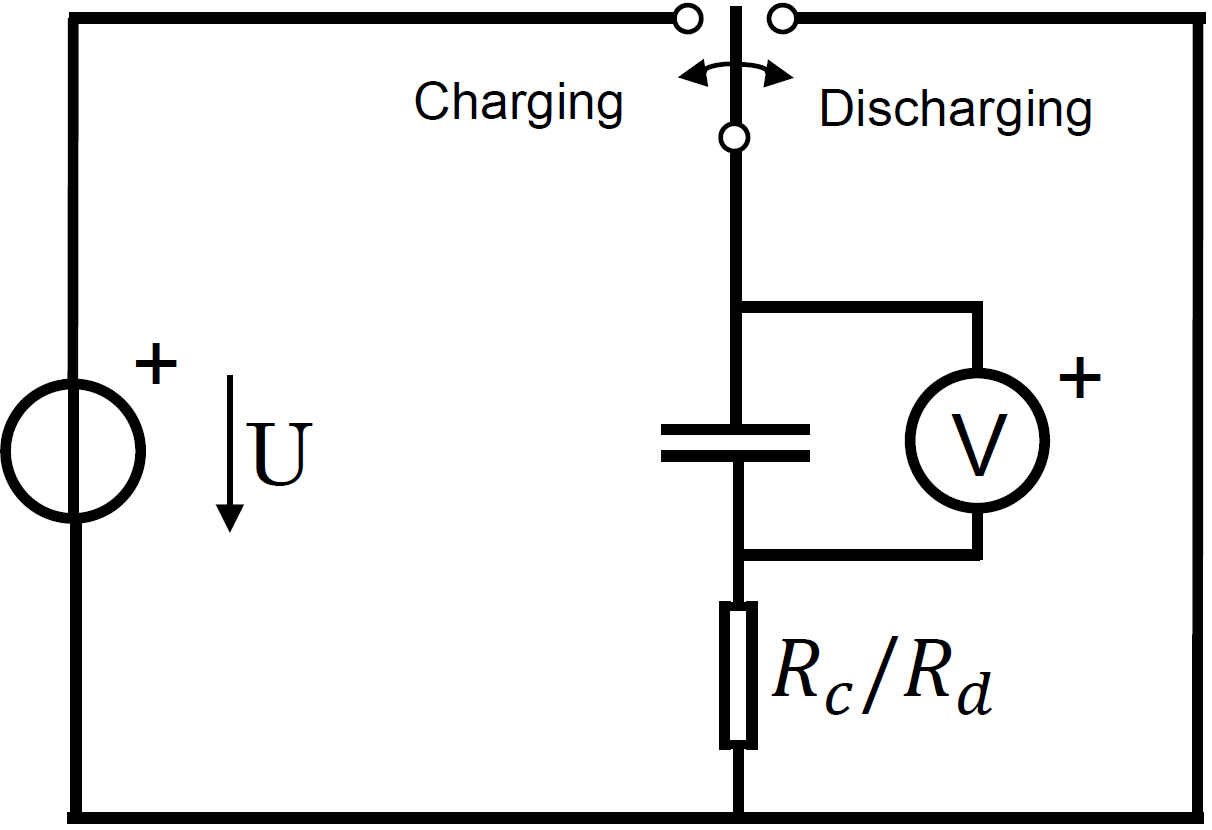
\includegraphics[width=0.8\linewidth]{fig/lec08/charging_discharging.png}
    \caption{Charging and discharging waveforms of a capacitor with time constant $\tau=RC$. Adapted from W{\"u}rth Elektronik, \textit{Fundamentals of Capacitor Technology and Their Applications}}
\end{figure}
\end{column}
\end{columns}

\end{frame}


%%%%%%%%%%%%%%%%%%%%%%%%%%%%%%%%%%%%%%%%%%%%%%%%%%%%%%%%%%%%%
%% Capacitive reactance
%%%%%%%%%%%%%%%%%%%%%%%%%%%%%%%%%%%%%%%%%%%%%%%%%%%%%%%%%%%%%
\begin{frame}
\frametitle{Capacitor in AC Circuits: Capacitive Reactance}
\begin{columns}
\begin{column}{0.56\textwidth}
For sinusoidal excitation, the impedance of an ideal capacitor is $Z_C = \frac{1}{j\omega C}$, and the capacitive reactance magnitude is
\begin{align}
    X_C = \frac{1}{\omega C}
        = \frac{1}{2\pi f C}
\end{align}
Therefore:
\begin{itemize}
    \item at low frequency, $X_C$ is large,
    \item at high frequency, $X_C$ becomes small,
    \item capacitor current leads capacitor voltage by $90^\circ$ in the ideal case,
    \item capacitors can be used for filtering, bypassing, coupling, and resonance.
\end{itemize}
\end{column}

\begin{column}{0.40\textwidth}
\begin{center}
\begin{circuitikz}[scale=0.80, transform shape]
    \draw (0,0) to[sV,l=$v_C$] (0,-2)
          to[C,l=$C$] (2,-2)
          -- (2,0) -- (0,0);

    \draw[->, thick] (3.0,-1.2) -- (4.2,-1.2);
    \node at (4.4,-1.2) {$V_C$};

    \draw[->, thick] (3.0,-1.2) -- (3.0,0.0);
    \node at (3.0,0.25) {$I_C$};

    \node at (3.75,-0.5) {\small $I_C$ leads $V_C$};
\end{circuitikz}
\end{center}
\begin{block}{Design Message}
\small
Capacitors are selected by their impedance over the relevant frequency range, not only by their nominal capacitance.
\end{block}
\end{column}
\end{columns}
However, real capacitors stop behaving ideally at high frequency due to ESR and ESL.
\end{frame}


%%%%%%%%%%%%%%%%%%%%%%%%%%%%%%%%%%%%%%%%%%%%%%%%%%%%%%%%%%%%%
%% Ideal capacitor summary
%%%%%%%%%%%%%%%%%%%%%%%%%%%%%%%%%%%%%%%%%%%%%%%%%%%%%%%%%%%%%
\begin{frame}
\frametitle{Summary of Ideal Capacitor Behaviour}
\begin{itemize}
    \item A capacitor stores electric charge according to $Q=CV$.
    \item The capacitance of an ideal parallel-plate capacitor is
    \begin{align}
        C=\varepsilon_0\varepsilon_r\frac{A}{d}
    \end{align}
    \item The electric field stress is approximately
    \begin{align}
        E=\frac{V}{d}
    \end{align}
    \item The capacitor current is proportional to voltage slew rate:
    \begin{align}
        i_C=C\frac{dv_C}{dt}
    \end{align}
    \item The stored energy is
    \begin{align}
        E_C=\frac{1}{2}CV^2
    \end{align}
    \item In DC steady state, an ideal capacitor behaves as an open circuit.
    \item In AC and switching circuits, it provides a frequency-dependent current path.
\end{itemize}
\end{frame}


%%%%%%%%%%%%%%%%%%%%%%%%%%%%%%%%%%%%%%%%%%%%%%%%%%%%%%%%%%%%%
%% Why ideal capacitor model is not enough
%%%%%%%%%%%%%%%%%%%%%%%%%%%%%%%%%%%%%%%%%%%%%%%%%%%%%%%%%%%%%
\begin{frame}
\frametitle{Why is the Ideal Capacitor Model Not Enough?}
The ideal capacitor relation $i_C = C\frac{dv_C}{dt}$ is useful for understanding the basic function of a capacitor. However, it is not sufficient for practical power electronic converter design. A real capacitor also contains parasitic and loss elements:

\begin{itemize}
    \item \textbf{Equivalent series resistance (ESR):} produces heat under ripple current.
    \item \textbf{Equivalent series inductance (ESL):} causes high-frequency impedance rise and voltage spikes.
    \item \textbf{Leakage resistance:} allows a small DC current through the dielectric.
    \item \textbf{Dielectric loss:} produces additional AC loss, usually represented by $\tan\delta$.
    \item \textbf{Dielectric absorption:} causes residual or recovery voltage after discharge.
\end{itemize}

Therefore, in power electronics, a capacitor must be treated as a frequency-dependent impedance rather than as a fixed capacitance.

\end{frame}


%%%%%%%%%%%%%%%%%%%%%%%%%%%%%%%%%%%%%%%%%%%%%%%%%%%%%%%%%%%%%
%% Real capacitor equivalent circuit
%%%%%%%%%%%%%%%%%%%%%%%%%%%%%%%%%%%%%%%%%%%%%%%%%%%%%%%%%%%%%
\begin{frame}
\frametitle{Equivalent Circuit of a Real Capacitor}

\begin{columns}
\begin{column}{0.55\textwidth}
A practical capacitor can be represented by an ideal capacitance combined with parasitic resistance, inductance, and leakage paths.
\begin{itemize}
    \item $C$ represents the useful capacitance.
    \item $R_{\mathrm{ESR}}$ represents ohmic and dielectric losses.
    \item $L_{\mathrm{ESL}}$ represents terminal, lead, winding, and layout inductance.
    \item $R_{\mathrm{leak}}$ represents insulation resistance and DC leakage.
\end{itemize}
The simplified impedance is
\begin{align}
    Z(j\omega)
    =
    R_{\mathrm{ESR}}
    +
    j\omega L_{\mathrm{ESL}}
    +
    \frac{1}{j\omega C}
\end{align}
\end{column}
\begin{column}{0.41\textwidth}
\begin{center}
\begin{circuitikz}[scale=0.88, transform shape]
    \draw (0,0) to[L,l=$L_{\mathrm{ESL}}$] (1.7,0)
              to[R,l=$R_{\mathrm{ESR}}$] (3.4,0)
              to[C,l=$C$] (3.4,-2.0)
              -- (0,-2.0) -- (0,0);

    \draw (4.2,0) -- (4.2,-2.0);
    \draw (3.4,0) -- (4.2,0);
    \draw (3.4,-2.0) -- (4.2,-2.0);
    \draw (4.2,0) to[R,l=$R_{\mathrm{leak}}$] (4.2,-2.0);

    \node at (-0.25,-1.0) {$+$};
    \node at (-0.25,-1.35) {$-$};
\end{circuitikz}
\end{center}

\begin{block}{Model Interpretation}
The useful capacitance stores energy, but ESR, ESL, and leakage determine loss, heating, resonance, switching spikes, and long-term reliability.
\end{block}
\end{column}
\end{columns}
This expression already explains why the same capacitor behaves differently at low, medium, and high frequency.
\end{frame}


%%%%%%%%%%%%%%%%%%%%%%%%%%%%%%%%%%%%%%%%%%%%%%%%%%%%%%%%%%%%%
%% ESR
%%%%%%%%%%%%%%%%%%%%%%%%%%%%%%%%%%%%%%%%%%%%%%%%%%%%%%%%%%%%%
\begin{frame}
\frametitle{Equivalent Series Resistance: ESR}

\begin{columns}
\begin{column}{0.56\textwidth}
The equivalent series resistance represents all loss mechanisms that appear as an effective resistance in series with the capacitance. Main contributors include:
\begin{itemize}
    \item electrode resistance,
    \item metallization resistance,
    \item terminal and contact resistance,
    \item electrolyte resistance in electrolytic capacitors,
    \item dielectric losses under AC excitation.
\end{itemize}
The most important consequence of ESR is self-heating:
\begin{align}
    P_{\mathrm{ESR}}
    =
    I_{\mathrm{rms}}^2 R_{\mathrm{ESR}}
\end{align}
\end{column}

\begin{column}{0.40\textwidth}
\begin{figure}
    \centering
    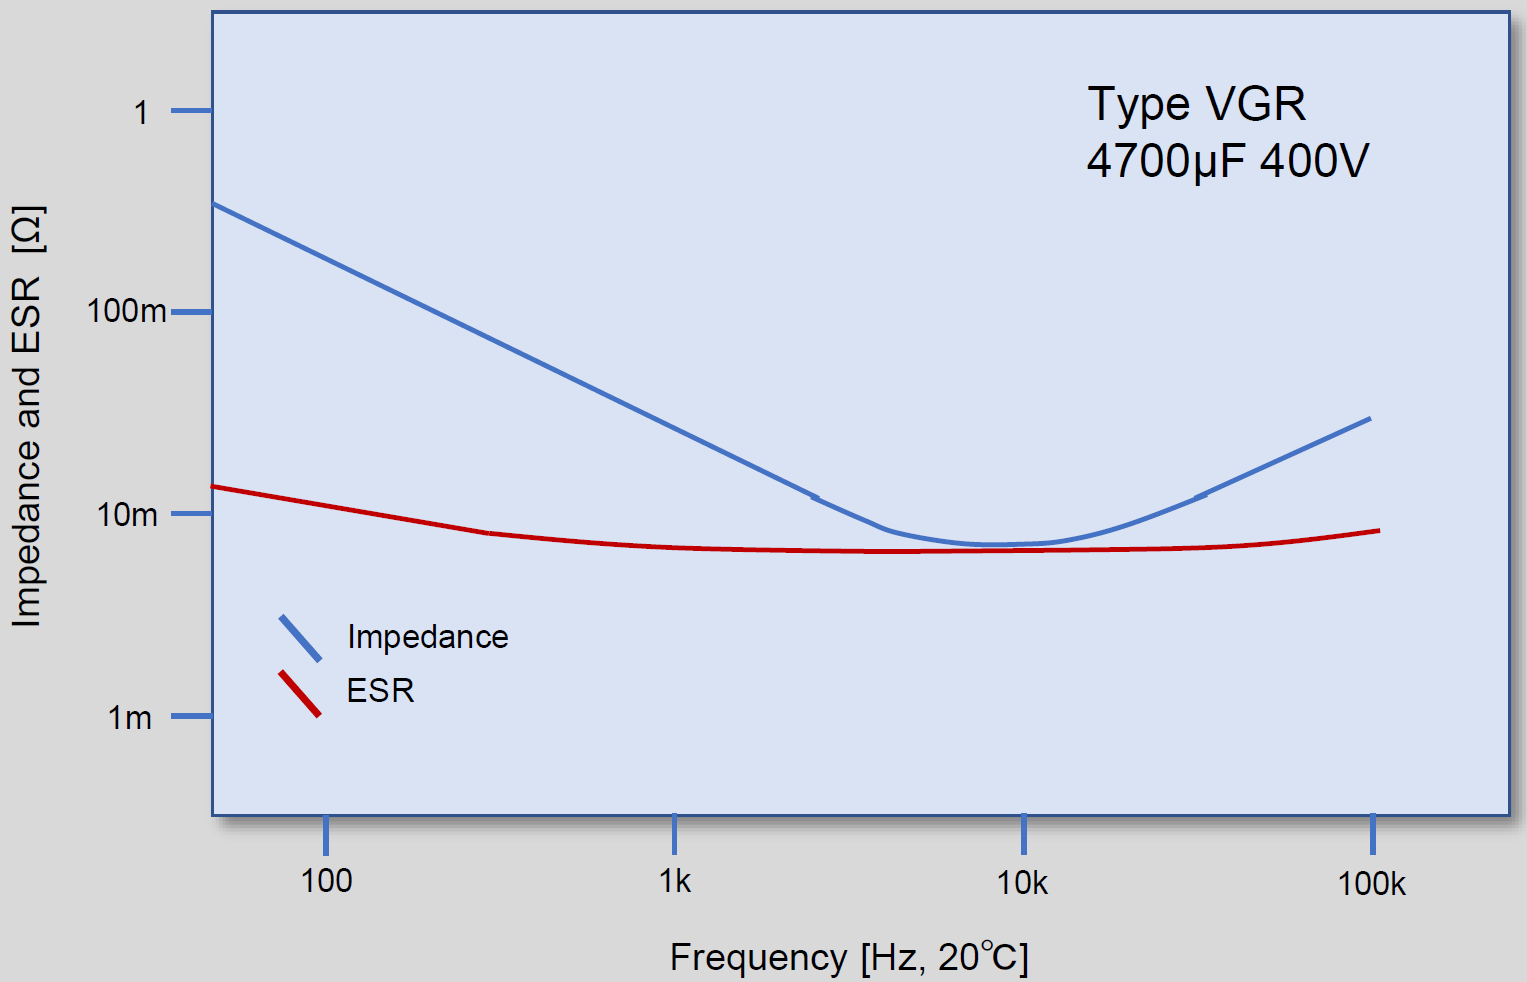
\includegraphics[width=0.8\linewidth]{fig/lec08/impedance_ESR_frequency.png}
    \caption{Impedance and ESR variation with frequency for an aluminum electrolytic capacitor. Adapted from AIC tech, \textit{The Three Essential Characteristics of Capacitors}}
\end{figure}
\end{column}
\end{columns}
A capacitor carrying high ripple current can fail thermally even when its voltage and capacitance ratings appear correct.
\end{frame}


%%%%%%%%%%%%%%%%%%%%%%%%%%%%%%%%%%%%%%%%%%%%%%%%%%%%%%%%%%%%%
%% ESR design implication
%%%%%%%%%%%%%%%%%%%%%%%%%%%%%%%%%%%%%%%%%%%%%%%%%%%%%%%%%%%%%
\begin{frame}
\frametitle{ESR: Design Consequences}
\begin{columns}
\begin{column}{0.5\textwidth}
ESR is critical in converter capacitors: it sets ripple voltage, loss, and lifetime. For a ripple current component,
\begin{align}
    \Delta v_{\mathrm{ESR}}
    =
    i_C R_{\mathrm{ESR}}
\end{align}
and the thermal loss is
\begin{align}
    P_{\mathrm{loss}}
    =
    I_{\mathrm{C,rms}}^2R_{\mathrm{ESR}}
\end{align}
High ESR causes:
\begin{itemize}
    \item larger ripple voltage,
    \item increased internal hot-spot temperature,
    \item accelerated ageing,
    \item reduced ripple-current capability,
    \item possible thermal runaway in severe cases.
\end{itemize}
\end{column}

\begin{column}{0.48\textwidth}
\begin{block}{Power Electronics Interpretation}
\small
In a DC-link or output capacitor, the RMS current rating is often more restrictive than the capacitance rating. A larger capacitance value does not automatically mean a better capacitor if ESR and thermal resistance are poor.
\end{block}
\begin{block}{Practical Check}
\small
Always check:
\[
I_{\mathrm{C,rms}} < I_{\mathrm{rated,rms}}
\]
at the expected operating temperature and cooling condition.
\end{block}
\end{column}
\end{columns}

\end{frame}


%%%%%%%%%%%%%%%%%%%%%%%%%%%%%%%%%%%%%%%%%%%%%%%%%%%%%%%%%%%%%
%% ESL
%%%%%%%%%%%%%%%%%%%%%%%%%%%%%%%%%%%%%%%%%%%%%%%%%%%%%%%%%%%%%
\begin{frame}
\frametitle{Equivalent Series Inductance: ESL}

\begin{columns}
\begin{column}{0.56\textwidth}
The equivalent series inductance is caused by the current path through terminals, leads, internal electrodes, tabs, windings, busbars, and PCB layout. At high frequency, $X_L = \omega L_{\mathrm{ESL}}$ becomes significant. ESL causes:
\begin{itemize}
    \item impedance increase above self-resonance,
    \item voltage overshoot during fast current commutation,
    \item reduced high-frequency decoupling effectiveness,
    \item increased switching-loop ringing,
    \item EMI problems in SiC and GaN converters.
\end{itemize}
The voltage generated by ESL is
\begin{align}
    v_{\mathrm{ESL}} = L_{\mathrm{ESL}}\frac{di}{dt}
\end{align}
\end{column}

\begin{column}{0.40\textwidth}
\begin{figure}
    \centering
    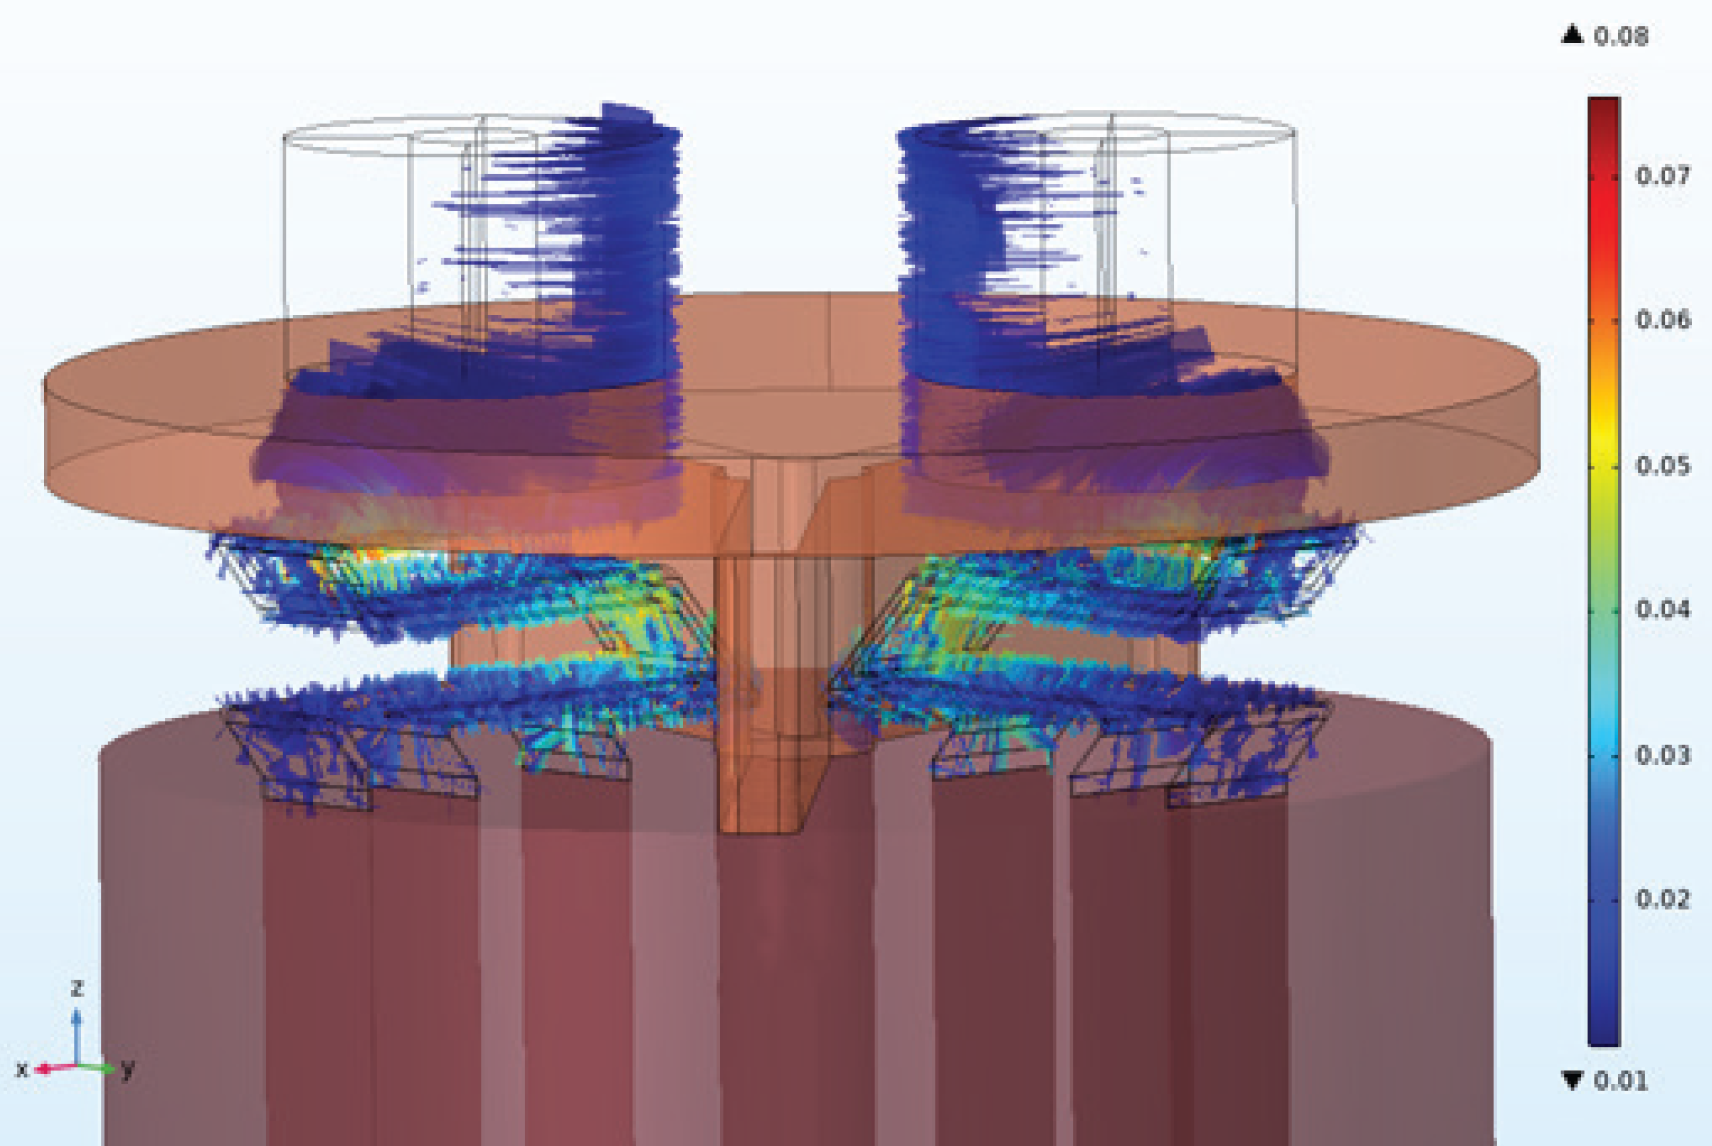
\includegraphics[width=0.8\linewidth]{fig/lec08/flux_lines_terminal_inductance.png}
    \caption{Typical magnetic flux lines in a screw-terminal capacitor with ripple current, illustrating terminal and tab loop inductance. Adapted from Knowles/Cornell Dubilier, \textit{Aluminum Electrolytic Capacitor Application Guide}}
\end{figure}
\end{column}
\end{columns}

\end{frame}


%%%%%%%%%%%%%%%%%%%%%%%%%%%%%%%%%%%%%%%%%%%%%%%%%%%%%%%%%%%%%
%% ESL and switching spikes
%%%%%%%%%%%%%%%%%%%%%%%%%%%%%%%%%%%%%%%%%%%%%%%%%%%%%%%%%%%%%
\begin{frame}
\frametitle{ESL and Switching Voltage Spikes}

\begin{columns}
\begin{column}{0.55\textwidth}
In fast-switching converters, the capacitor current can change within a few nanoseconds. The parasitic inductive voltage becomes
\begin{align}
    v_{\mathrm{spike}}
    =
    L_{\mathrm{loop}}
    \frac{di}{dt}
\end{align}
with $L_{\mathrm{loop}} =$ capacitor ESL + layout inductance. In SiC/GaN converters:
\begin{itemize}
    \item high $di/dt$,
    \item minimize loop area,
    \item use compact PCB loops or laminated busbars,
    \item add local HF ceramic/power-ceramic capacitors.
\end{itemize}
\end{column}

\begin{column}{0.41\textwidth}
\begin{center}
\begin{circuitikz}[scale=0.82, transform shape]
    \draw (0,0) to[V,l=$V_{\mathrm{dc}}$] (0,-2.5);
    \draw (0,0) -- (1.2,0)
          to[L,l=$L_{\mathrm{loop}}$] (2.7,0)
          to[C,l=$C_{\mathrm{dc}}$] (2.7,-2.5)
          -- (0,-2.5);

    \draw (2.7,0) -- (4.2,0)
          to[short] (4.2,-0.8)
          to[closing switch,l=$S$] (4.2,-1.7)
          to[short] (4.2,-2.5)
          -- (2.7,-2.5);

    \draw[->, thick] (1.3,0.45) -- (2.4,0.45);
    \node at (1.85,0.75) {\small $di/dt$};
    \node at (2.0,-3.0) {\small compact DC-link loop};
\end{circuitikz}
\end{center}

\begin{block}{Design Message}
For WBG converters, the capacitor and layout must be designed together. A low-ESL capacitor can still perform poorly if the external loop inductance is large.
\end{block}
\end{column}
\end{columns}

\end{frame}


%%%%%%%%%%%%%%%%%%%%%%%%%%%%%%%%%%%%%%%%%%%%%%%%%%%%%%%%%%%%%
%% Impedance versus frequency
%%%%%%%%%%%%%%%%%%%%%%%%%%%%%%%%%%%%%%%%%%%%%%%%%%%%%%%%%%%%%
\begin{frame}
\frametitle{Impedance versus Frequency}
\begin{columns}
\begin{column}{0.56\textwidth}
For the simplified series RLC capacitor model,
\begin{align}
    Z(j\omega)
    =
    R_{\mathrm{ESR}}
    +
    j\left(
    \omega L_{\mathrm{ESL}}
    -
    \frac{1}{\omega C}
    \right)
\end{align}
The magnitude becomes
\begin{align}
    |Z|
    =
    \sqrt{
    R_{\mathrm{ESR}}^2
    +
    \left(
    \omega L_{\mathrm{ESL}}
    -
    \frac{1}{\omega C}
    \right)^2
    }
\end{align}
Three regions are observed:
\begin{itemize}
    \item \textbf{Low frequency:} capacitive reactance dominates.
    \item \textbf{Near resonance:} impedance is close to ESR.
    \item \textbf{High frequency:} ESL dominates and the capacitor behaves inductively.
\end{itemize}
\end{column}

\begin{column}{0.40\textwidth}
\begin{figure}
    \centering
    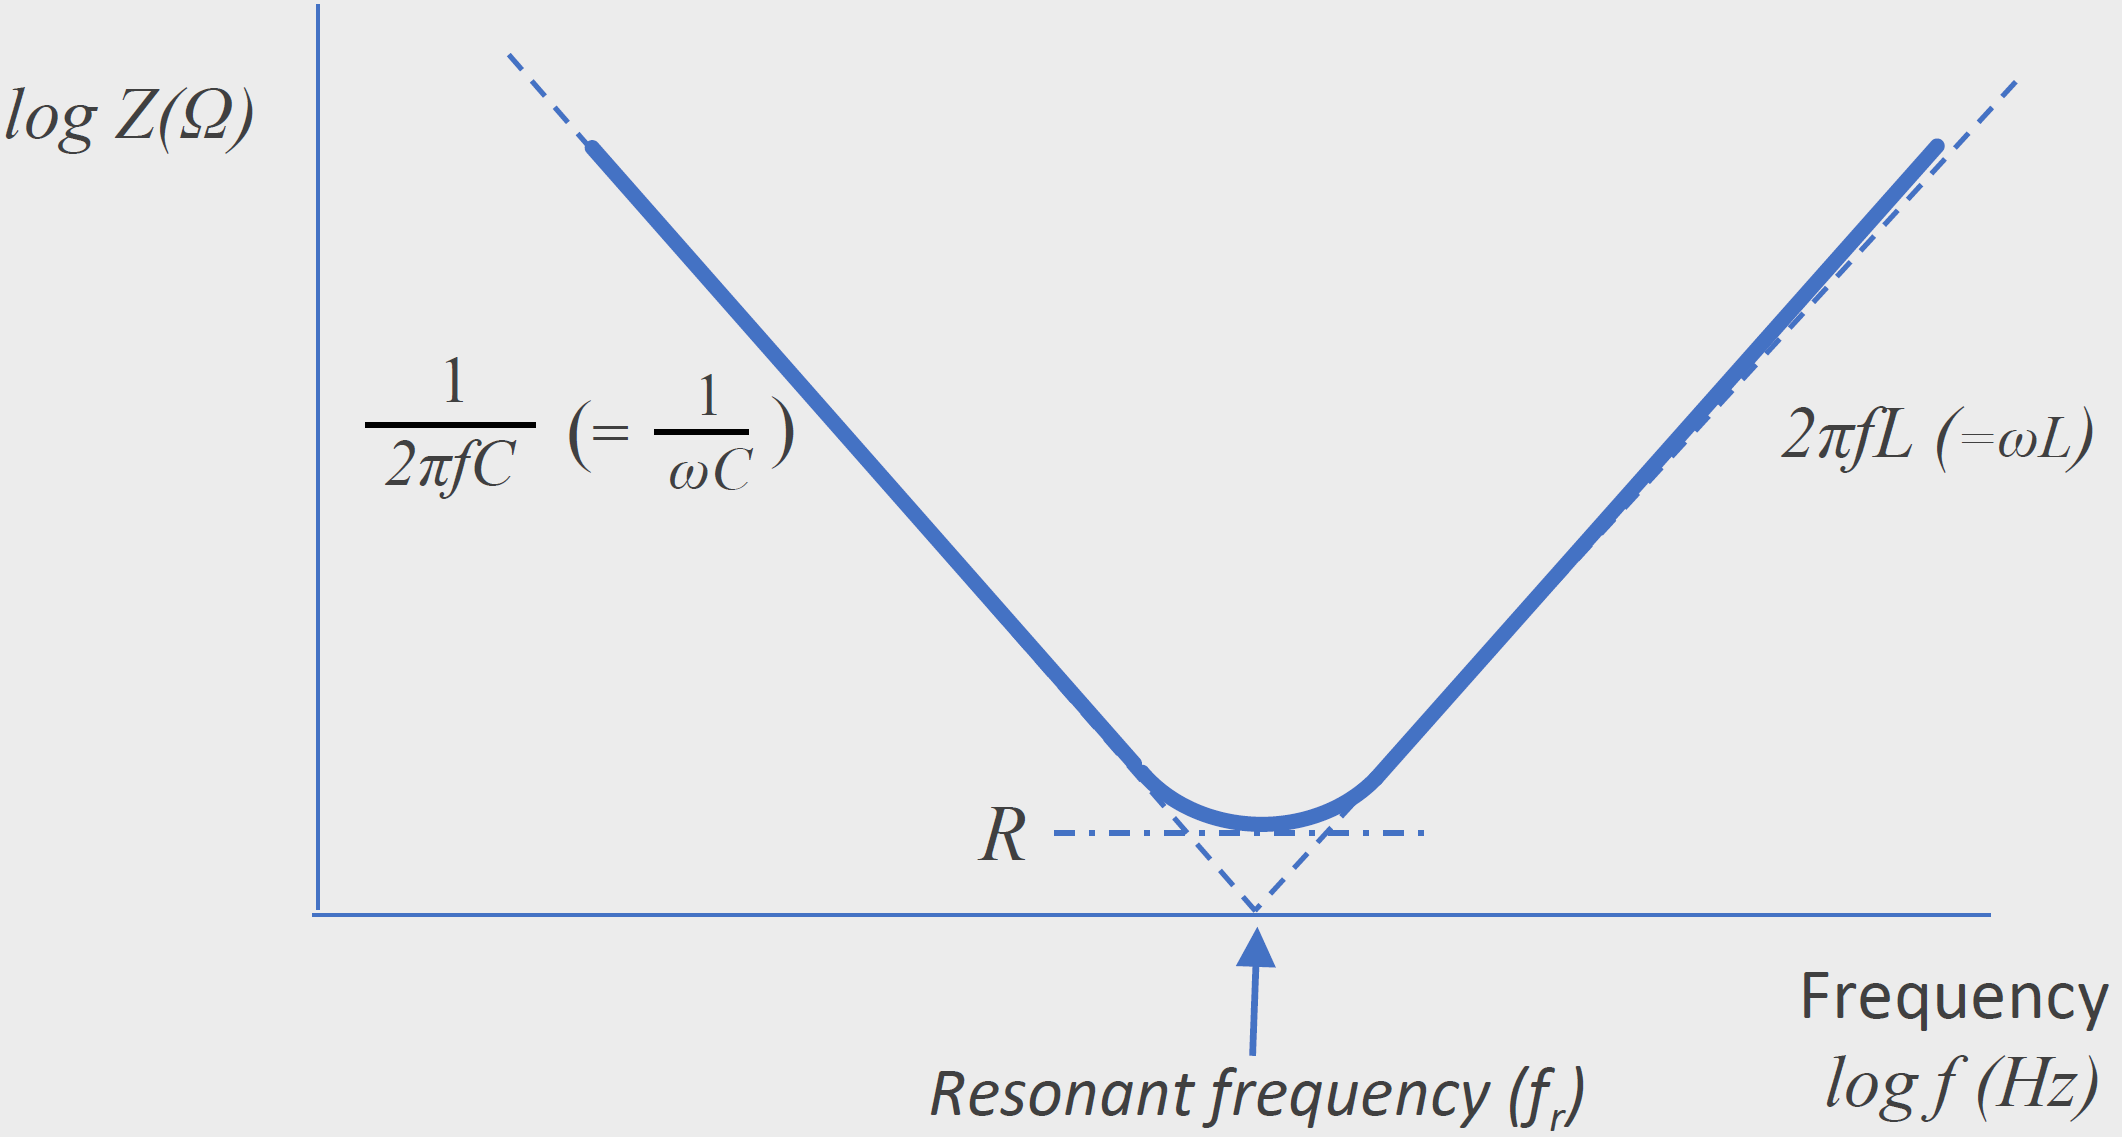
\includegraphics[width=\linewidth]{fig/lec08/impedance_vs_frequency.png}
    \caption{Schematic impedance curve of a real capacitor showing capacitive, resistive, and inductive regions. Adapted from AIC tech, \textit{The Three Essential Characteristics of Capacitors}}
\end{figure}
\end{column}
\end{columns}

\end{frame}


%%%%%%%%%%%%%%%%%%%%%%%%%%%%%%%%%%%%%%%%%%%%%%%%%%%%%%%%%%%%%
%% Self resonant frequency
%%%%%%%%%%%%%%%%%%%%%%%%%%%%%%%%%%%%%%%%%%%%%%%%%%%%%%%%%%%%%
\begin{frame}
\frametitle{Self-Resonant Frequency}
\begin{columns}
\begin{column}{0.56\textwidth}
The self-resonant frequency occurs when the capacitive and inductive reactances cancel:
\begin{align}
    \omega_0 L_{\mathrm{ESL}}
    =
    \frac{1}{\omega_0 C}
\end{align}
\begin{align}
    f_{\mathrm{SRF}}
    =
    \frac{1}{2\pi\sqrt{L_{\mathrm{ESL}}C}}
\end{align}
Below $f_{\mathrm{SRF}}$:
\begin{align}
    |X_C| > |X_L|
\end{align}
and the component behaves mainly as a capacitor. Above $f_{\mathrm{SRF}}$:
\begin{align}
    |X_L| > |X_C|
\end{align}
and the component behaves mainly as an inductor.
\end{column}

\begin{column}{0.40\textwidth}
\begin{block}{Practical Rule}
Do not assume that a large capacitor is useful at all frequencies. Large electrolytics are effective at low frequencies, while small ceramics are effective at much higher frequencies.
\end{block}
\begin{block}{Design Implication}
For high-frequency decoupling, low ESL and short mounting paths are often more important than large capacitance.
\end{block}
\end{column}
\end{columns}
\end{frame}


%%%%%%%%%%%%%%%%%%%%%%%%%%%%%%%%%%%%%%%%%%%%%%%%%%%%%%%%%%%%%
%% Impedance of different capacitor technologies
%%%%%%%%%%%%%%%%%%%%%%%%%%%%%%%%%%%%%%%%%%%%%%%%%%%%%%%%%%%%%
\begin{frame}
\frametitle{Impedance of Different Capacitor Technologies}
\begin{columns}
\begin{column}{0.56\textwidth}
Different capacitor technologies are effective over different frequency ranges.
\begin{itemize}
    \item \textbf{Aluminum electrolytic capacitors}
    \begin{itemize}
        \item high capacitance,
        \item useful for low-frequency energy buffering,
        \item higher ESR and ESL.
    \end{itemize}

    \item \textbf{Film capacitors}
    \begin{itemize}
        \item lower loss,
        \item high ripple-current capability,
        \item useful for DC-link and snubber applications.
    \end{itemize}

    \item \textbf{MLCCs}
    \begin{itemize}
        \item very low ESL,
        \item effective at high frequency,
        \item capacitance may strongly depend on DC bias.
    \end{itemize}
\end{itemize}
A practical converter often uses a capacitor bank combining several technologies.
\end{column}

\begin{column}{0.40\textwidth}
\begin{figure}
    \centering
    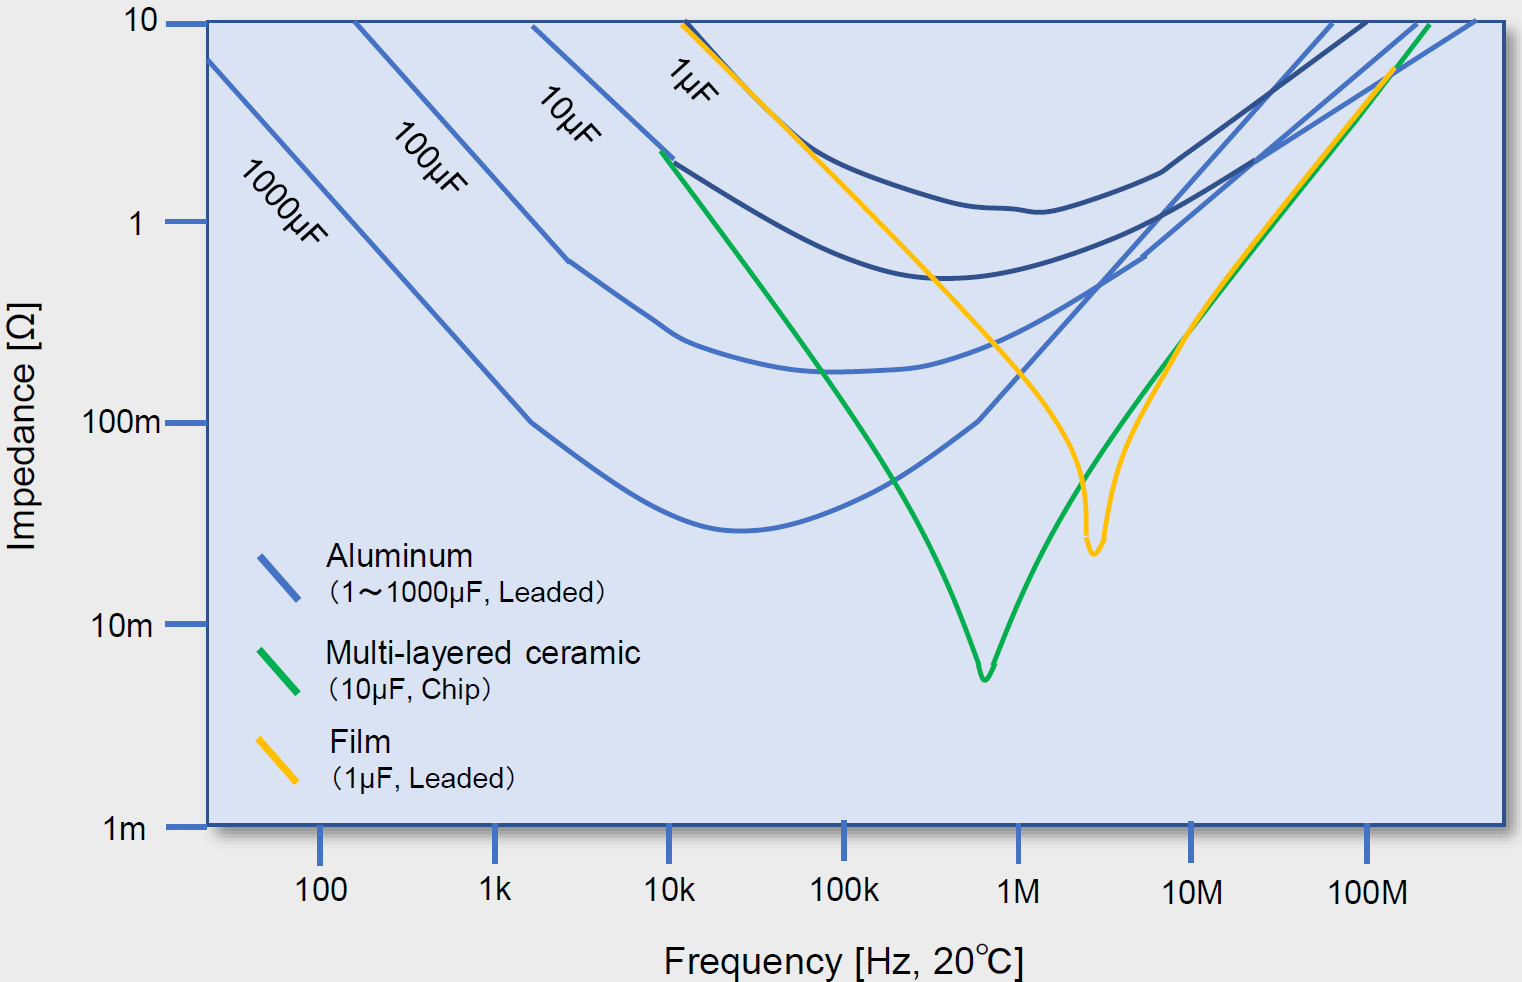
\includegraphics[width=\linewidth]{fig/lec08/impedance_various_capacitors.png}
    \caption{Impedance versus frequency for aluminum electrolytic, film, and multilayer ceramic capacitors. Adapted from AIC tech, \textit{The Three Essential Characteristics of Capacitors}}
\end{figure}
\end{column}
\end{columns}

\end{frame}


%%%%%%%%%%%%%%%%%%%%%%%%%%%%%%%%%%%%%%%%%%%%%%%%%%%%%%%%%%%%%
%% Parallel capacitor networks
%%%%%%%%%%%%%%%%%%%%%%%%%%%%%%%%%%%%%%%%%%%%%%%%%%%%%%%%%%%%%
\begin{frame}
\frametitle{Why are Multiple Capacitors Connected in Parallel?}
\begin{columns}
\begin{column}{0.55\textwidth}
A single capacitor type cannot provide low impedance over a wide frequency range. Therefore, practical converters often combine:
\begin{itemize}
    \item \textbf{bulk capacitor:} low-frequency energy storage,
    \item \textbf{film or polymer capacitor:} mid-frequency ripple current,
    \item \textbf{ceramic capacitor:} high-frequency switching current,
    \item \textbf{local decoupling capacitor:} device-level transient current.
\end{itemize}
For capacitors in parallel,
\begin{align}
    C_{\mathrm{eq}} = C_1+C_2+C_3+\cdots
\end{align}
\end{column}

\begin{column}{0.41\textwidth}
\begin{center}
\begin{circuitikz}[scale=0.78, transform shape]
    \draw (0,0) -- (4.0,0);
    \draw (0,-2.5) -- (4.0,-2.5);

    \draw (0.6,0) to[C,l=$C_{\mathrm{bulk}}$] (0.6,-2.5);
    \draw (1.8,0) to[C,l=$C_{\mathrm{film}}$] (1.8,-2.5);
    \draw (3.0,0) to[C,l=$C_{\mathrm{cer}}$] (3.0,-2.5);

    \draw[->, thick] (-0.5,-1.25) -- (0.2,-1.25);
    \node at (-0.85,-1.25) {$i_C$};

    \node at (0.6,-3.0) {\scriptsize low $f$};
    \node at (1.8,-3.0) {\scriptsize mid $f$};
    \node at (3.0,-3.0) {\scriptsize high $f$};
\end{circuitikz}
\end{center}

\begin{block}{Layout Warning}
The high-frequency capacitor must be physically close to the switching loop. Otherwise PCB and busbar inductance dominate the impedance.
\end{block}
\end{column}
\end{columns}
and ideally ESR and ESL reduce. In practice, layout determines whether this benefit is achieved.
\end{frame}


%%%%%%%%%%%%%%%%%%%%%%%%%%%%%%%%%%%%%%%%%%%%%%%%%%%%%%%%%%%%%
%% Capacitor impedance network
%%%%%%%%%%%%%%%%%%%%%%%%%%%%%%%%%%%%%%%%%%%%%%%%%%%%%%%%%%%%%
\begin{frame}
\frametitle{Impedance Target of a Capacitor Network}
\begin{columns}
\begin{column}{0.56\textwidth}
In a regulator or converter, the objective is usually not to minimize the impedance of one capacitor, but to shape the total impedance of the full capacitor network. Important design ideas:
\begin{itemize}
    \item The bulk capacitor controls low-frequency energy demand.
    \item Polymer or film capacitors reduce mid-frequency impedance.
    \item MLCCs reduce high-frequency impedance.
    \item Excessively low impedance at some frequencies can interact with the control loop and reduce damping.
    \item The impedance at the actual load terminals can differ from the impedance at the regulator terminals due to PCB parasitics.
\end{itemize}
Therefore, capacitor selection should be performed together with layout and stability analysis.
\end{column}

\begin{column}{0.40\textwidth}
\begin{figure}
    \centering
    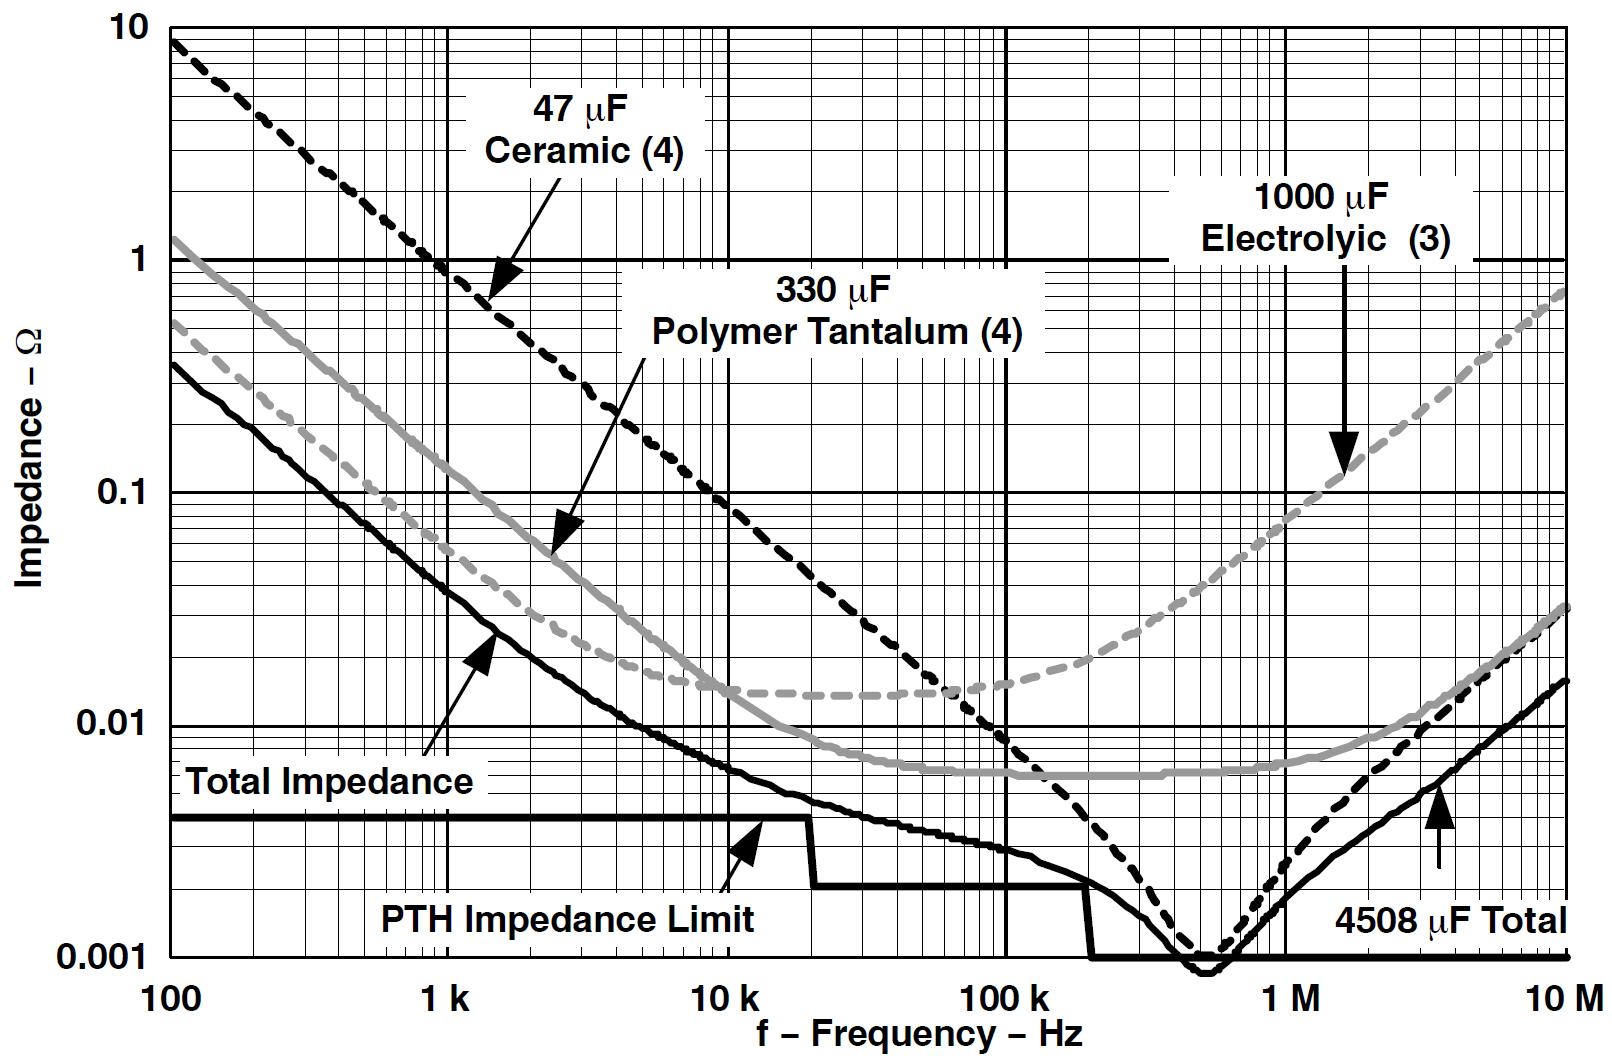
\includegraphics[width=\linewidth]{fig/lec08/impedance_limits.png}
    \caption{Output capacitor impedance limits and combined impedance of electrolytic, polymer tantalum, and ceramic capacitor networks. Adapted from Texas Instruments, \textit{Input and Output Capacitor Selection}}
\end{figure}
\end{column}
\end{columns}
\end{frame}


%%%%%%%%%%%%%%%%%%%%%%%%%%%%%%%%%%%%%%%%%%%%%%%%%%%%%%%%%%%%%
%% Leakage current
%%%%%%%%%%%%%%%%%%%%%%%%%%%%%%%%%%%%%%%%%%%%%%%%%%%%%%%%%%%%%
\begin{frame}
\frametitle{Leakage Current and Insulation Resistance}

\begin{columns}
\begin{column}{0.5\textwidth}
A real capacitor does not perfectly block DC. A small leakage current flows through or around the dielectric. Leakage current can be represented by an insulation resistance in parallel with the capacitance:
\begin{align}
    i_{\mathrm{leak}}
    =
    \frac{V}{R_{\mathrm{iso}}}
\end{align}
where,
\begin{itemize}
    \item $i_{\mathrm{leak}}$ is leakage current,
    \item $V$ is applied voltage,
    \item $R_{\mathrm{iso}}$ is insulation resistance.
\end{itemize}

\end{column}

\begin{column}{0.5\textwidth}
    Leakage current is important for:
\begin{itemize}
    \item DC-link discharge behaviour,
    \item capacitor bank voltage balancing,
    \item standby power loss,
    \item safety after shutdown,
    \item health monitoring and ageing assessment.
\end{itemize}
\begin{figure}
    \centering
    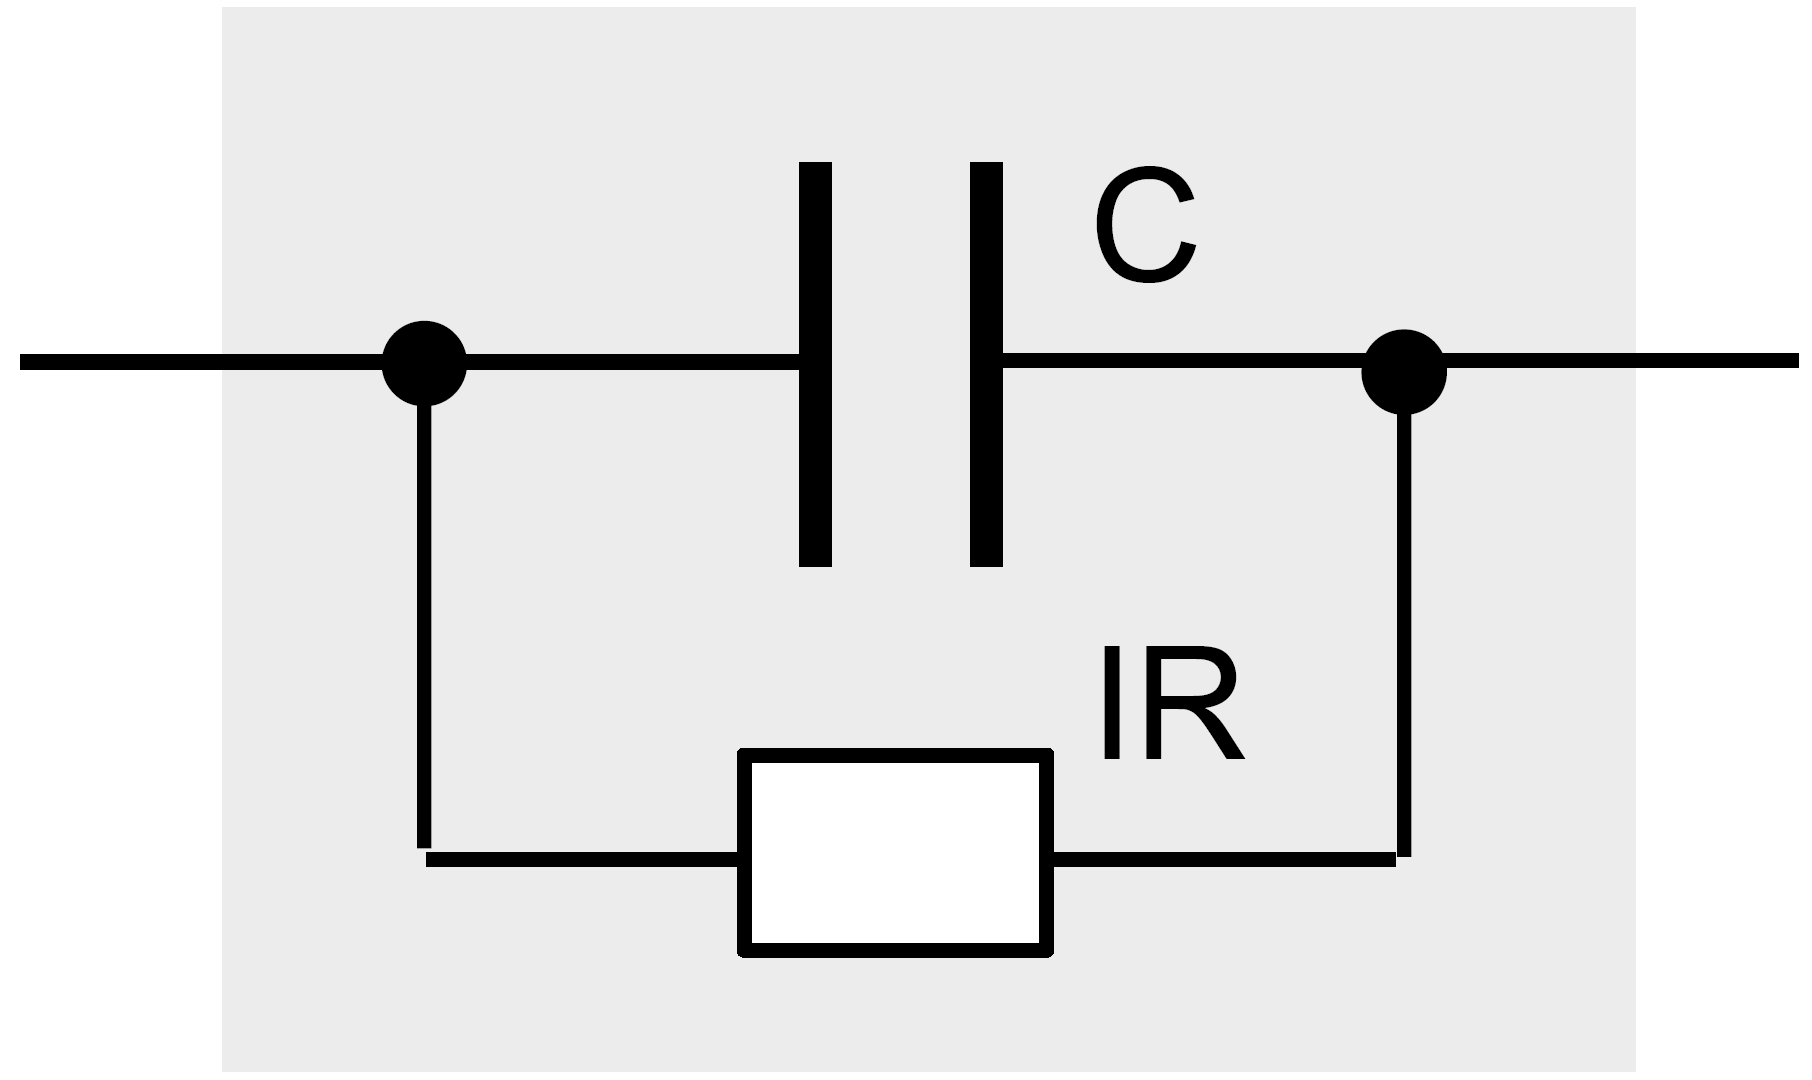
\includegraphics[width=0.3\linewidth]{fig/lec08/capacitance_insulation_resistance.png}
    \caption{Leakage current represented by insulation resistance in parallel with capacitance. Adapted from AIC tech, \textit{The Three Essential Characteristics of Capacitors}}
\end{figure}
\end{column}
\end{columns}

\end{frame}


%%%%%%%%%%%%%%%%%%%%%%%%%%%%%%%%%%%%%%%%%%%%%%%%%%%%%%%%%%%%%
%% Leakage current dependence
%%%%%%%%%%%%%%%%%%%%%%%%%%%%%%%%%%%%%%%%%%%%%%%%%%%%%%%%%%%%%
\begin{frame}
\frametitle{Leakage Current Depends on Voltage, Temperature, and History}
\begin{columns}
\begin{column}{0.56\textwidth}
Leakage current is not a fixed constant. It depends strongly on operating condition and capacitor technology. Important dependencies:
\begin{itemize}
    \item Leakage current increases with applied voltage.
    \item Leakage current usually increases with temperature.
    \item Electrolytic capacitor leakage depends on formation condition and voltage history.
    \item Humidity, contamination, dielectric defects, and ageing can increase leakage.
\end{itemize}
For capacitor banks, leakage mismatch is especially important because it can cause unequal voltage sharing between series-connected capacitors. Therefore, series capacitor banks usually require voltage-balancing resistors.
\end{column}

\begin{column}{0.40\textwidth}
\begin{figure}
    \centering
    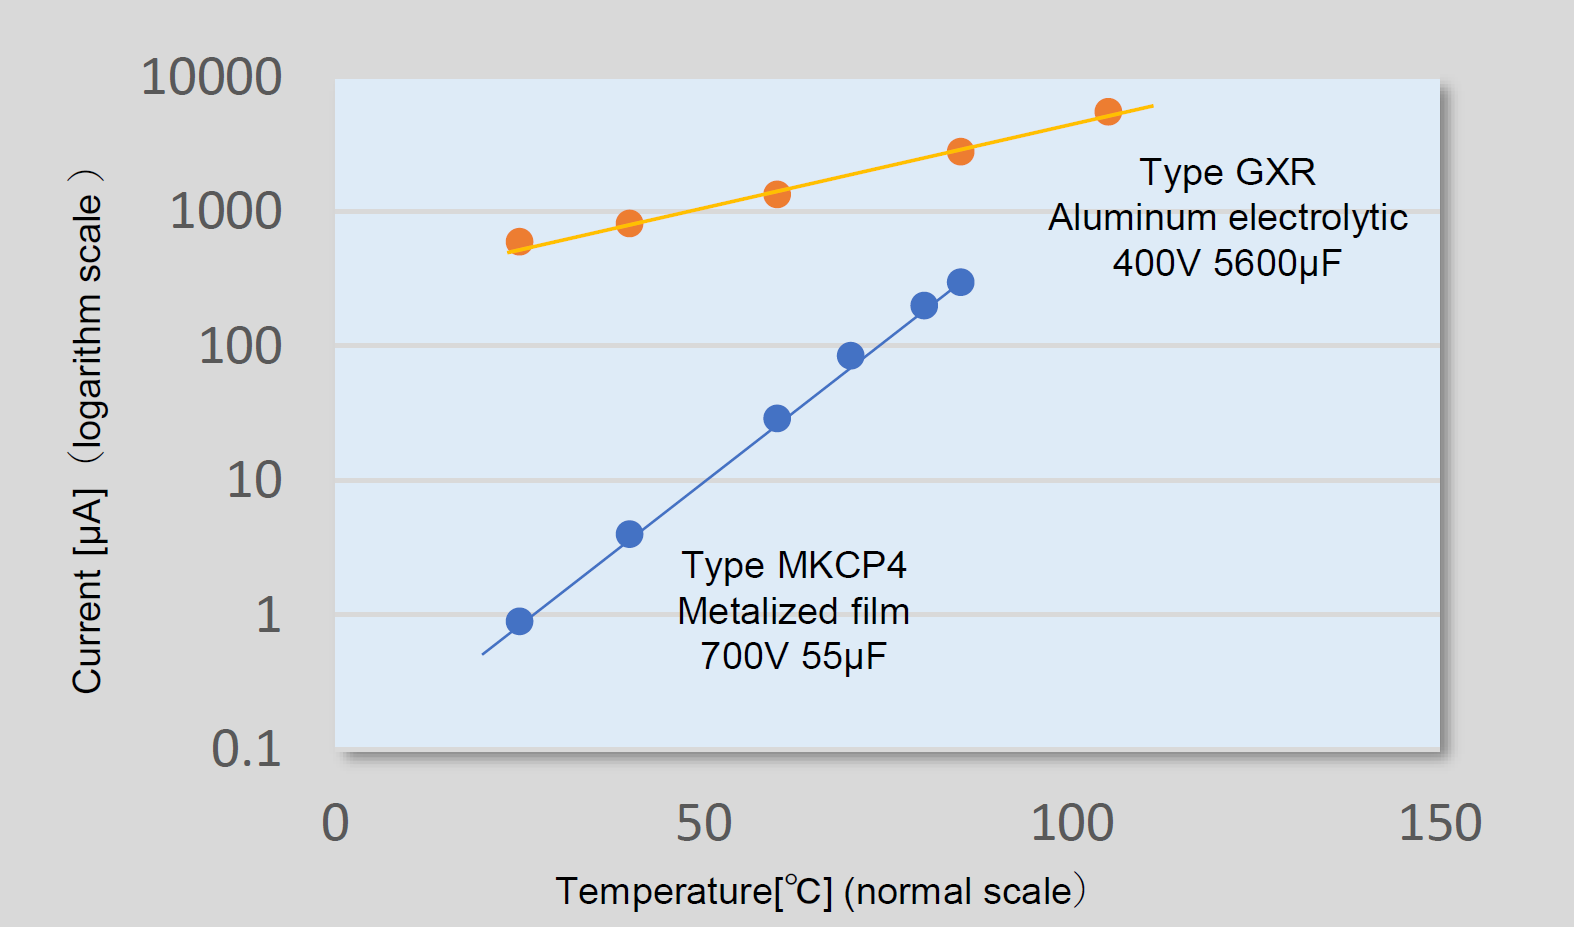
\includegraphics[width=\linewidth]{fig/lec08/leakage_temperature.png}
    \caption{Leakage current versus temperature for aluminum electrolytic and metallized film capacitors. Adapted from AIC tech, \textit{The Three Essential Characteristics of Capacitors}}
\end{figure}
\end{column}
\end{columns}

\end{frame}


%%%%%%%%%%%%%%%%%%%%%%%%%%%%%%%%%%%%%%%%%%%%%%%%%%%%%%%%%%%%%
%% Dissipation factor and tan delta
%%%%%%%%%%%%%%%%%%%%%%%%%%%%%%%%%%%%%%%%%%%%%%%%%%%%%%%%%%%%%
\begin{frame}
\frametitle{Dissipation Factor and $\tan\delta$}
\begin{columns}
\begin{column}{0.56\textwidth}
In an ideal capacitor, the current leads the voltage by exactly $90^\circ$. In a real capacitor, losses reduce this phase angle slightly. The dissipation factor is commonly written as
\begin{align}
    \tan\delta
    =
    \frac{R_{\mathrm{ESR}}}{X_C}
    =
    \omega C R_{\mathrm{ESR}}
\end{align}
where
\begin{align}
    X_C=\frac{1}{\omega C}
\end{align}
A smaller $\tan\delta$ means lower dielectric and resistive loss. For sinusoidal operation, dielectric loss can be estimated using
\begin{align}
    P_{\mathrm{diel}}
    =
    \omega C V_{\mathrm{rms}}^2 \tan\delta
\end{align}
\end{column}

\begin{column}{0.40\textwidth}
\begin{figure}
    \centering
    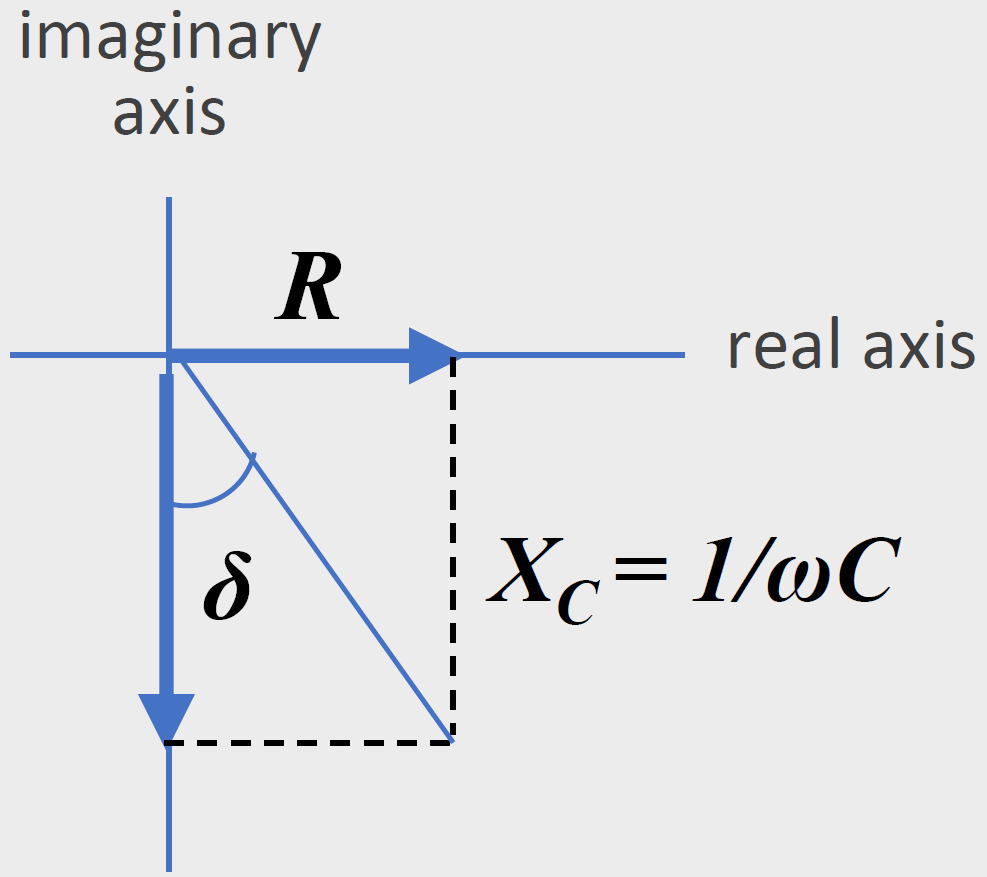
\includegraphics[width=0.5\linewidth]{fig/lec08/vector_R_Xc_tandelta.png}
    \caption{Vector expression of resistance and capacitive reactance used to define $\tan\delta$. Adapted from AIC tech, \textit{The Three Essential Characteristics of Capacitors}}
\end{figure}
\end{column}
\end{columns}

\end{frame}


%%%%%%%%%%%%%%%%%%%%%%%%%%%%%%%%%%%%%%%%%%%%%%%%%%%%%%%%%%%%%
%% Equivalent circuit for sinusoidal loss
%%%%%%%%%%%%%%%%%%%%%%%%%%%%%%%%%%%%%%%%%%%%%%%%%%%%%%%%%%%%%
\begin{frame}
\frametitle{Equivalent Circuits for Capacitor Losses}
\begin{columns}
\begin{column}{0.56\textwidth}
Capacitor losses are often represented using either a parallel or series equivalent circuit. For sinusoidal operation, the two forms can be transformed into one another. The series representation is especially useful in power electronics because ripple current directly produces ESR loss:
\begin{align}
    P_{\mathrm{loss}}
    =
    I_{\mathrm{rms}}^2R_{\mathrm{ESR}}
\end{align}
The parallel representation is useful for interpreting insulation resistance and dielectric leakage. For non-sinusoidal power-converter waveforms, losses should be evaluated from the harmonic content or measured under realistic operating conditions.
\end{column}

\begin{column}{0.40\textwidth}
\begin{figure}
    \centering
    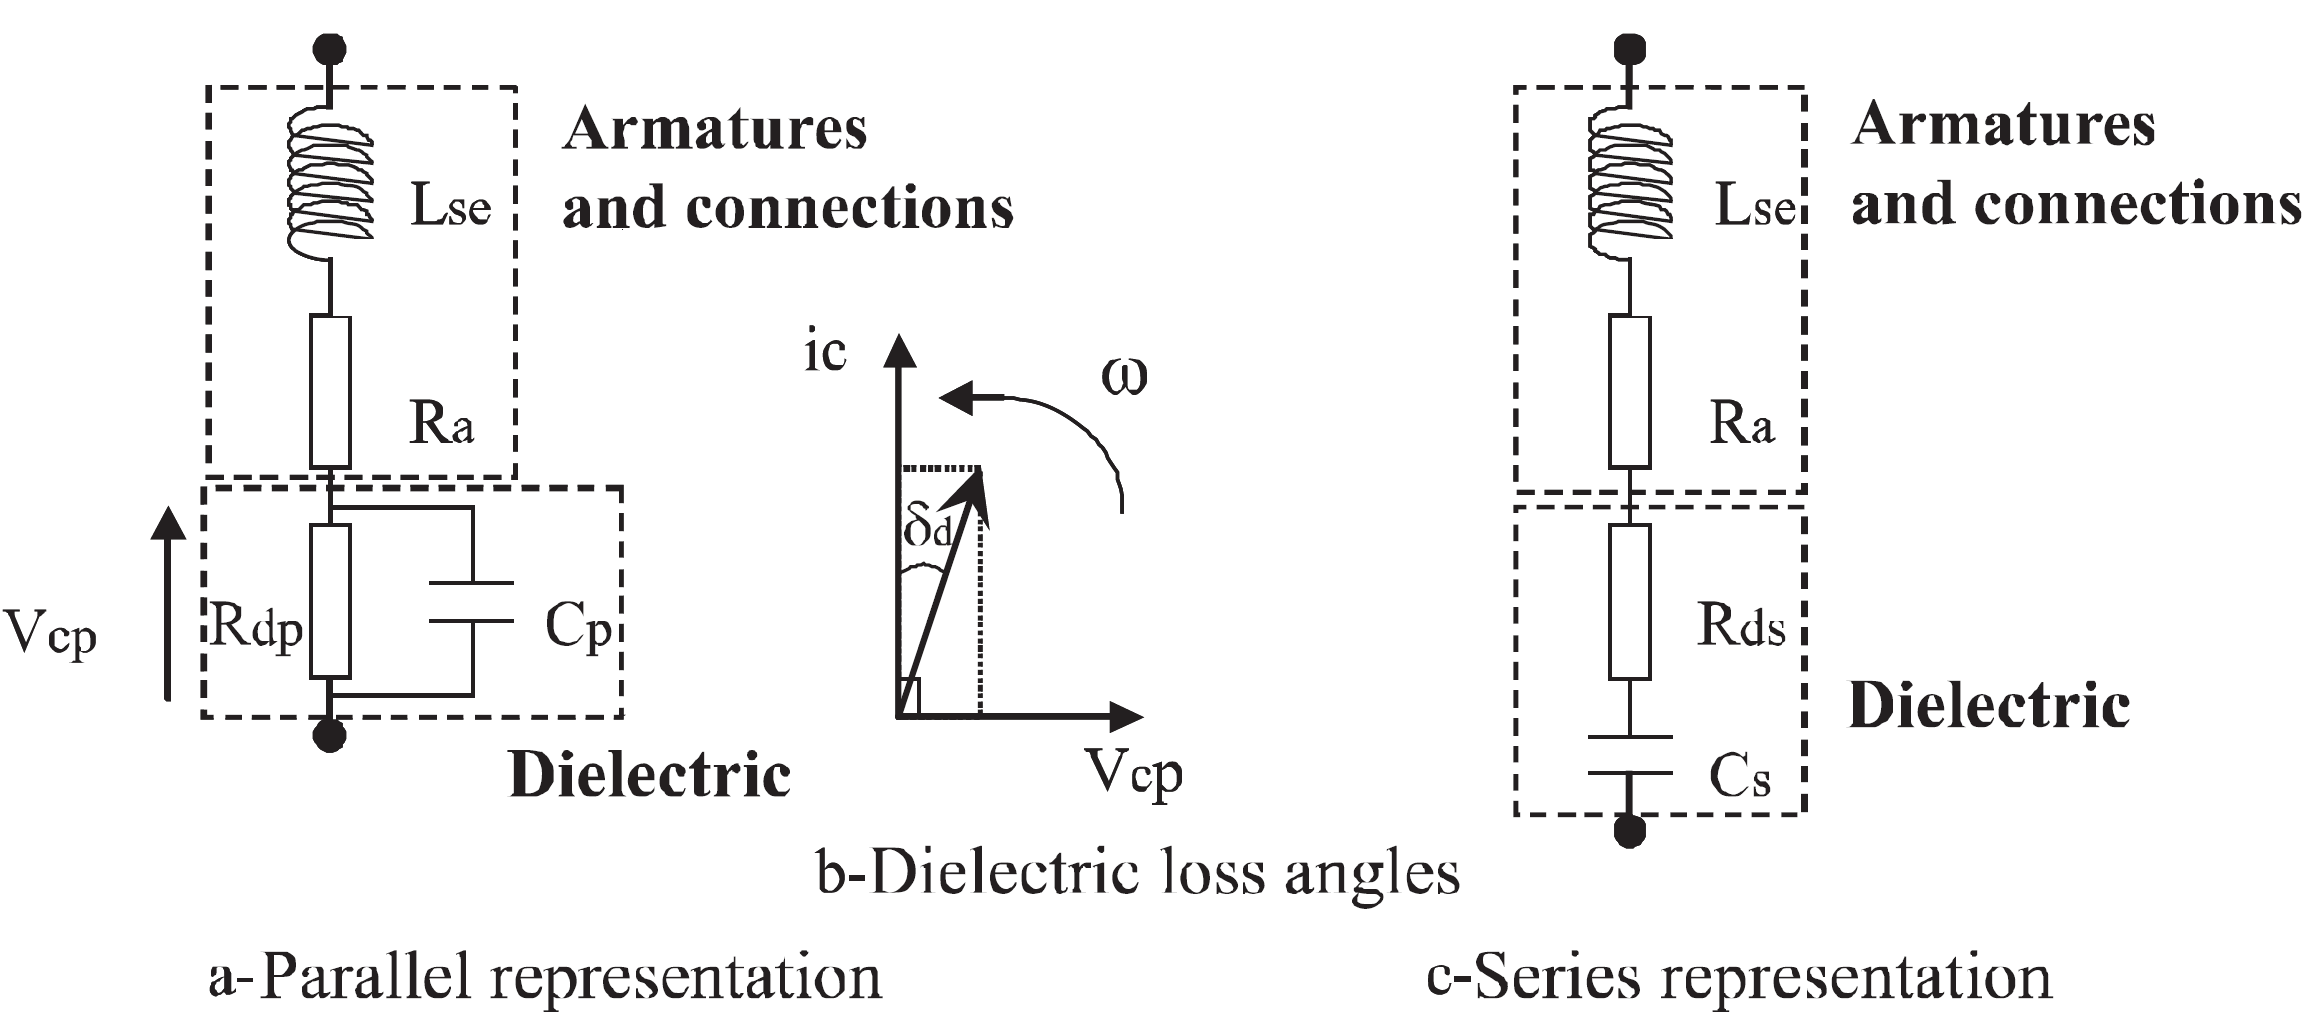
\includegraphics[width=\linewidth]{fig/lec08/capacitor_equivalent_circuits.png}
    \caption{Parallel and series equivalent electrical circuits of a capacitor under sinusoidal operation. Adapted from Perret, \textit{Power Electronics Semiconductor Devices}, Wiley, 2009.}
\end{figure}
\end{column}
\end{columns}
\end{frame}


%%%%%%%%%%%%%%%%%%%%%%%%%%%%%%%%%%%%%%%%%%%%%%%%%%%%%%%%%%%%%
%% Dielectric absorption
%%%%%%%%%%%%%%%%%%%%%%%%%%%%%%%%%%%%%%%%%%%%%%%%%%%%%%%%%%%%%
\begin{frame}
\frametitle{Dielectric Absorption and Recovery Voltage}

\begin{columns}
\begin{column}{0.56\textwidth}
Dielectric absorption is when a capacitor regains a small voltage after being discharged and left open-circuited:
\begin{itemize}
    \item Polarization processes inside the dielectric are not instantaneous.
    \item Some dipoles relax slowly after the external voltage is removed.
    \item Charge redistribution can produce a residual recovery voltage.
\end{itemize}
\end{column}

\begin{column}{0.40\textwidth}
\begin{figure}
    \centering
    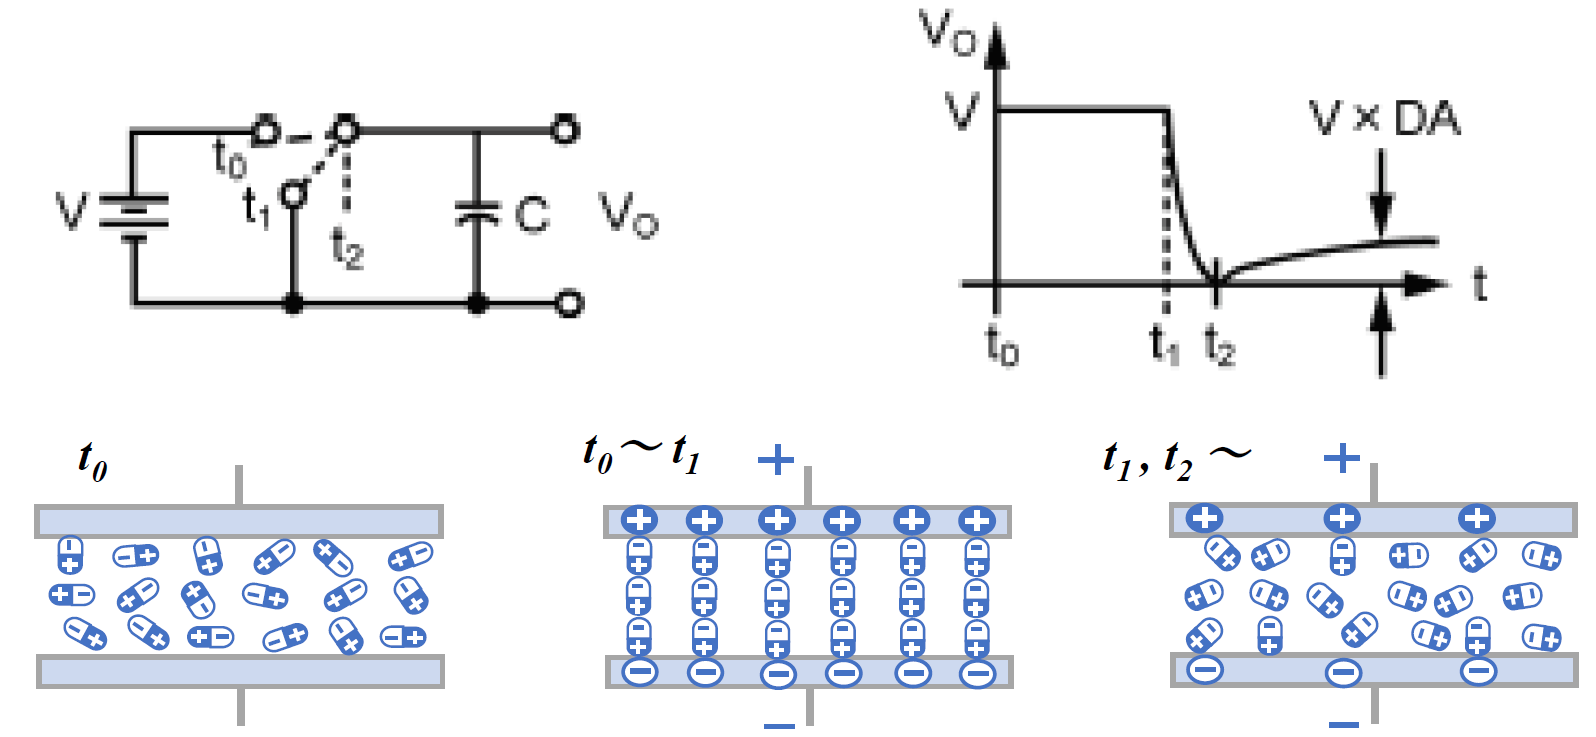
\includegraphics[width=\linewidth]{fig/lec08/dielectric_absorption_and_recovery_voltage.png}
    \caption{Dielectric absorption and recovery voltage after short-circuit discharge. Adapted from AIC tech, \textit{The Three Essential Characteristics of Capacitors}}
\end{figure}
\end{column}
\end{columns}

\end{frame}



%%%%%%%%%%%%%%%%%%%%%%%%%%%%%%%%%%%%%%%%%%%%%%%%%%%%%%%%%%%%%
%% Dielectric absorption
%%%%%%%%%%%%%%%%%%%%%%%%%%%%%%%%%%%%%%%%%%%%%%%%%%%%%%%%%%%%%
\begin{frame}
\frametitle{Dielectric Absorption and Recovery Voltage}
\begin{columns}
\begin{column}{0.56\textwidth}
Dielectric absorption effect is important in:
\begin{itemize}
    \item precision sampling circuits,
    \item high-voltage DC-link safety,
    \item insulation testing,
    \item pulse capacitors,
    \item stored-energy applications.
\end{itemize}
A discharged capacitor should therefore still be treated carefully in high-voltage systems.
\end{column}

\begin{column}{0.40\textwidth}
\begin{block}{Practical Safety Message}
\small
Large capacitors may show recovery voltage after discharge due to dielectric absorption. Discharge resistors and voltage verification are required before handling high-energy capacitor banks.
\end{block}
\end{column}
\end{columns}
\end{frame}


%%%%%%%%%%%%%%%%%%%%%%%%%%%%%%%%%%%%%%%%%%%%%%%%%%%%%%%%%%%%%
%% Real capacitor design summary
%%%%%%%%%%%%%%%%%%%%%%%%%%%%%%%%%%%%%%%%%%%%%%%%%%%%%%%%%%%%%
\begin{frame}
\frametitle{Summary: What Defines a Real Capacitor?}
\begin{itemize}
    \item Capacitance determines ideal charge storage: $Q=CV$.
    \item ESR determines ripple-current heating: $P_{\mathrm{ESR}}=I_{\mathrm{rms}}^2R_{\mathrm{ESR}}$.
    \item ESL determines high-frequency voltage spikes:
    \begin{align}
        v_{\mathrm{ESL}}=L_{\mathrm{ESL}}\frac{di}{dt}
    \end{align}
    \item Self-resonant frequency separates capacitive and inductive behaviour:
    \begin{align}
        f_{\mathrm{SRF}}=\frac{1}{2\pi\sqrt{L_{\mathrm{ESL}}C}}
    \end{align}
    \item Leakage current affects safety, voltage balancing, standby loss, and ageing:
    \begin{align}
        i_{\mathrm{leak}}=\frac{V}{R_{\mathrm{iso}}}
    \end{align}
    \item In power electronics, the useful capacitor is the one that gives the required impedance, ripple-current capability, thermal margin, and lifetime in the actual converter layout.
\end{itemize}

\end{frame}

%%%%%%%%%%%%%%%%%%%%%%%%%%%%%%%%%%%%%%%%%%%%%%%%%%%%%%%%%%%%%
%% Capacitors in converter applications
%%%%%%%%%%%%%%%%%%%%%%%%%%%%%%%%%%%%%%%%%%%%%%%%%%%%%%%%%%%%%
\begin{frame}
\begin{center}
  \textbf{\Huge{Capacitors in Converter Applications}}\\[0.4cm]
  \textbf{\Large{Input, Output, DC-Link, Snubber, Resonant, and Filter Capacitors}}
\end{center}
\end{frame}


%%%%%%%%%%%%%%%%%%%%%%%%%%%%%%%%%%%%%%%%%%%%%%%%%%%%%%%%%%%%%
%% Capacitor placement in power converters
%%%%%%%%%%%%%%%%%%%%%%%%%%%%%%%%%%%%%%%%%%%%%%%%%%%%%%%%%%%%%
\begin{frame}
\frametitle{Where are Capacitors Used in a Power Converter?}

\begin{columns}
\begin{column}{0.58\textwidth}
Capacitors appear at several locations in a power electronic system. Each location imposes different stress and requires a distinct design approach.
\begin{itemize}
    \item \textbf{Input filter capacitor:} reduces source-side ripple and reflected switching noise.
    \item \textbf{DC-link capacitor:} buffers energy and stabilizes the intermediate DC voltage.
    \item \textbf{Local decoupling capacitor:} supplies very fast switching current close to semiconductor devices.
    \item \textbf{Snubber capacitor:} limits overvoltage during switching transients.
    \item \textbf{Output capacitor:} reduces output-voltage ripple and supports load transients.
    \item \textbf{AC harmonic filter capacitor:} attenuates switching-frequency harmonics at the AC side.
\end{itemize}
Thus, capacitor selection must always begin with the converter function.
\end{column}

\begin{column}{0.38\textwidth}
\begin{figure}
    \centering
    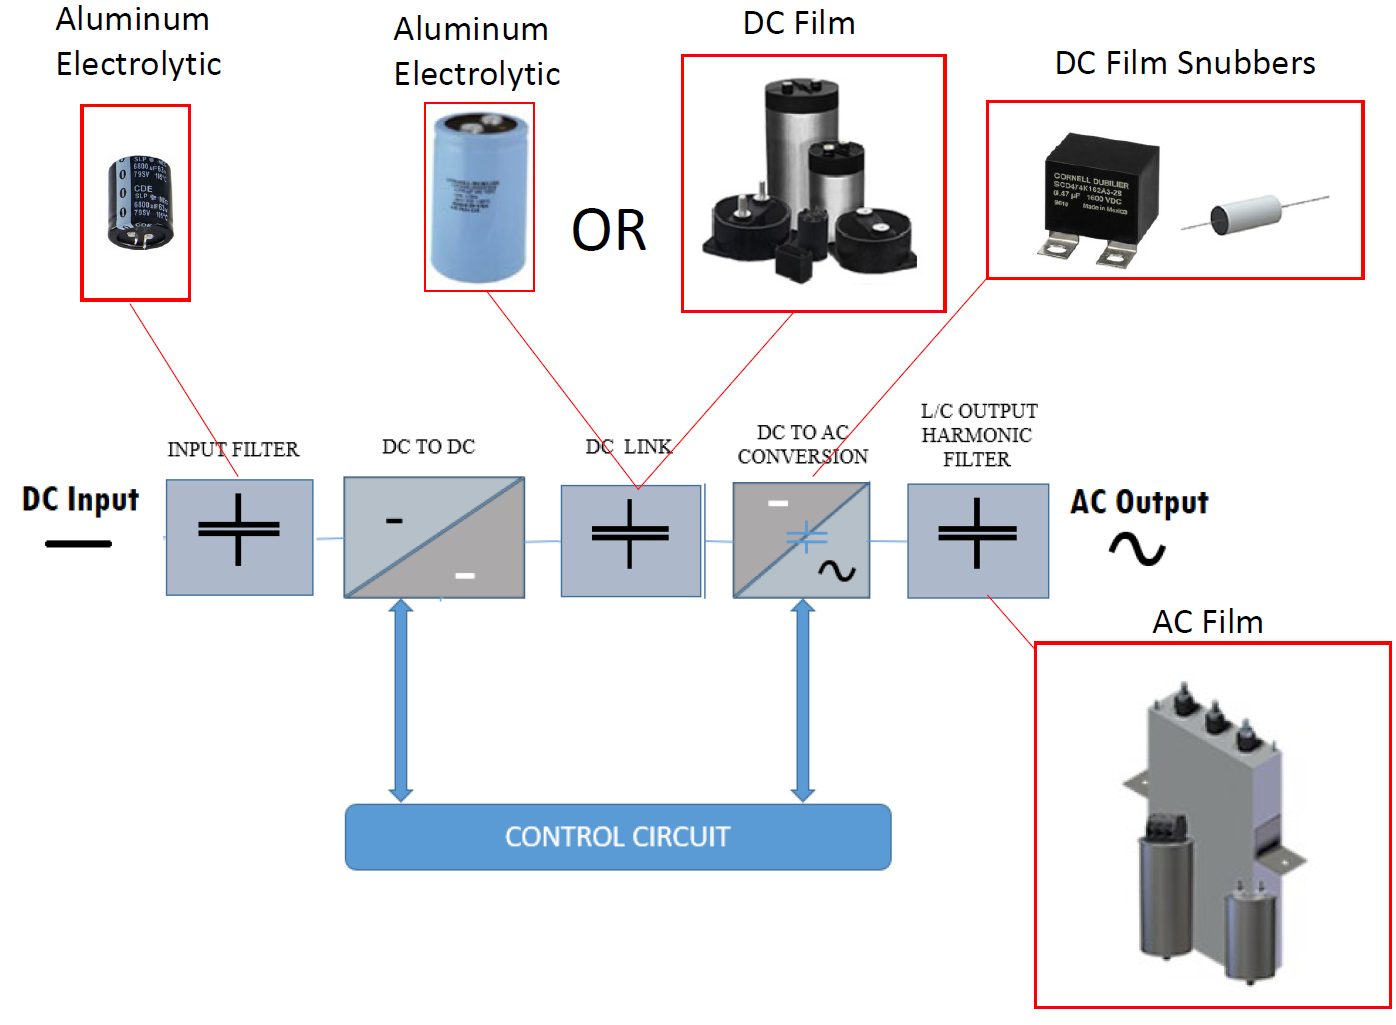
\includegraphics[width=\linewidth]{fig/lec08/capacitors_types.png}
    \caption{Capacitor locations in inverter and converter systems: input filter, DC-link, snubber, and AC harmonic filter. Adapted from Cornell Dubilier, \textit{Capacitors for High Power Inverters and Converters}}
\end{figure}
\end{column}
\end{columns}

\end{frame}


%%%%%%%%%%%%%%%%%%%%%%%%%%%%%%%%%%%%%%%%%%%%%%%%%%%%%%%%%%%%%
%% Application map using circuitikz
%%%%%%%%%%%%%%%%%%%%%%%%%%%%%%%%%%%%%%%%%%%%%%%%%%%%%%%%%%%%%
\begin{frame}
\frametitle{Capacitor Function Map in a Converter}
\begin{center}
\begin{circuitikz}[scale=0.77, transform shape]
    \tikzstyle{block} = [draw, rounded corners, align=center,
    minimum width=2.35cm, minimum height=0.78cm, font=\scriptsize]

    \node[block] (source) at (0,0) {DC or AC\\source};
    \node[block] (input) at (2.8,0) {Input\\filter};
    \node[block] (stage1) at (5.6,0) {Rectifier /\\DC--DC};
    \node[block] (dclink) at (8.4,0) {DC link};
    \node[block] (stage2) at (11.2,0) {Inverter /\\DC--DC};
    \node[block] (output) at (14.0,0) {Output\\filter};
    \node[block] (load) at (16.6,0) {Load};

    \draw[->, thick] (source) -- (input);
    \draw[->, thick] (input) -- (stage1);
    \draw[->, thick] (stage1) -- (dclink);
    \draw[->, thick] (dclink) -- (stage2);
    \draw[->, thick] (stage2) -- (output);
    \draw[->, thick] (output) -- (load);

    \node at (2.8,-1.05) {\scriptsize $C_{\mathrm{in}}$};
    \node at (8.4,-1.05) {\scriptsize $C_{\mathrm{dc}}$};
    \node at (11.2,-1.05) {\scriptsize $C_{\mathrm{snub}}$};
    \node at (14.0,-1.05) {\scriptsize $C_{\mathrm{out}}$};

    \draw (2.8,-0.55) to[C] (2.8,-1.55);
    \draw (8.4,-0.55) to[C] (8.4,-1.55);
    \draw (11.2,-0.55) to[C] (11.2,-1.55);
    \draw (14.0,-0.55) to[C] (14.0,-1.55);

    \node[align=center, font=\scriptsize] at (2.8,-2.05) {ripple and\\EMI reduction};
    \node[align=center, font=\scriptsize] at (8.4,-2.05) {energy buffer and\\DC-bus stabilization};
    \node[align=center, font=\scriptsize] at (11.2,-2.05) {switching\\overvoltage control};
    \node[align=center, font=\scriptsize] at (14.0,-2.05) {output ripple and\\transient support};
\end{circuitikz}
\end{center}

\begin{block}{Teaching Message}
The same symbol \(C\) can represent very different hardware requirements depending on its converter location. A DC-link capacitor, snubber capacitor, and output capacitor are not interchangeable design objects.
\end{block}

\end{frame}


%%%%%%%%%%%%%%%%%%%%%%%%%%%%%%%%%%%%%%%%%%%%%%%%%%%%%%%%%%%%%
%% Input capacitor in buck converter
%%%%%%%%%%%%%%%%%%%%%%%%%%%%%%%%%%%%%%%%%%%%%%%%%%%%%%%%%%%%%
\begin{frame}
\frametitle{Input Capacitor in a Buck Converter}

\begin{columns}
\begin{column}{0.56\textwidth}
The buck input capacitor supplies the switch-node pulsed current and limits input-source ripple voltage. For a single-phase buck converter:
\begin{itemize}
    \item the input capacitor current is strongly pulsed,
    \item the RMS ripple current depends on duty cycle,
    \item worst ripple-current stress near \(D=0.5\),
    \item ceramic capacitors are required close to the switching stage for high-frequency ripple control,
    \item bulk capacitors alone are usually not sufficient because of ESR and ESL.
\end{itemize}
\end{column}

\begin{column}{0.40\textwidth}
\begin{figure}
    \centering
    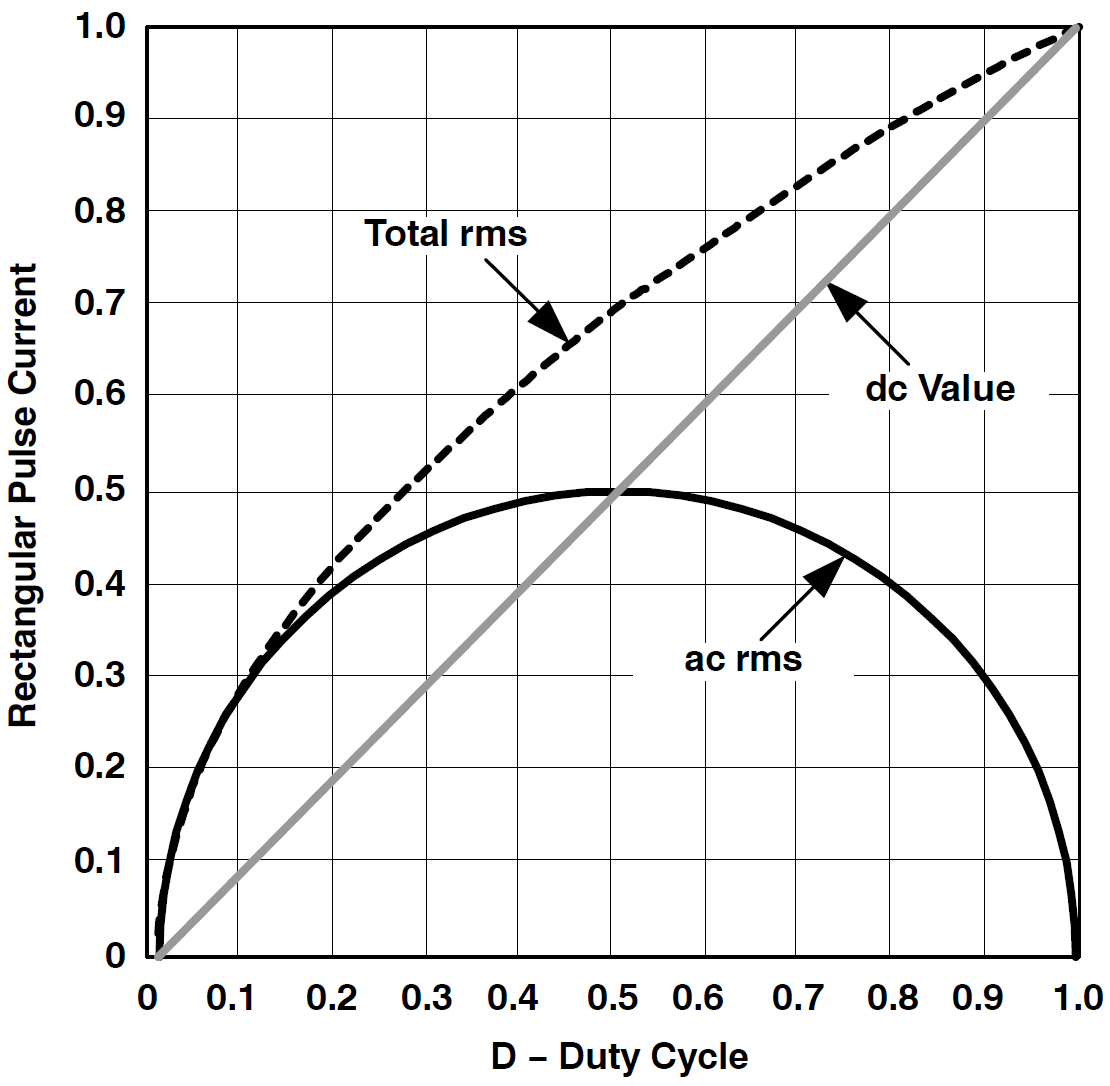
\includegraphics[width=0.8\linewidth]{fig/lec08/input_pulse_current_duty_cycle.png}
    \caption{Input pulse-current components versus duty cycle for a single-phase buck regulator. Adapted from Texas Instruments, \textit{Input and Output Capacitor Selection}, SLTA055}
\end{figure}
\end{column}
\end{columns}

\end{frame}


%%%%%%%%%%%%%%%%%%%%%%%%%%%%%%%%%%%%%%%%%%%%%%%%%%%%%%%%%%%%%
%% Input ceramic capacitance
%%%%%%%%%%%%%%%%%%%%%%%%%%%%%%%%%%%%%%%%%%%%%%%%%%%%%%%%%%%%%
\begin{frame}
\frametitle{Input Ceramic Capacitor Sizing}

\begin{columns}
\begin{column}{0.56\textwidth}
A first estimate of the required input ceramic capacitance for a buck regulator can be obtained from the allowable input ripple voltage. For a triangular charge-balance approximation,
\begin{align}
    C_{\mathrm{in,min}}
    \approx
    \frac{I_oD(1-D)}
    {f_s\Delta V_{\mathrm{in,pp}}}
\end{align}
where
\begin{itemize}
    \item \(I_o\) is the output load current,
    \item \(D\) is duty cycle,
    \item \(f_s\) is switching frequency,
    \item \(\Delta V_{\mathrm{in,pp}}\) is allowable peak-to-peak input ripple.
\end{itemize}
\end{column}

\begin{column}{0.40\textwidth}
\begin{block}{Important Practical Note}
\small
Texas Instruments recommends using the effective ceramic capacitance at operating DC voltage, not only the nominal datasheet value. In MLCCs, the effective capacitance can be much smaller than the rated value.
\end{block}
\end{column}
\end{columns}

\end{frame}


%%%%%%%%%%%%%%%%%%%%%%%%%%%%%%%%%%%%%%%%%%%%%%%%%%%%%%%%%%%%%
%% Input ceramic capacitance
%%%%%%%%%%%%%%%%%%%%%%%%%%%%%%%%%%%%%%%%%%%%%%%%%%%%%%%%%%%%%
\begin{frame}
\frametitle{Input Ceramic Capacitor Sizing}

\begin{columns}
\begin{column}{0.56\textwidth}

Important practical corrections:
\begin{itemize}
    \item use effective MLCC capacitance at DC bias,
    \item include temperature and tolerance,
    \item place capacitors close to the regulator input pins,
    \item minimize the high-frequency current loop.
\end{itemize}
\end{column}

\begin{column}{0.40\textwidth}

\begin{block}{Rule of Thumb}
\small
A small ripple target, such as tens of millivolts, can significantly reduce RMS ripple current flowing into the bulk capacitor.
\end{block}
\end{column}
\end{columns}

\end{frame}

%%%%%%%%%%%%%%%%%%%%%%%%%%%%%%%%%%%%%%%%%%%%%%%%%%%%%%%%%%%%%
%% Input capacitor placement
%%%%%%%%%%%%%%%%%%%%%%%%%%%%%%%%%%%%%%%%%%%%%%%%%%%%%%%%%%%%%
\begin{frame}
\frametitle{Input Capacitor Placement and Ripple Reduction}

\begin{columns}
\begin{column}{0.56\textwidth}

Input ceramic capacitors must be placed physically close to the converter input pins or switching devices. The reason is parasitic inductance: $Z_L = j\omega L_{\mathrm{par}}$.
Even a few nanohenries can significantly increase impedance at the switching frequency and its harmonics. Good placement achieves:
\begin{itemize}
    \item lower input ripple voltage,
    \item reduced RMS ripple current in bulk capacitors,
    \item lower EMI,
    \item reduced switching-loop ringing,
    \item lower stress on upstream supply cables.
\end{itemize}
\end{column}

\begin{column}{0.40\textwidth}
\begin{figure}
    \centering
    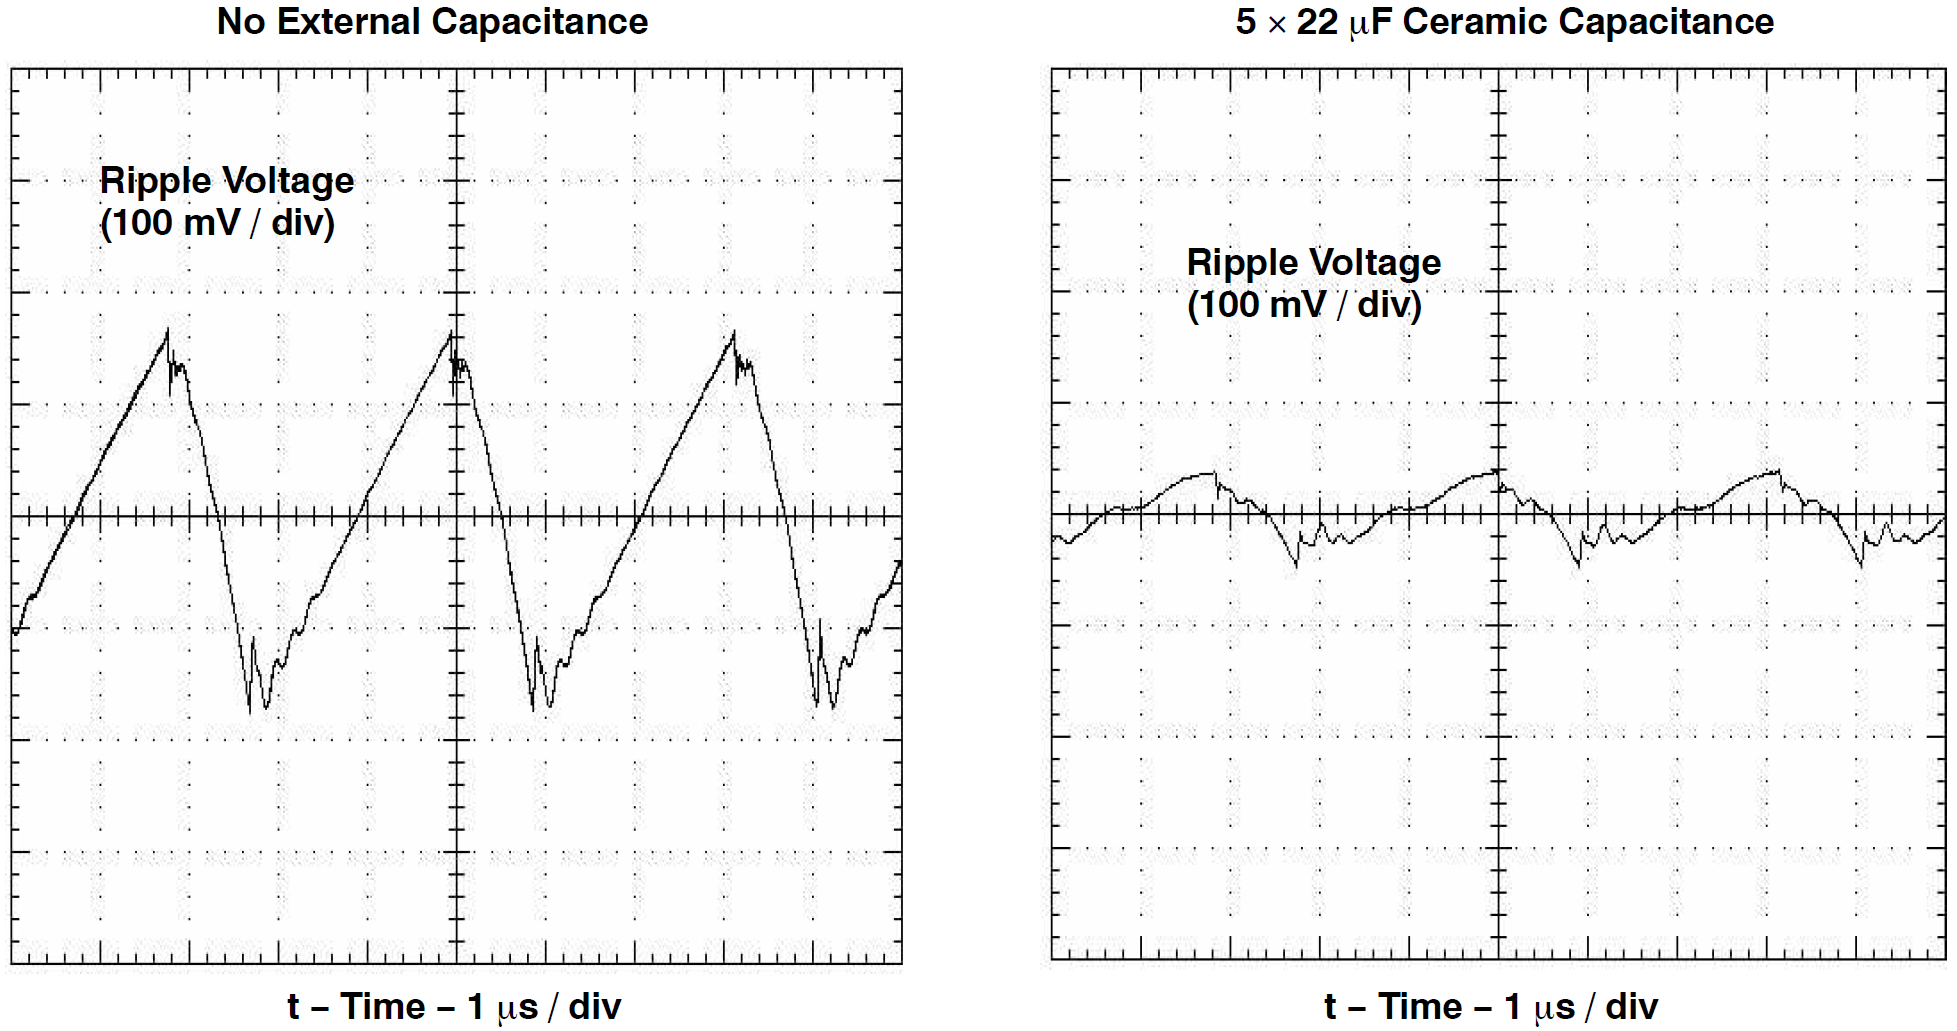
\includegraphics[width=\linewidth]{fig/lec08/input_ripple_voltage_plots.png}
    \caption{Input ripple-voltage reduction after adding ceramic input capacitors. Adapted from Texas Instruments, \textit{Input and Output Capacitor Selection}}
\end{figure}
\end{column}
\end{columns}
The bulk capacitor supports low-frequency energy demand; the local ceramic capacitor handles high-frequency switching current.
\end{frame}


%%%%%%%%%%%%%%%%%%%%%%%%%%%%%%%%%%%%%%%%%%%%%%%%%%%%%%%%%%%%%
%% Output capacitor function
%%%%%%%%%%%%%%%%%%%%%%%%%%%%%%%%%%%%%%%%%%%%%%%%%%%%%%%%%%%%%
\begin{frame}
\frametitle{Output Capacitor in a Buck Converter}

\begin{columns}
\begin{column}{0.56\textwidth}

The output capacitor reduces output-voltage ripple and supplies transient load current until the converter control loop and inductor current can respond. The output ripple contains several components:
\begin{align}
    \Delta v_o
    =
    \Delta v_C
    +
    \Delta v_{\mathrm{ESR}}
    +
    \Delta v_{\mathrm{ESL}}
\end{align}
where
\begin{itemize}
    \item \(\Delta v_C\) is due to charge/discharge of capacitance,
    \item \(\Delta v_{\mathrm{ESR}}\) is due to ripple current through ESR,
    \item \(\Delta v_{\mathrm{ESL}}\) is due to fast current transitions through ESL.
\end{itemize}
\end{column}

\begin{column}{0.40\textwidth}
\begin{figure}
    \centering
    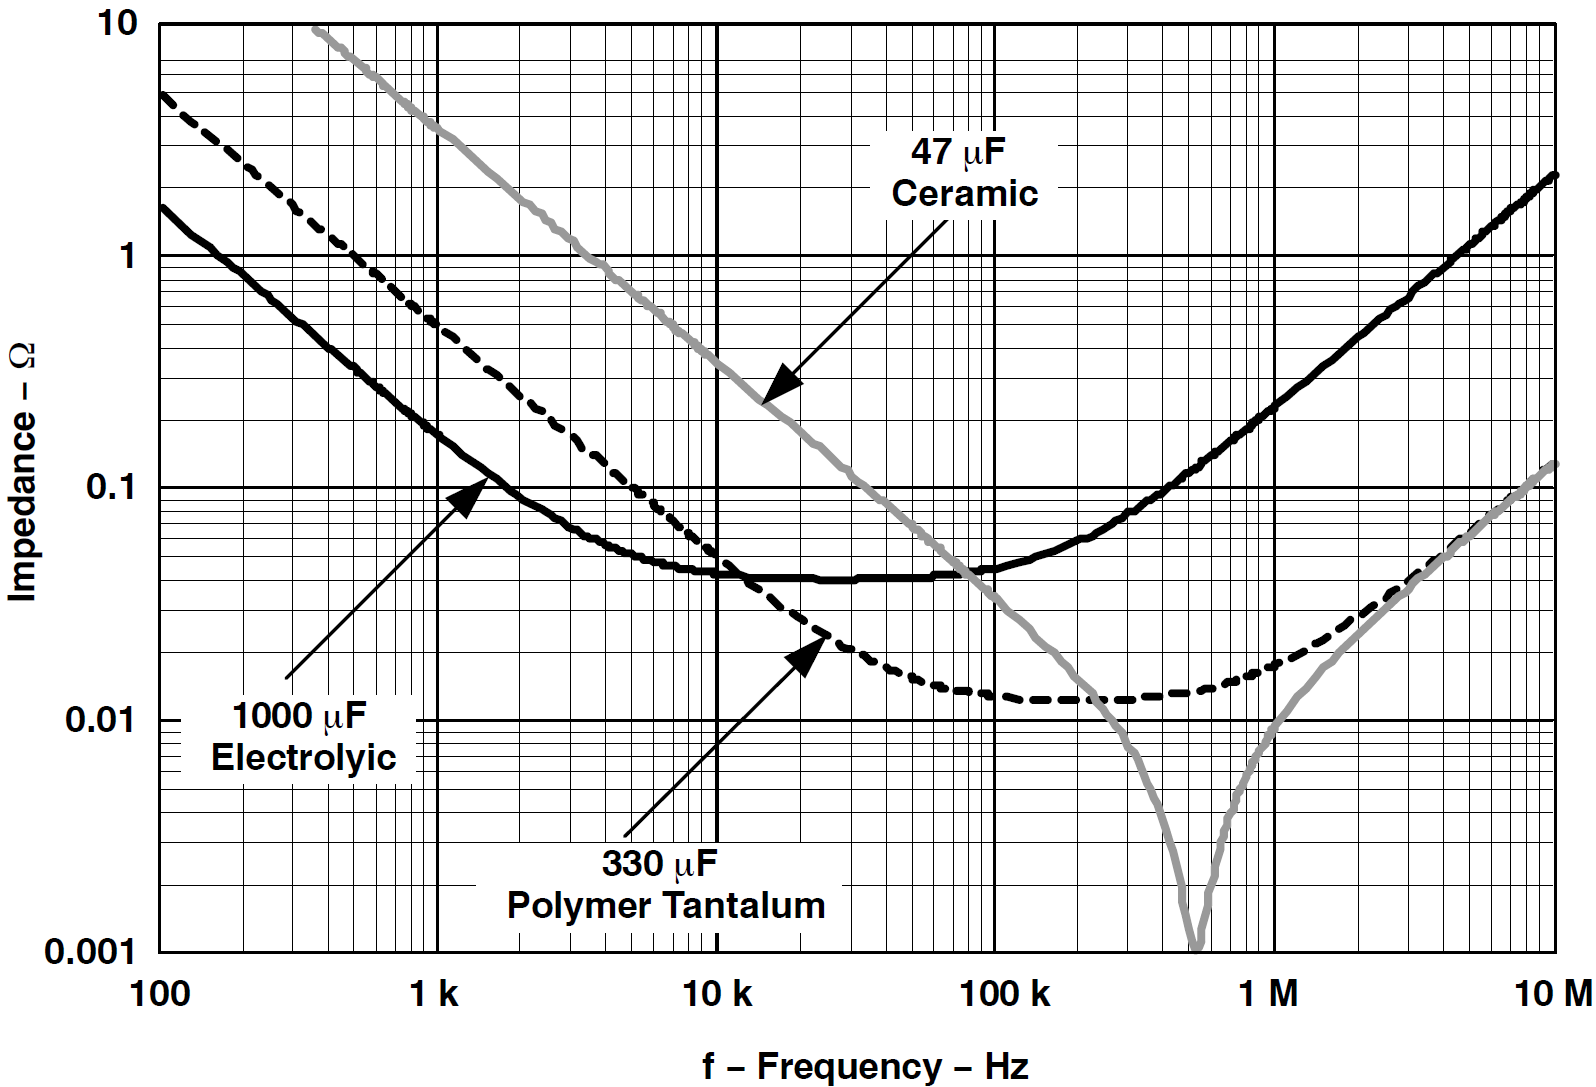
\includegraphics[width=\linewidth]{fig/lec08/capacitor_impedance_characteristics.png}
    \caption{Capacitor impedance characteristics relevant to output capacitor selection. Adapted from Texas Instruments, \textit{Input and Output Capacitor Selection}}
\end{figure}
\end{column}
\end{columns}

\end{frame}

%%%%%%%%%%%%%%%%%%%%%%%%%%%%%%%%%%%%%%%%%%%%%%%%%%%%%%%%%%%%%
%% Output capacitor function
%%%%%%%%%%%%%%%%%%%%%%%%%%%%%%%%%%%%%%%%%%%%%%%%%%%%%%%%%%%%%
\begin{frame}
\frametitle{Output Capacitor in a Buck Converter}

\begin{columns}
\begin{column}{0.56\textwidth}
For inductor ripple current \(\Delta i_L\), the ideal capacitive ripple is approximately
\begin{align}
    \Delta v_C
    \approx
    \frac{\Delta i_L}{8f_sC_o}
\end{align}
for a buck converter with triangular ripple current.
\end{column}

\begin{column}{0.40\textwidth}
\begin{figure}
    \centering
    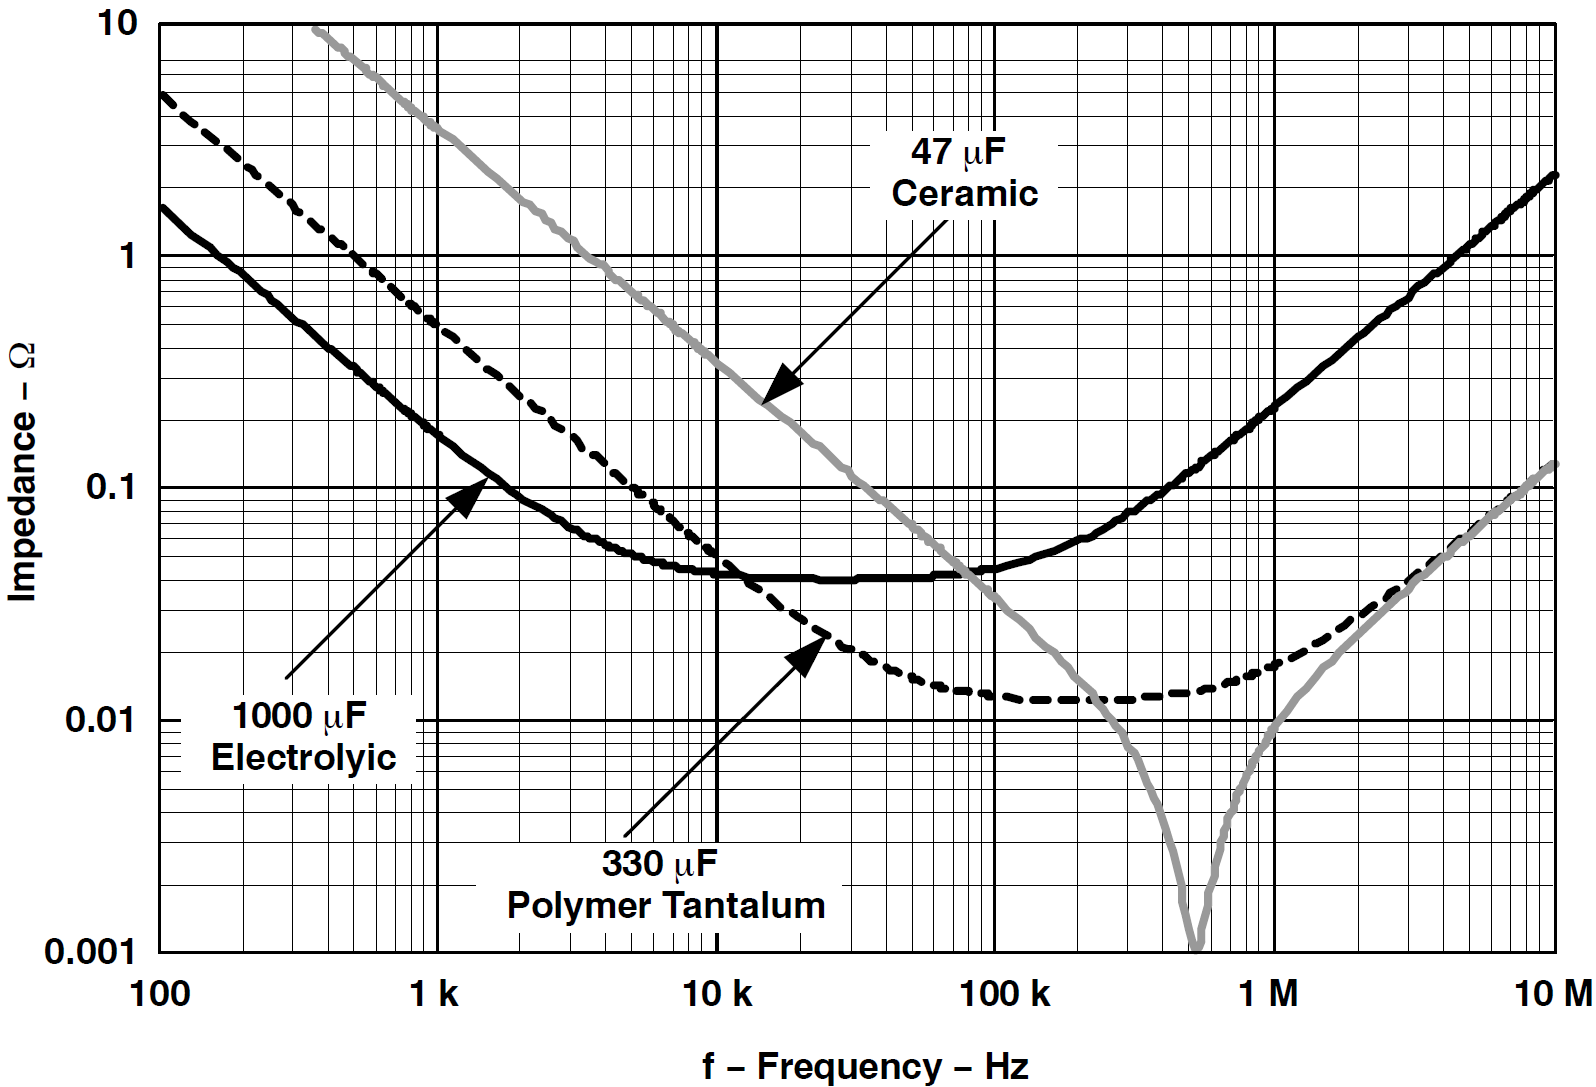
\includegraphics[width=\linewidth]{fig/lec08/capacitor_impedance_characteristics.png}
    \caption{Capacitor impedance characteristics relevant to output capacitor selection. Adapted from Texas Instruments, \textit{Input and Output Capacitor Selection}}
\end{figure}
\end{column}
\end{columns}

\end{frame}

%%%%%%%%%%%%%%%%%%%%%%%%%%%%%%%%%%%%%%%%%%%%%%%%%%%%%%%%%%%%%
%% Output capacitor load transient
%%%%%%%%%%%%%%%%%%%%%%%%%%%%%%%%%%%%%%%%%%%%%%%%%%%%%%%%%%%%%
\begin{frame}
\frametitle{Output Capacitor During Load Transients}
\begin{columns}
\begin{column}{0.56\textwidth}
During a sudden load-current increase, the converter inductor current cannot change instantaneously. The maximum inductor current slew rate is limited by
\begin{align}
    \frac{di_L}{dt}
    =
    \frac{\Delta V_L}{L}
\end{align}
Until the inductor current reaches the new load current, the current deficit must be supplied by the output capacitor. For a fast transient, the first voltage drop is often dominated by ESR:
\begin{align}
    \Delta V_{\mathrm{ESR}}
    =
    \Delta I_{\mathrm{load}} R_{\mathrm{ESR,eq}}
\end{align}
For slower transients, capacitance and control-loop response also contribute. Therefore, output capacitor design is a combination of impedance, capacitance, ESR, ESL, and control-loop bandwidth.
\end{column}

\begin{column}{0.40\textwidth}
\begin{figure}
    \centering
    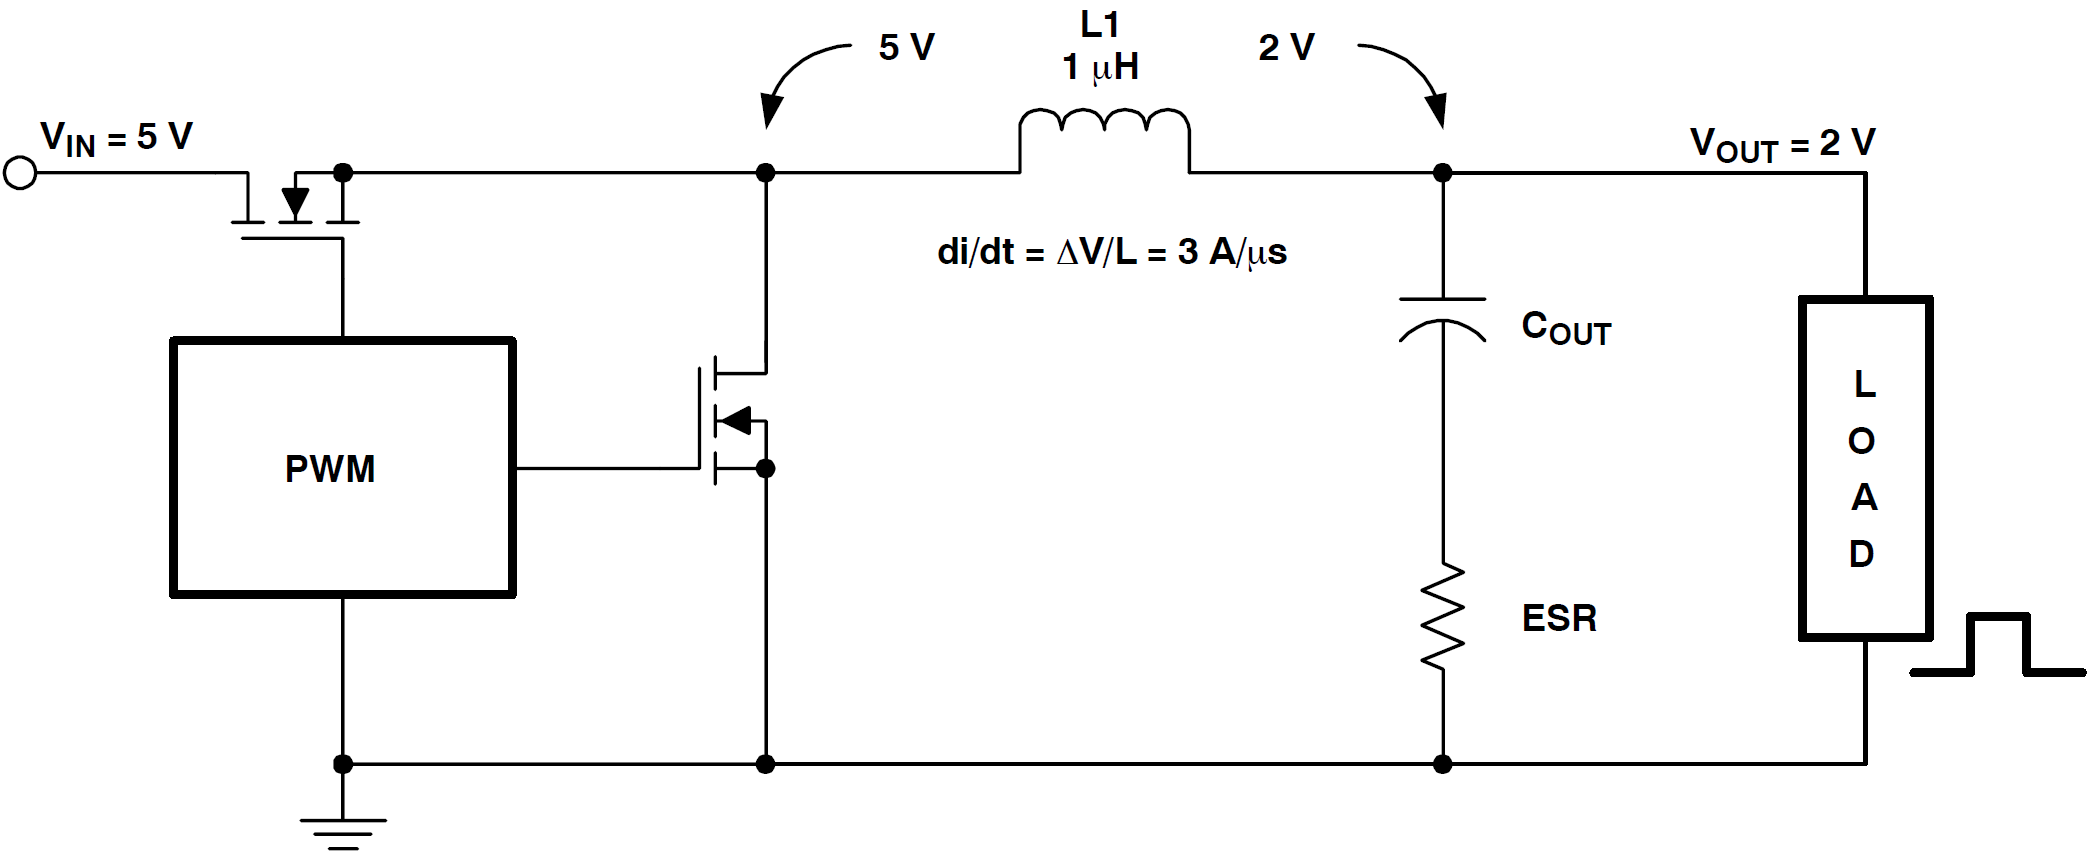
\includegraphics[width=\linewidth]{fig/lec08/regulator_slew_rate_example.png}
    \caption{Buck regulator slew-rate limitation during a load transient. Adapted from Texas Instruments, \textit{Input and Output Capacitor Selection}}
\end{figure}
\end{column}
\end{columns}

\end{frame}


%%%%%%%%%%%%%%%%%%%%%%%%%%%%%%%%%%%%%%%%%%%%%%%%%%%%%%%%%%%%%
%% Target impedance
%%%%%%%%%%%%%%%%%%%%%%%%%%%%%%%%%%%%%%%%%%%%%%%%%%%%%%%%%%%%%
\begin{frame}
\frametitle{Target Impedance for Output Capacitor Networks}
\begin{columns}
\begin{column}{0.56\textwidth}
A practical way to design output decoupling is the target-impedance method. For a maximum allowable transient voltage deviation \(\Delta V_{\max}\) and load step \(\Delta I_{\mathrm{load}}\),
\begin{align}
    Z_{\max}
    =
    \frac{\Delta V_{\max}}
    {\Delta I_{\mathrm{load}}}
\end{align}
The capacitor network should maintain
\begin{align}
    |Z_{\mathrm{out}}(j\omega)| < Z_{\max}
\end{align}
over the frequency range where the regulator cannot respond quickly enough. 
\end{column}

\begin{column}{0.40\textwidth}
\begin{figure}
    \centering
    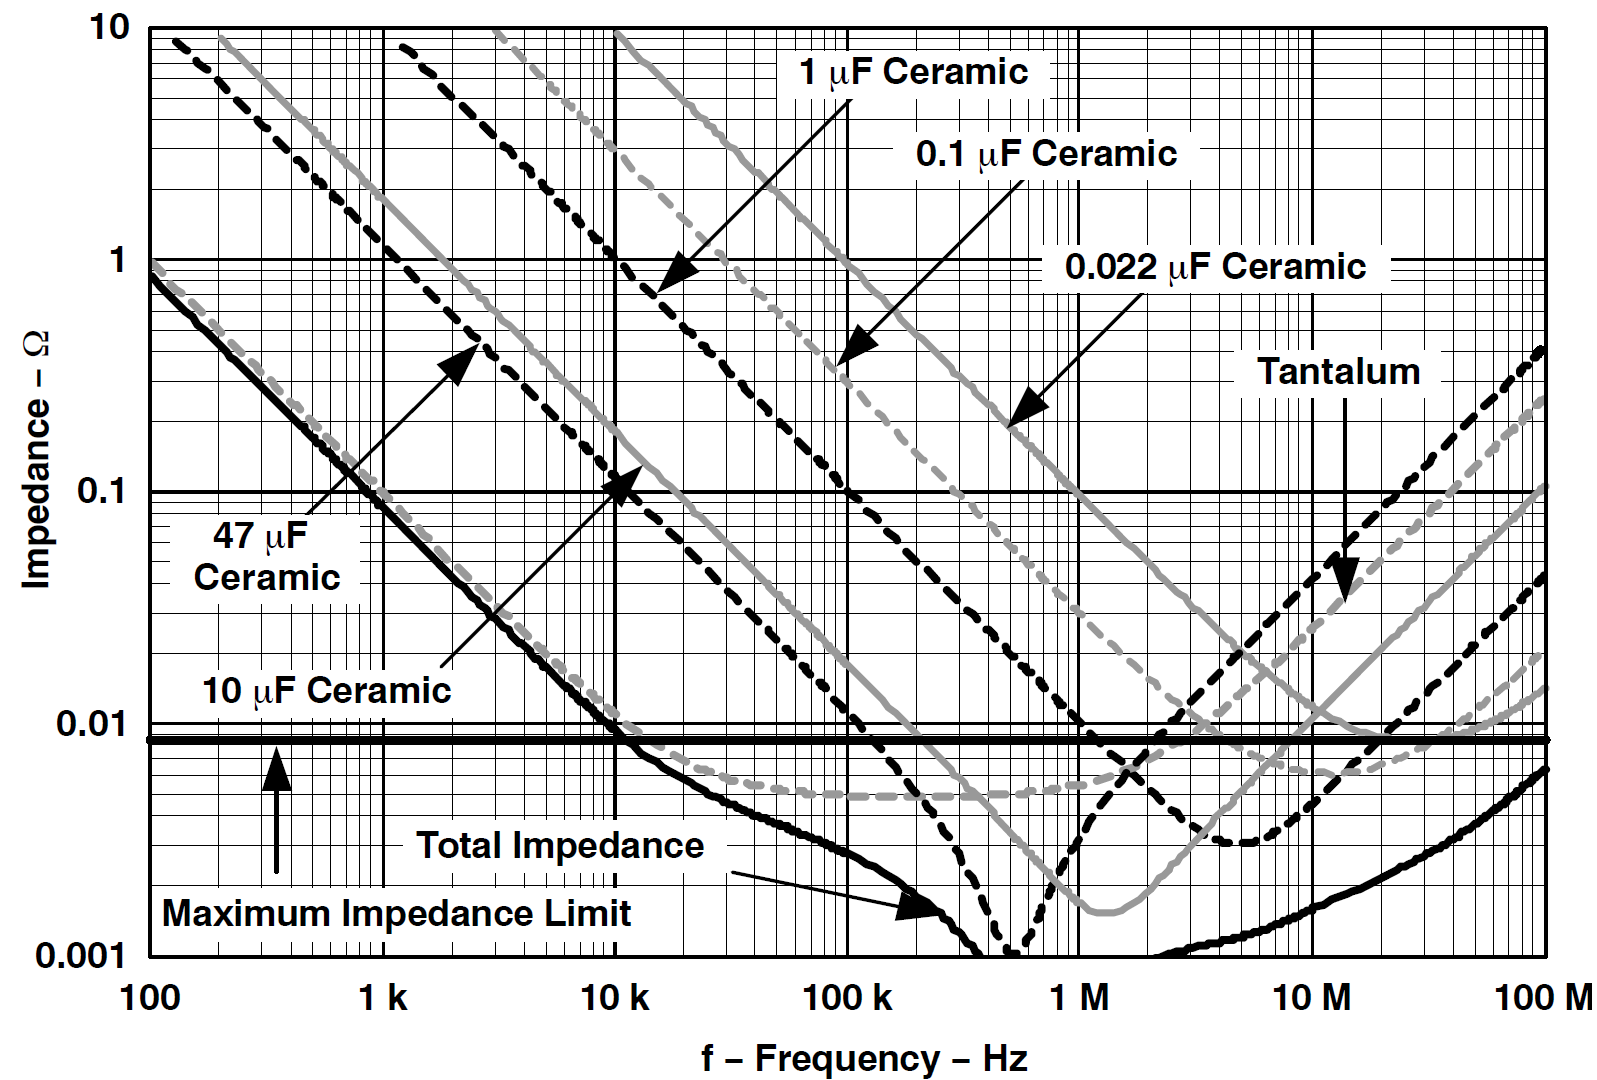
\includegraphics[width=\linewidth]{fig/lec08/high_frequency_impedance_plot.png}
    \caption{Output capacitor network impedance using multiple capacitor values and technologies. Adapted from Texas Instruments, \textit{Input and Output Capacitor Selection}}
\end{figure}
\end{column}
\end{columns}

\end{frame}


%%%%%%%%%%%%%%%%%%%%%%%%%%%%%%%%%%%%%%%%%%%%%%%%%%%%%%%%%%%%%
%% Target impedance
%%%%%%%%%%%%%%%%%%%%%%%%%%%%%%%%%%%%%%%%%%%%%%%%%%%%%%%%%%%%%
\begin{frame}
\frametitle{Target Impedance for Output Capacitor Networks}
\begin{columns}
\begin{column}{0.56\textwidth}
This usually requires several capacitor types:
\begin{itemize}
    \item bulk capacitor for low frequency,
    \item polymer or film capacitor for mid-frequency,
    \item MLCCs for high-frequency transients,
    \item very small MLCCs for MHz-range local decoupling.
\end{itemize}
\end{column}

\begin{column}{0.40\textwidth}
\begin{figure}
    \centering
    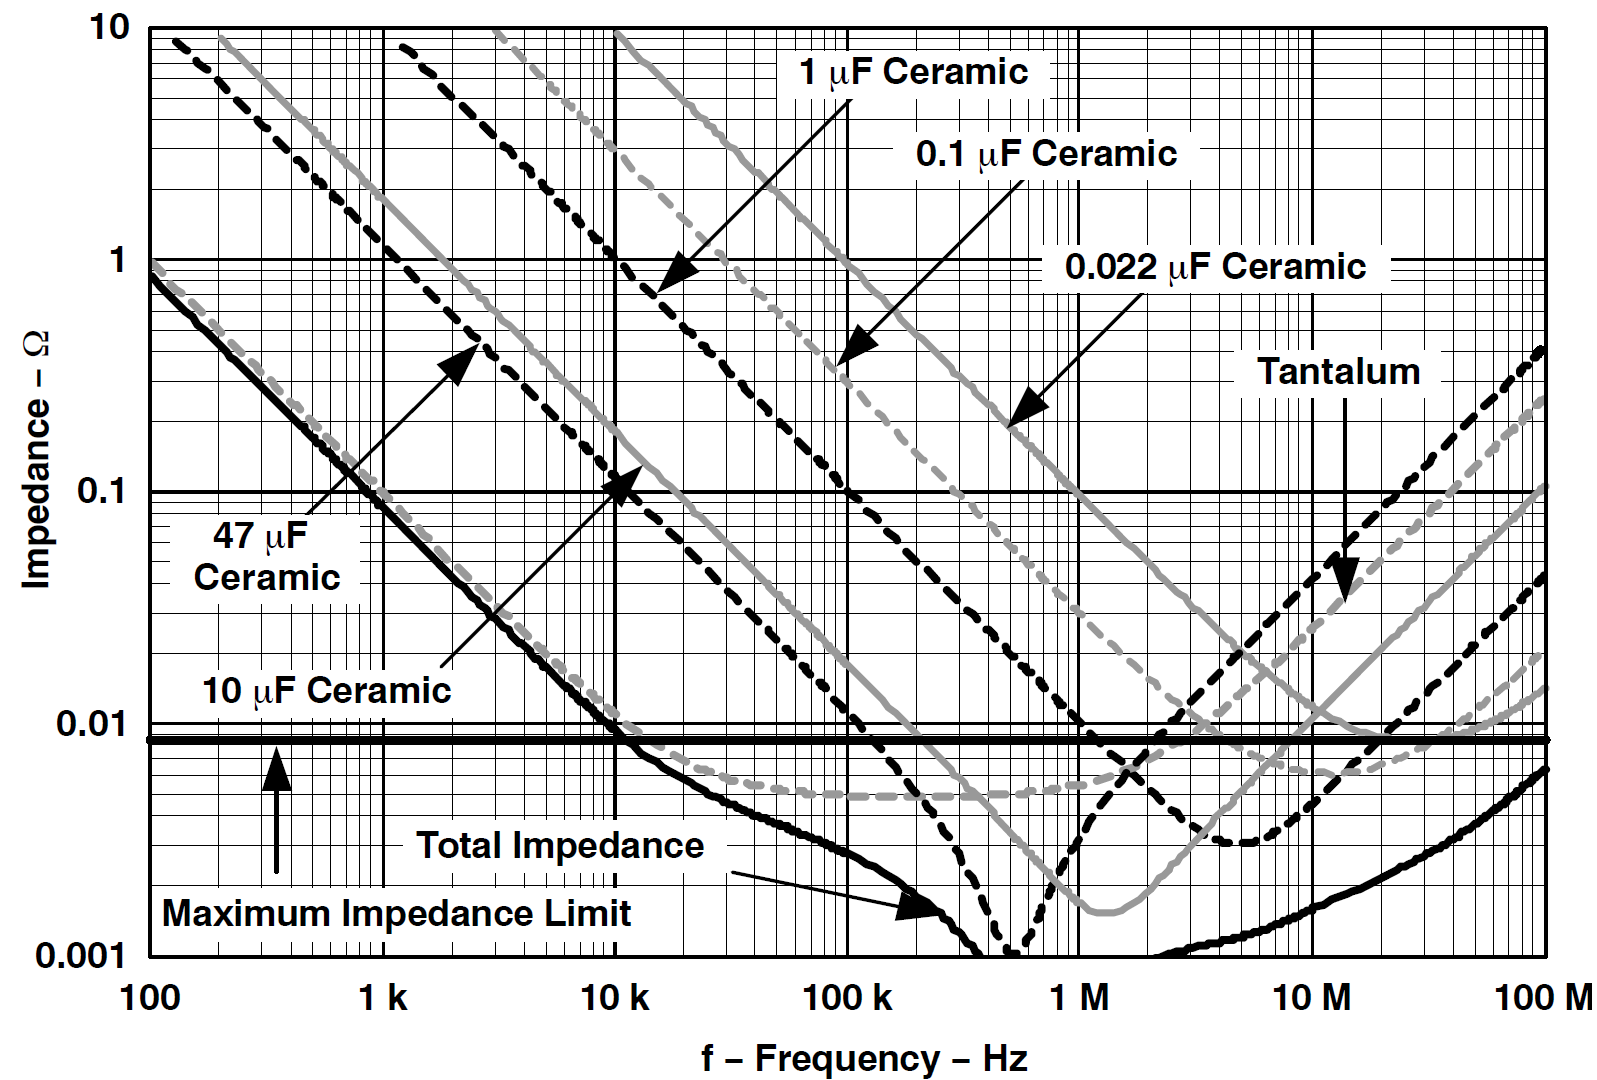
\includegraphics[width=\linewidth]{fig/lec08/high_frequency_impedance_plot.png}
    \caption{Output capacitor network impedance using multiple capacitor values and technologies. Adapted from Texas Instruments, \textit{Input and Output Capacitor Selection}}
\end{figure}
\end{column}
\end{columns}

\end{frame}
%%%%%%%%%%%%%%%%%%%%%%%%%%%%%%%%%%%%%%%%%%%%%%%%%%%%%%%%%%%%%
%% DC-link capacitor
%%%%%%%%%%%%%%%%%%%%%%%%%%%%%%%%%%%%%%%%%%%%%%%%%%%%%%%%%%%%%
\begin{frame}
\frametitle{DC-Link Capacitor}
\begin{columns}
\begin{column}{0.56\textwidth}
The DC-link capacitor is placed between two converter stages, for example between a rectifier and an inverter. Its main functions are:
\begin{itemize}
    \item balance instantaneous power between source and load,
    \item limit DC-bus voltage ripple,
    \item provide transient energy storage,
    \item reduce interaction between converter stages,
    \item provide a low-impedance path for switching ripple current.
\end{itemize}
\end{column}

\begin{column}{0.40\textwidth}
\begin{figure}
    \centering
    \vspace{-0.5cm}
    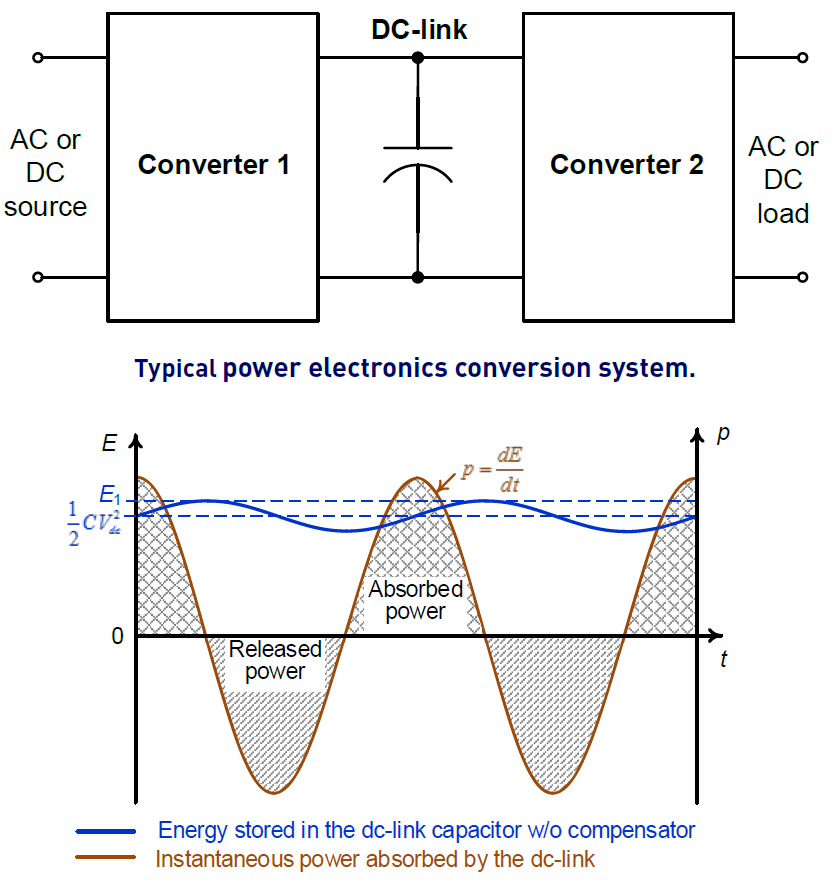
\includegraphics[width=0.75\linewidth]{fig/lec08/DC_link_function.png}
    \caption{Function of a capacitive DC link: power balancing, voltage-ripple limitation, and energy storage. Adapted from Huai Wang, \textit{Capacitors in Power Electronics Applications -- Reliability and Circuit Design}, IECON 2016 tutorial}
\end{figure}
\end{column}
\end{columns}
\end{frame}


%%%%%%%%%%%%%%%%%%%%%%%%%%%%%%%%%%%%%%%%%%%%%%%%%%%%%%%%%%%%%
%% DC-link capacitor
%%%%%%%%%%%%%%%%%%%%%%%%%%%%%%%%%%%%%%%%%%%%%%%%%%%%%%%%%%%%%
\begin{frame}
\frametitle{DC-Link Capacitor}
\begin{columns}
\begin{column}{0.56\textwidth}
The DC-link capacitor stored energy is
\begin{align}
    E_{\mathrm{dc}}
    =
    \frac{1}{2}C_{\mathrm{dc}}V_{\mathrm{dc}}^2
\end{align}
A small change in DC-link voltage corresponds to an energy change:
\begin{align}
    \Delta E
    =
    \frac{1}{2}C_{\mathrm{dc}}
    \left(
    V_{\max}^2 - V_{\min}^2
    \right)
\end{align}
\end{column}

\begin{column}{0.40\textwidth}
\begin{figure}
    \centering
    \vspace{-0.5cm}
    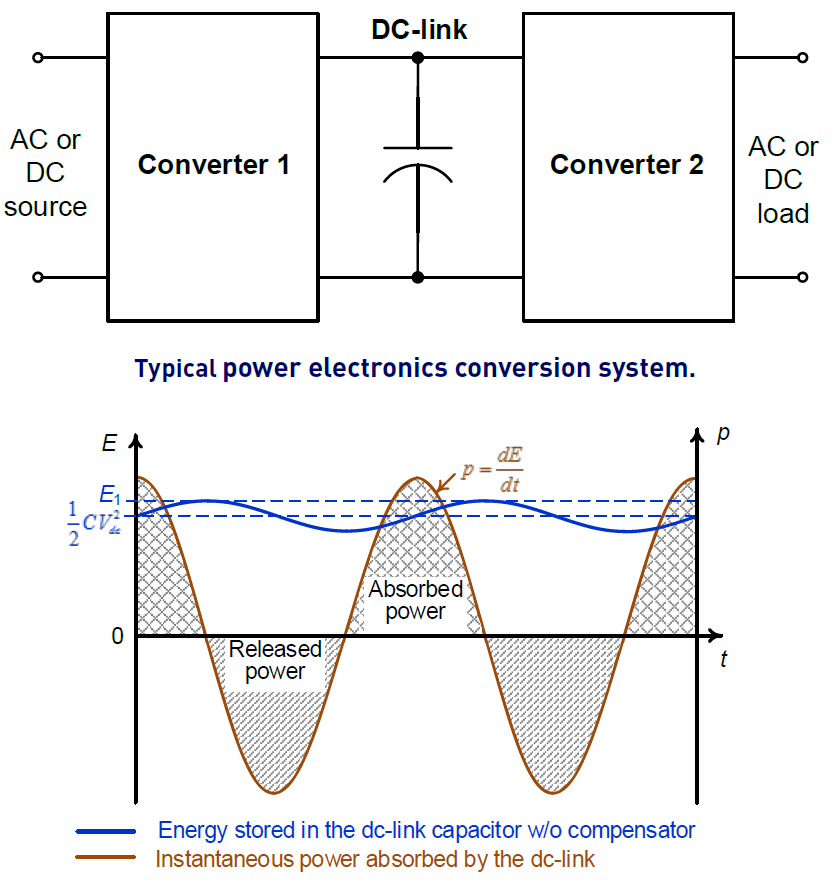
\includegraphics[width=0.75\linewidth]{fig/lec08/DC_link_function.png}
    \caption{Function of a capacitive DC link: power balancing, voltage-ripple limitation, and energy storage. Adapted from Huai Wang, \textit{Capacitors in Power Electronics Applications -- Reliability and Circuit Design}, IECON 2016 tutorial}
\end{figure}
\end{column}
\end{columns}
\end{frame}

%%%%%%%%%%%%%%%%%%%%%%%%%%%%%%%%%%%%%%%%%%%%%%%%%%%%%%%%%%%%%
%% DC-link capacitor in inverter
%%%%%%%%%%%%%%%%%%%%%%%%%%%%%%%%%%%%%%%%%%%%%%%%%%%%%%%%%%%%%
\begin{frame}
\frametitle{DC-Link Capacitor in Inverters and Motor Drives}
\begin{columns}
\begin{column}{0.56\textwidth}
In inverter systems, the DC-link capacitor is exposed to both low-frequency and high-frequency stress. Typical stress components include:
\begin{itemize}
    \item rectifier-side ripple,
    \item inverter switching ripple,
    \item load-dependent RMS ripple current,
    \item regenerative braking energy,
    \item overvoltage during load transients,
    \item thermal cycling from mission-profile variation.
\end{itemize}
\end{column}

\begin{column}{0.40\textwidth}
\begin{figure}
    \centering
    \vspace{-0.5cm}
    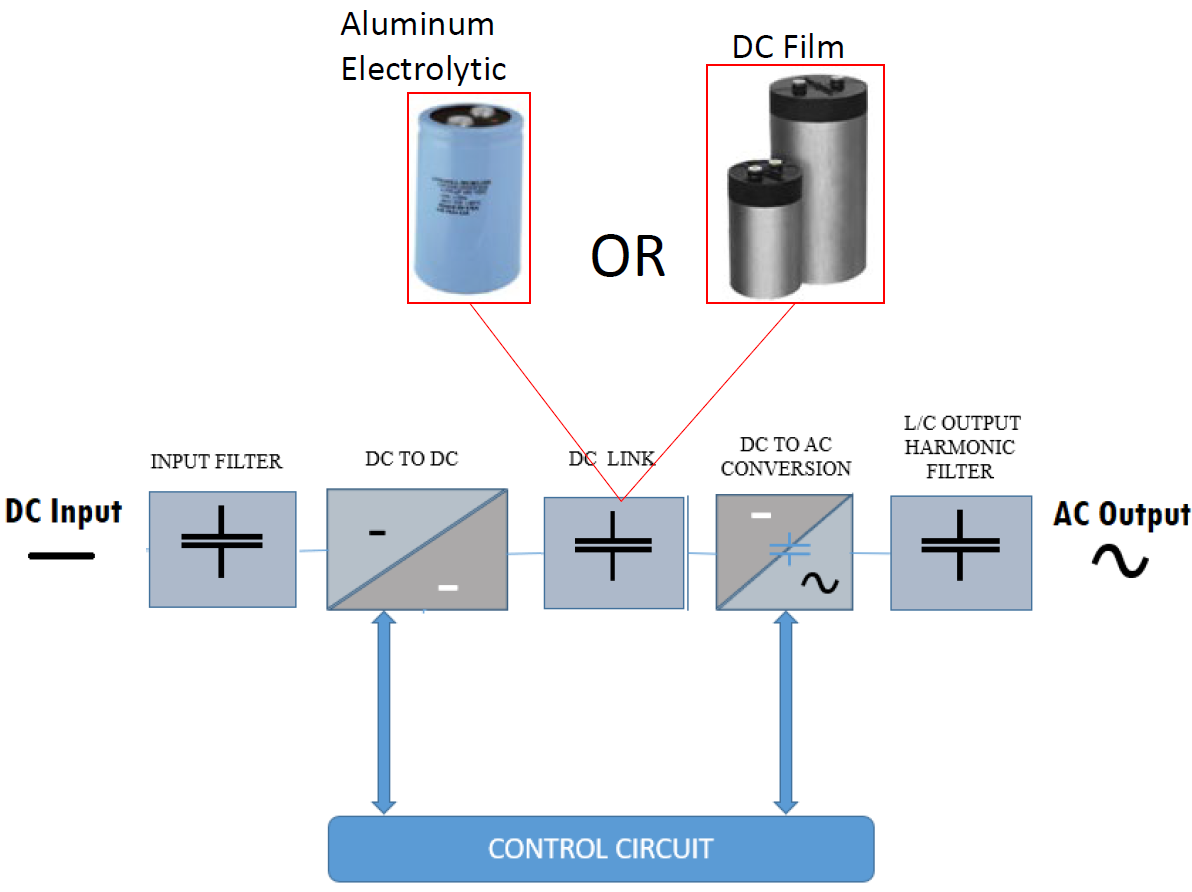
\includegraphics[width=\linewidth]{fig/lec08/DC_link_capacitors.png}
    \caption{DC-link capacitor location in a high-power inverter/converter system. Adapted from Cornell Dubilier, \textit{Capacitors for High Power Inverters and Converters}}
\end{figure}
\end{column}
\end{columns}

\end{frame}


%%%%%%%%%%%%%%%%%%%%%%%%%%%%%%%%%%%%%%%%%%%%%%%%%%%%%%%%%%%%%
%% DC-link capacitor in inverter
%%%%%%%%%%%%%%%%%%%%%%%%%%%%%%%%%%%%%%%%%%%%%%%%%%%%%%%%%%%%%
\begin{frame}
\frametitle{DC-Link Capacitor in Inverters and Motor Drives}
\begin{columns}
\begin{column}{0.56\textwidth}
For motor drives and grid converters, the DC-link capacitor is often one of the lifetime-critical components. Technology choice:
\begin{itemize}
    \item aluminum electrolytic: high capacitance and lower cost,
    \item film: higher ripple current, lower ESR, longer life, non-polar operation.
\end{itemize}
\end{column}

\begin{column}{0.40\textwidth}
\begin{figure}
    \centering
    \vspace{-0.5cm}
    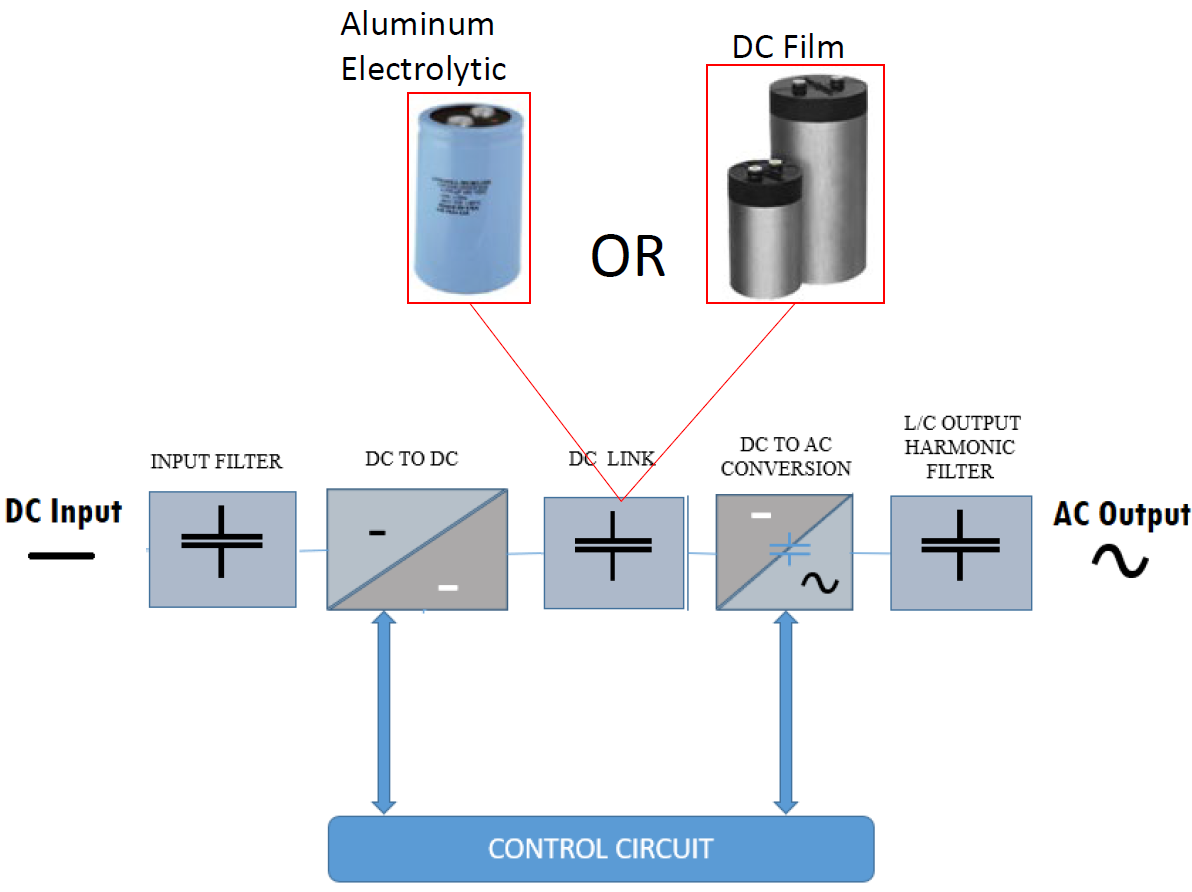
\includegraphics[width=\linewidth]{fig/lec08/DC_link_capacitors.png}
    \caption{DC-link capacitor location in a high-power inverter/converter system. Adapted from Cornell Dubilier, \textit{Capacitors for High Power Inverters and Converters}}
\end{figure}
\end{column}
\end{columns}

\end{frame}

%%%%%%%%%%%%%%%%%%%%%%%%%%%%%%%%%%%%%%%%%%%%%%%%%%%%%%%%%%%%%
%% Snubber capacitor
%%%%%%%%%%%%%%%%%%%%%%%%%%%%%%%%%%%%%%%%%%%%%%%%%%%%%%%%%%%%%
\begin{frame}
\frametitle{Snubber Capacitor}
\begin{columns}
\begin{column}{0.56\textwidth}
A snubber capacitor limits switching overvoltage caused by stray inductance:
\begin{align}
    v_{\mathrm{transient}}
    =
    L_{\sigma}\frac{di}{dt}
\end{align}
where \(L_{\sigma}\) is the commutation-loop stray inductance. It provides a local switching-current path and reduces device voltage rise. Key requirements:
\begin{itemize}
    \item low ESL,
    \item high pulse-current capability,
    \item high \(dv/dt\) rating,
    \item low loss at switching frequency,
    \item high voltage rating and surge capability.
\end{itemize}

\end{column}

\begin{column}{0.40\textwidth}
\begin{figure}
    \centering
    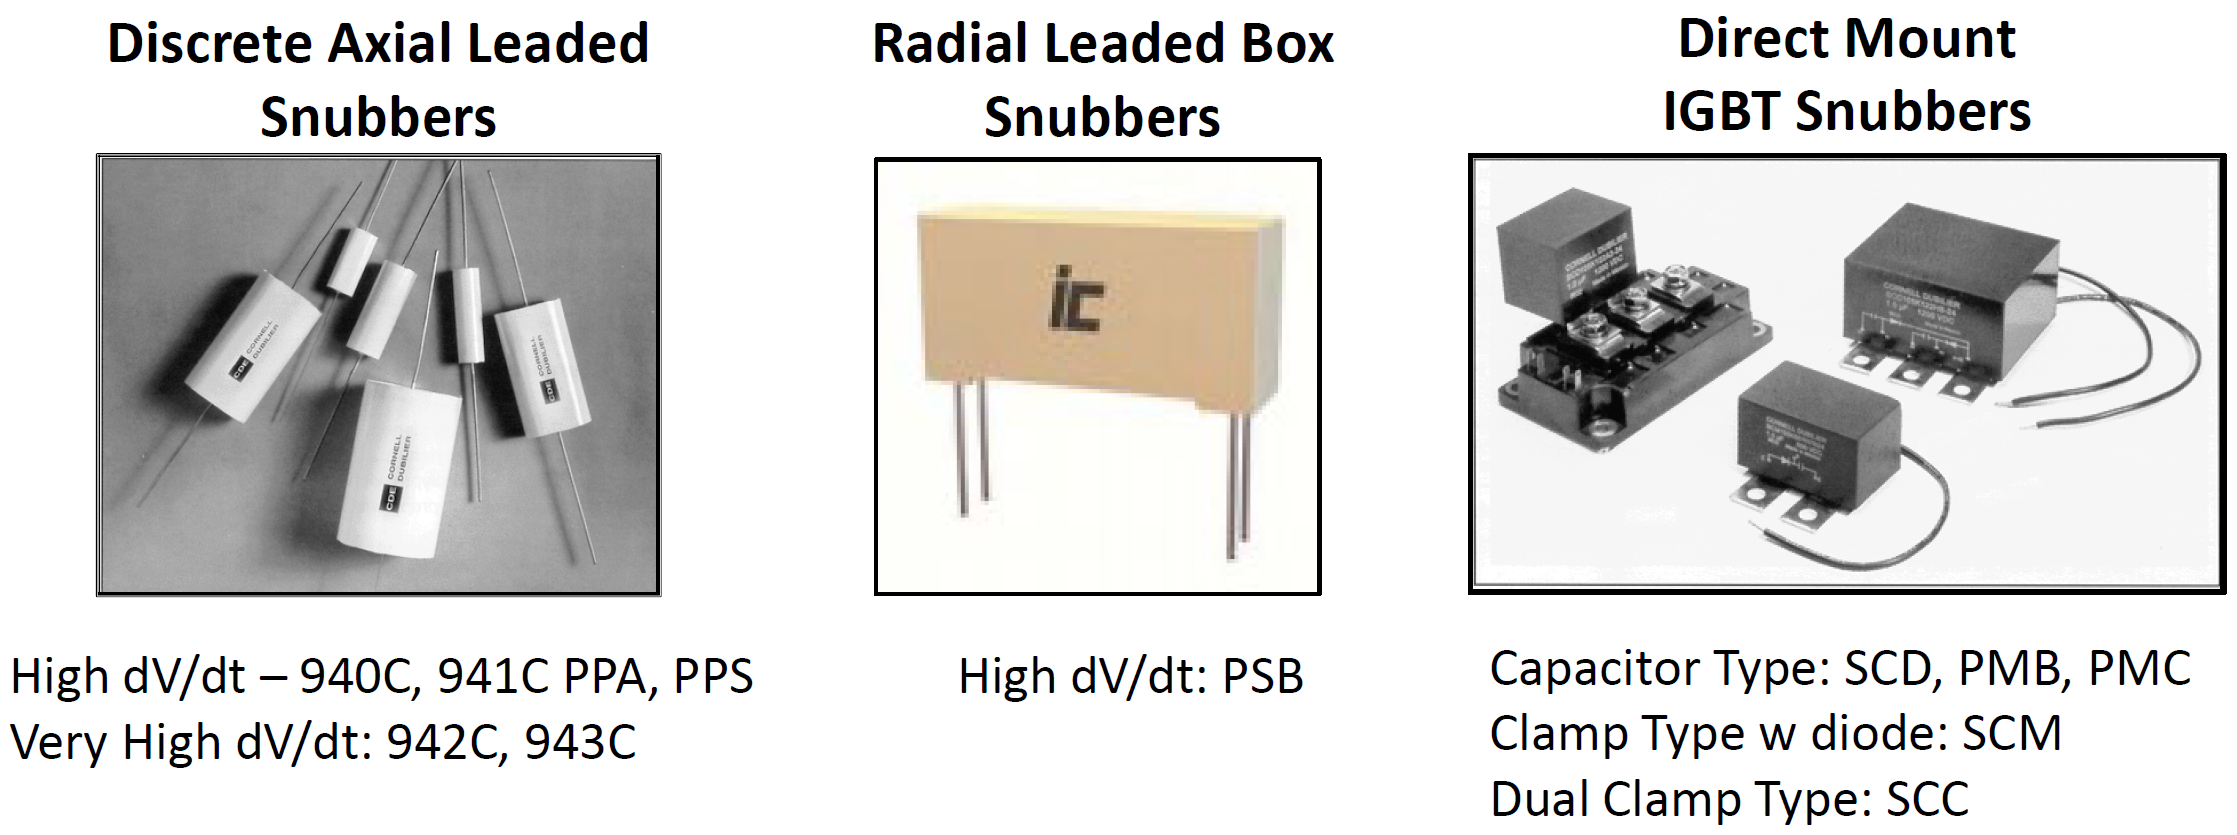
\includegraphics[width=\linewidth]{fig/lec08/snubber_definition_slide.png}
    \caption{Snubber concept: protection of switching devices from turn-off overvoltage caused by stray inductance and fast current change. Adapted from Cornell Dubilier, \textit{Capacitors for High Power Inverters and Converters}}
\end{figure}
\end{column}
\end{columns}

\end{frame}


%%%%%%%%%%%%%%%%%%%%%%%%%%%%%%%%%%%%%%%%%%%%%%%%%%%%%%%%%%%%%
%% Snubber voltage waveform
%%%%%%%%%%%%%%%%%%%%%%%%%%%%%%%%%%%%%%%%%%%%%%%%%%%%%%%%%%%%%
\begin{frame}
\frametitle{Snubber Capacitor Voltage Stress}
\begin{columns}
\begin{column}{0.56\textwidth}
Snubber capacitors require verification of voltage waveform, peak current, RMS current, and \(dv/dt\) rating. The capacitor current is
\begin{align}
    i_C = C\frac{dv_C}{dt}
\end{align}
High \(dv/dt\) produces high pulse current. For repetitive duty, verify:
\begin{itemize}
    \item maximum peak voltage,
    \item repetitive peak current,
    \item RMS current,
    \item pulse energy and thermal rise,
    \item permissible \(dv/dt\),
    \item mounting inductance.
\end{itemize}
\end{column}

\begin{column}{0.40\textwidth}
\begin{block}{Message}
Film capacitors are commonly used because of low loss, self-healing, and high pulse-current capability.
\end{block}
\begin{figure}
    \centering
    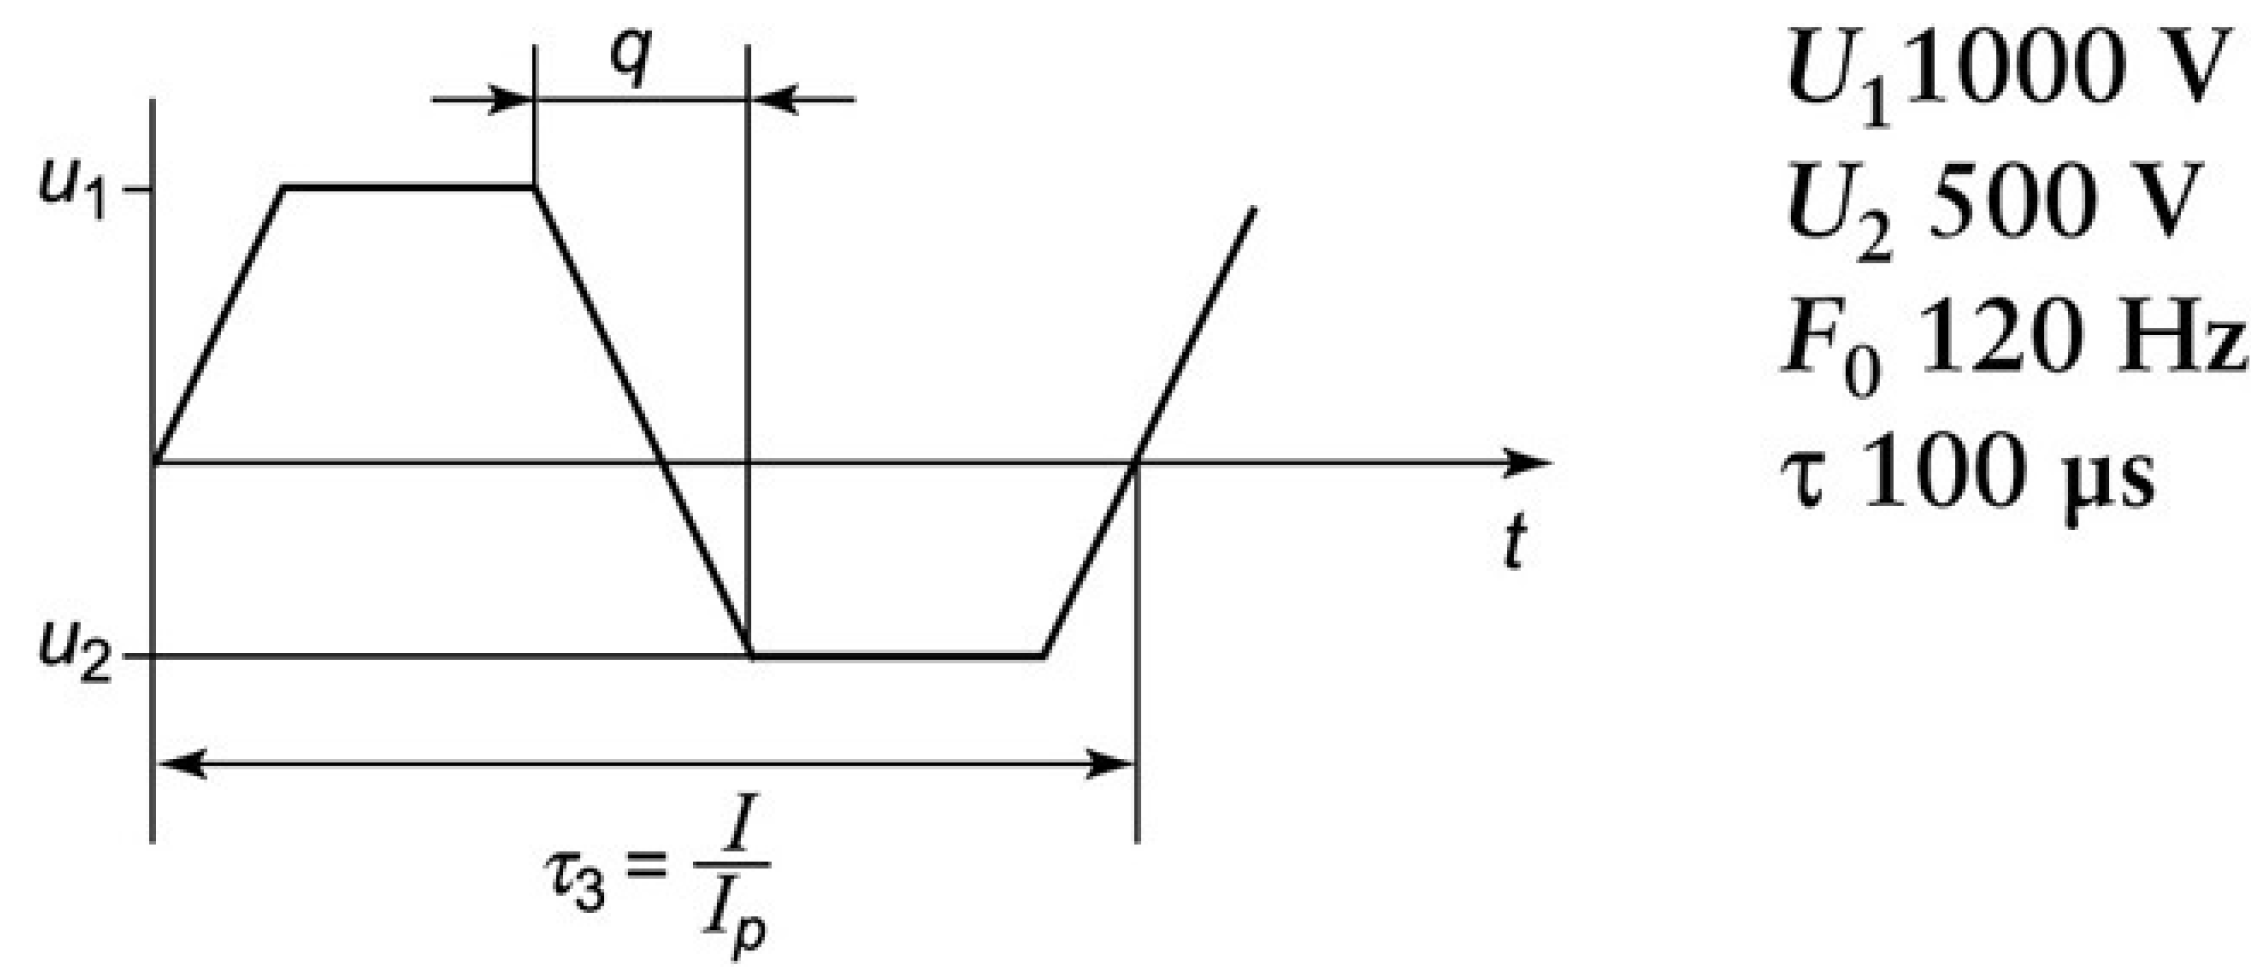
\includegraphics[width=\linewidth]{fig/lec08/snubber_turn_off_waveform.png}
    \caption{Turn-off voltage waveform used for snubber capacitor voltage-stress selection. Adapted from Deshpande, \textit{Capacitors} McGraw-Hill, 2015.}
\end{figure}
\end{column}
\end{columns}

\end{frame}


%%%%%%%%%%%%%%%%%%%%%%%%%%%%%%%%%%%%%%%%%%%%%%%%%%%%%%%%%%%%%
%% Resonant capacitor
%%%%%%%%%%%%%%%%%%%%%%%%%%%%%%%%%%%%%%%%%%%%%%%%%%%%%%%%%%%%%
\begin{frame}
\frametitle{Resonant Capacitor}
\begin{columns}
\begin{column}{0.56\textwidth}
In resonant converters, the capacitor is not only a filter element; it is part of the power-transfer mechanism. For an ideal series resonant tank,
\begin{align}
    f_r
    =
    \frac{1}{2\pi\sqrt{L_rC_r}}
\end{align}
The resonant capacitor must withstand:
\begin{itemize}
    \item high RMS current,
    \item sinusoidal or quasi-sinusoidal AC voltage,
    \item high reactive power circulation,
    \item frequency-dependent dielectric loss,
    \item capacitance tolerance and temperature drift.
\end{itemize}

\end{column}

\begin{column}{0.40\textwidth}
\centering
\begin{circuitikz}[scale=0.82, transform shape]
    \draw (0,0) to[sV,l=$v_{\mathrm{sw}}$] (0,-2.4)
          -- (4.2,-2.4)
          to[C,l=$C_r$] (4.2,-1.2)
          to[L,l=$L_r$] (4.2,0)
          -- (0,0);

    \draw[->, thick] (2.0,0.35) -- (3.4,0.35);
    \node at (2.7,0.68) {\small $i_r$};

    \node at (2.2,-3.0) {\small Simplified series resonant tank};
\end{circuitikz}

\begin{block}{Design Message}
In resonant converters, capacitor stability and loss directly affect resonant frequency, gain curve, circulating current, efficiency, and thermal stress.
\end{block}
\end{column}
\end{columns}
Typical technologies include polypropylene film capacitors, high-quality ceramic capacitors, and specialized resonant capacitors.
\end{frame}


%%%%%%%%%%%%%%%%%%%%%%%%%%%%%%%%%%%%%%%%%%%%%%%%%%%%%%%%%%%%%
%% AC harmonic filter capacitors
%%%%%%%%%%%%%%%%%%%%%%%%%%%%%%%%%%%%%%%%%%%%%%%%%%%%%%%%%%%%%
\begin{frame}
\frametitle{AC Harmonic Filter Capacitors}

\begin{columns}
\begin{column}{0.56\textwidth}
Inverters generate switching-frequency harmonics that must often be attenuated before the grid, motor, or load. AC harmonic filter capacitors are used together with inductors to form:
\begin{itemize}
    \item LC filters and LCL grid filters,
    \item tuned harmonic filters,
    \item motor-output sine filters,
    \item differential-mode EMI filters.
\end{itemize}
The capacitor must be selected for:
\begin{itemize}
    \item RMS voltage and current,
    \item harmonic current spectrum,
    \item dielectric loss and thermal rise,
    \item grid or motor-side overvoltage conditions.
\end{itemize}
\end{column}

\begin{column}{0.40\textwidth}
\begin{figure}
    \centering
    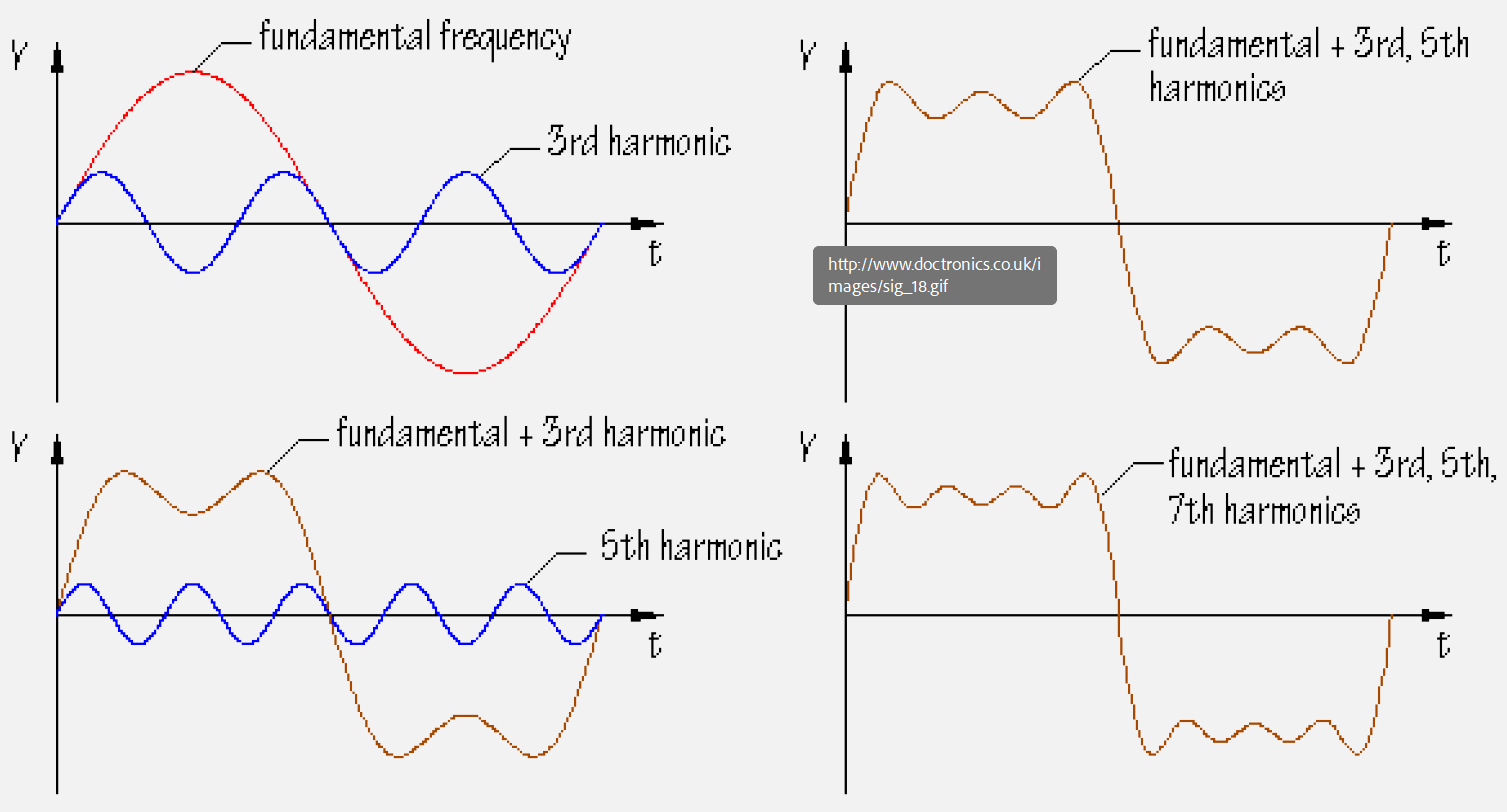
\includegraphics[width=\linewidth]{fig/lec08/AC_harmonic_filtering.png}
    \caption{Inverter switching harmonics and AC harmonic-filter capacitors used with tuned LC networks. Adapted from Cornell Dubilier, \textit{Capacitors for High Power Inverters and Converters}}
\end{figure}
\end{column}
\end{columns}
For AC use, non-polar film capacitors are commonly preferred.
\end{frame}


%%%%%%%%%%%%%%%%%%%%%%%%%%%%%%%%%%%%%%%%%%%%%%%%%%%%%%%%%%%%%
%% EMI and safety capacitors
%%%%%%%%%%%%%%%%%%%%%%%%%%%%%%%%%%%%%%%%%%%%%%%%%%%%%%%%%%%%%
\begin{frame}
\frametitle{EMI and Safety Capacitors}
\begin{columns}
\begin{column}{0.56\textwidth}
Capacitors used in EMI filters must satisfy both electrical and safety requirements.

\textbf{Y capacitors} are connected from line or DC rail to protective earth or chassis:
\begin{itemize}
    \item suppress common-mode noise,
    \item leakage current is safety-critical,
    \item capacitance value is limited by touch-current requirements.
\end{itemize}
\textbf{Y capacitors} are connected from line or DC rail to protective earth or chassis:
\begin{itemize}
    \item suppress common-mode noise,
    \item leakage current is safety-critical,
    \item capacitance value is limited by touch-current requirements.
\end{itemize}
\end{column}

\begin{column}{0.40\textwidth}
\begin{center}
\begin{circuitikz}[scale=0.83, transform shape]
    \draw (0,0) node[left]{L} -- (4,0);
    \draw (0,-1.2) node[left]{N} -- (4,-1.2);
    \draw (0,-2.4) node[left]{PE} -- (4,-2.4);

    \draw (1.3,0) to[C,l=$C_X$] (1.3,-1.2);
    \draw (2.7,0) to[C,l=$C_Y$] (2.7,-2.4);
    \draw (3.5,-1.2) to[C,l=$C_Y$] (3.5,-2.4);

    \node at (2.0,0.45) {\small EMI filter capacitors};
\end{circuitikz}
\end{center}
\end{column}
\end{columns}
\end{frame}



%%%%%%%%%%%%%%%%%%%%%%%%%%%%%%%%%%%%%%%%%%%%%%%%%%%%%%%%%%%%%
%% EMI and safety capacitors
%%%%%%%%%%%%%%%%%%%%%%%%%%%%%%%%%%%%%%%%%%%%%%%%%%%%%%%%%%%%%
\begin{frame}
\frametitle{EMI and Safety Capacitors}
\begin{columns}
\begin{column}{0.56\textwidth}
EMI capacitors are therefore selected not only by capacitance and voltage, but also by safety class, impulse rating, leakage current, and insulation requirements.
\end{column}

\begin{column}{0.40\textwidth}
\begin{figure}
    \centering
    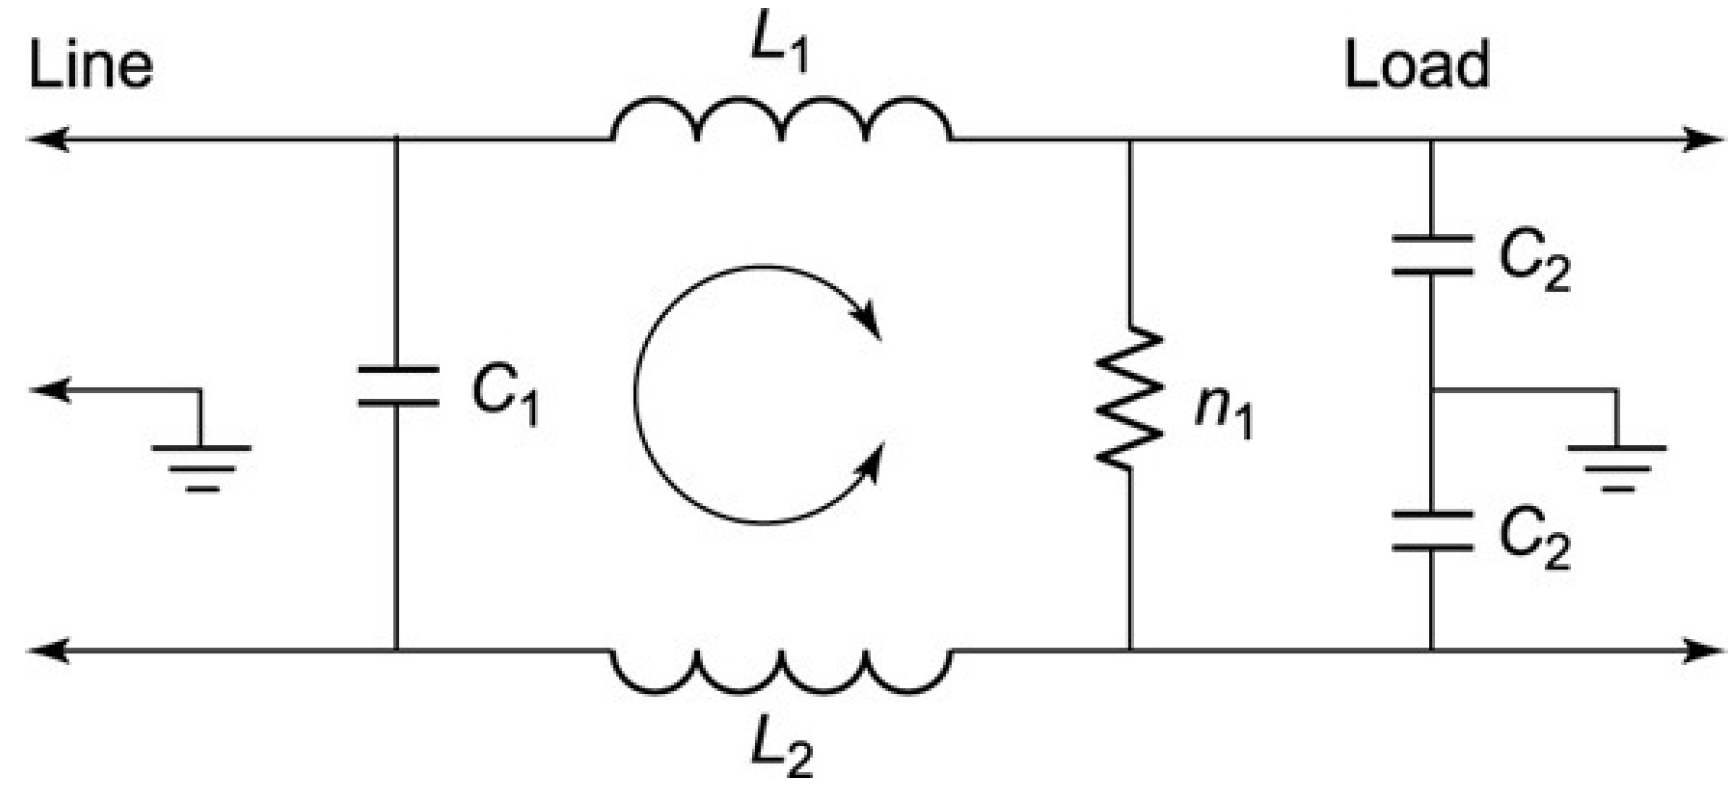
\includegraphics[width=\linewidth]{fig/lec08/XY_capacitors.png}
    \caption{X and Y capacitors used in EMI filters. Adapted from Deshpande, \textit{Capacitors} McGraw-Hill, 2015.}
\end{figure}

\end{column}
\end{columns}
\end{frame}

%%%%%%%%%%%%%%%%%%%%%%%%%%%%%%%%%%%%%%%%%%%%%%%%%%%%%%%%%%%%%
%% Summary of capacitor applications
%%%%%%%%%%%%%%%%%%%%%%%%%%%%%%%%%%%%%%%%%%%%%%%%%%%%%%%%%%%%%
\begin{frame}
\frametitle{Summary: Capacitor Functions in Converters}

\scriptsize
\begin{table}
\centering
\begin{tabular}{p{0.20\textwidth}p{0.25\textwidth}p{0.22\textwidth}p{0.22\textwidth}}
\hline
\textbf{Application} & \textbf{Main Function} & \textbf{Dominant Stress} & \textbf{Typical Technology}\\
\hline
Input capacitor &
Reduce source ripple and supply pulsed current &
High-frequency RMS current, ESL &
MLCC, polymer, electrolytic, film\\

Output capacitor &
Reduce ripple and support load transients &
Target impedance, ESR, transient current &
MLCC, polymer, electrolytic\\

DC-link capacitor &
Energy buffer and DC-bus stabilization &
RMS ripple current, voltage, lifetime &
Film, electrolytic, hybrid banks\\

Snubber capacitor &
Limit switching overvoltage &
High \(dv/dt\), peak current, ESL &
Film, ceramic, power ceramic\\

Resonant capacitor &
Define resonant frequency and transfer power &
High RMS current, low loss, stability &
Polypropylene film, ceramic\\

AC/EMI filter capacitor &
Suppress harmonics and noise &
AC RMS voltage/current, safety &
Film, X/Y safety capacitors\\
\hline
\end{tabular}
\end{table}

\vspace{0.15cm}

\begin{block}{Message}
\small
The capacitor function determines the dominant design constraint. Therefore, the same nominal capacitance value may be suitable in one converter position and completely unsuitable in another.
\end{block}

\end{frame}


%%%%%%%%%%%%%%%%%%%%%%%%%%%%%%%%%%%%%%%%%%%%%%%%%%%%%%%%%%%%%
%% Capacitor sizing and selection methodology
%%%%%%%%%%%%%%%%%%%%%%%%%%%%%%%%%%%%%%%%%%%%%%%%%%%%%%%%%%%%%
\begin{frame}
\begin{center}
  \textbf{\Huge{Capacitor Sizing and Selection}}\\[0.4cm]
  \textbf{\Large{Voltage, Capacitance, Ripple Current, Losses, Temperature, and Layout}}
\end{center}
\end{frame}


%%%%%%%%%%%%%%%%%%%%%%%%%%%%%%%%%%%%%%%%%%%%%%%%%%%%%%%%%%%%%
%% Capacitor selection workflow
%%%%%%%%%%%%%%%%%%%%%%%%%%%%%%%%%%%%%%%%%%%%%%%%%%%%%%%%%%%%%
\begin{frame}
\frametitle{Capacitor Selection Workflow}

\begin{columns}
\begin{column}{0.56\textwidth}
Capacitor selection in power electronics should follow a systematic procedure. The nominal capacitance is only one part of the design. A practical workflow is:

\begin{enumerate}
    \item Define the capacitor function.
    \item Select voltage rating and derating.
    \item Determine required capacitance.
    \item Check RMS and peak current.
    \item Estimate losses and temperature rise.
    \item Verify ESR, ESL and resonance.
    \item Check lifetime and end-of-life limits.
    \item Validate layout, cooling and mechanical mounting.
\end{enumerate}
The final capacitor is acceptable only if all electrical, thermal, reliability and layout constraints are simultaneously satisfied.
\end{column}

\begin{column}{0.40\textwidth}
\begin{figure}
    \centering
    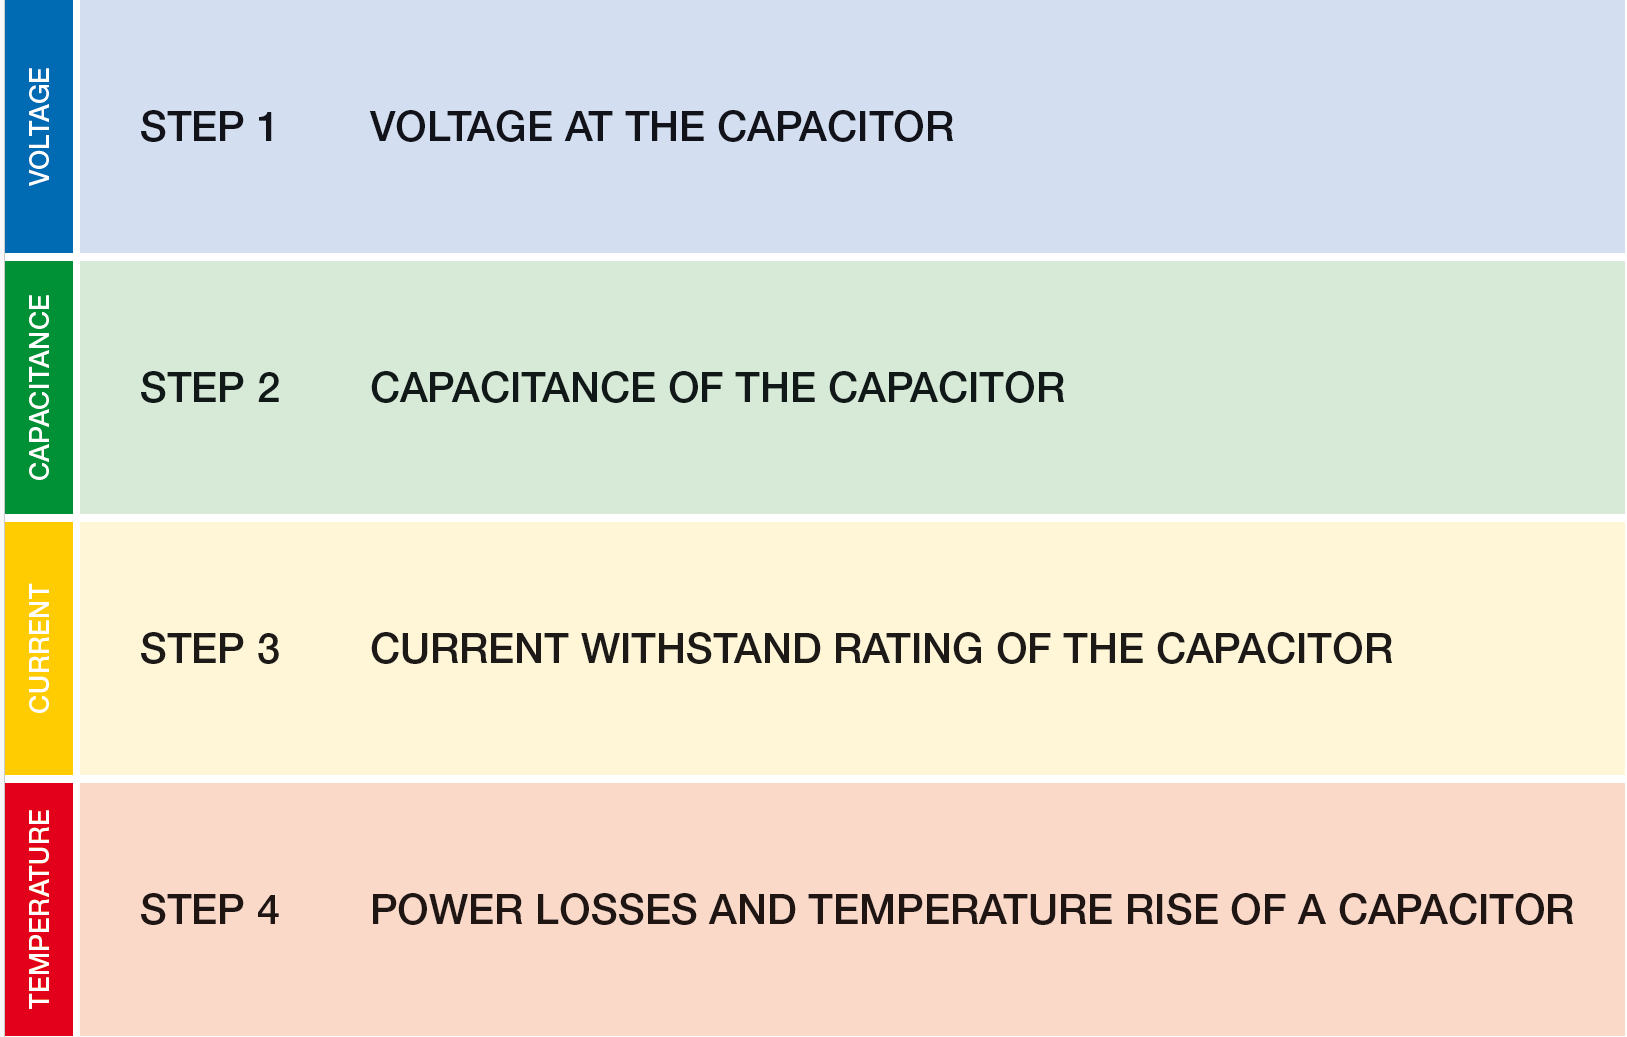
\includegraphics[width=\linewidth]{fig/lec08/selection_steps.png}
    \caption{Four-step selection procedure: voltage, capacitance, current withstand, and power-loss/temperature-rise verification. Adapted from FRAKO, \textit{Power Electronics Capacitors Selection Guide}}
\end{figure}
\end{column}
\end{columns}

\end{frame}


%%%%%%%%%%%%%%%%%%%%%%%%%%%%%%%%%%%%%%%%%%%%%%%%%%%%%%%%%%%%%
%% Selection workflow using circuitikz
%%%%%%%%%%%%%%%%%%%%%%%%%%%%%%%%%%%%%%%%%%%%%%%%%%%%%%%%%%%%%
\begin{frame}
\frametitle{Engineering Workflow for Capacitor Selection}

\begin{center}
\begin{circuitikz}[scale=0.73, transform shape]
    \tikzstyle{block} = [draw, rounded corners, align=center,
    minimum width=2.7cm, minimum height=0.75cm, font=\scriptsize]

    \node[block] (app) at (0,0) {Application\\function};
    \node[block] (volt) at (3.3,0) {Voltage rating\\and derating};
    \node[block] (cap) at (6.6,0) {Capacitance\\requirement};
    \node[block] (curr) at (9.9,0) {RMS and peak\\current rating};

    \node[block] (loss) at (9.9,-2.0) {Loss and\\temperature rise};
    \node[block] (imp) at (6.6,-2.0) {ESR, ESL and\\resonance};
    \node[block] (life) at (3.3,-2.0) {Lifetime and\\end-of-life};
    \node[block] (layout) at (0,-2.0) {Layout, cooling\\and mounting};

    \node[block, minimum width=3.2cm] (valid) at (4.95,-4.0) {Prototype, measurement\\and iteration};

    \draw[->, thick] (app) -- (volt);
    \draw[->, thick] (volt) -- (cap);
    \draw[->, thick] (cap) -- (curr);
    \draw[->, thick] (curr) -- (loss);
    \draw[->, thick] (loss) -- (imp);
    \draw[->, thick] (imp) -- (life);
    \draw[->, thick] (life) -- (layout);
    \draw[->, thick] (layout) -- (valid);

    \draw[->, thick, dashed] (valid.north) .. controls (4.95,-1.0) and (1.5,-1.0) .. (app.south);
\end{circuitikz}
\end{center}

\begin{block}{Message}
\small
Capacitor selection is iterative. Increasing capacitance may reduce voltage ripple, but it can increase volume, cost, inrush current and stored energy. Reducing ESR may improve heating, but layout ESL can still dominate high-frequency behaviour.
\end{block}

\end{frame}


%%%%%%%%%%%%%%%%%%%%%%%%%%%%%%%%%%%%%%%%%%%%%%%%%%%%%%%%%%%%%
%% Voltage rating and derating
%%%%%%%%%%%%%%%%%%%%%%%%%%%%%%%%%%%%%%%%%%%%%%%%%%%%%%%%%%%%%
\begin{frame}
\frametitle{Step 1: Voltage Rating and Derating}
The voltage rating must be selected from the worst-case voltage appearing at the capacitor terminals. The designer should consider:
\begin{itemize}
    \item nominal DC voltage and RMS AC voltage,
    \item peak repetitive voltage,
    \item switching overvoltage,
    \item surge voltage,
    \item regenerative or abnormal operating conditions,
    \item lifetime derating.
\end{itemize}
For DC operation,
\begin{align}
    V_{\mathrm{rated}} > V_{\mathrm{dc,max}}
\end{align}
For AC operation, the rated voltage must exceed the peak of the applied AC waveform:
\begin{align}
    V_{\mathrm{rated}} > V_{\mathrm{pk}}
\end{align}
In PWM filter applications, the capacitor peak voltage can be higher than the inverter DC-bus voltage due to switching and resonance effects.
\end{frame}


%%%%%%%%%%%%%%%%%%%%%%%%%%%%%%%%%%%%%%%%%%%%%%%%%%%%%%%%%%%%%
%% Capacitor voltage rating and capacitance selection
%%%%%%%%%%%%%%%%%%%%%%%%%%%%%%%%%%%%%%%%%%%%%%%%%%%%%%%%%%%%%
\begin{frame}
\frametitle{Example: Voltage Rating and Capacitance Selection}

\begin{columns}
\begin{column}{0.56\textwidth}
\textbf{Example:}
\begin{align}
    V_{\mathrm{pk,max}} = 420~\si{\volt}
    \quad \Rightarrow \quad
    V_N = 450~\si{\volt}
\end{align}
\begin{itemize}
    \item Choose the next higher catalogue voltage class.
    \item Include steady-state voltage, transients and safety margin.
    \item In PWM filter applications, the capacitor peak voltage can be higher than the inverter DC-bus voltage.
\end{itemize}
\end{column}

\begin{column}{0.40\textwidth}
\begin{block}{Selection Logic}
Once the voltage class is fixed, select the capacitance from the catalogue based on:
\begin{itemize}
    \item required capacitance,
    \item RMS current rating,
    \item peak current capability,
    \item thermal resistance,
    \item ESR and dimensions.
\end{itemize}
\end{block}

\begin{block}{Example Target}
\small
\[
V_N = 450~\si{\volt}, 
\qquad
C_{\mathrm{desired}} = 50~\si{\micro\farad}
\]
\end{block}
\end{column}
\end{columns}

\end{frame}


%%%%%%%%%%%%%%%%%%%%%%%%%%%%%%%%%%%%%%%%%%%%%%%%%%%%%%%%%%%%%
%% Catalogue-based capacitor selection
%%%%%%%%%%%%%%%%%%%%%%%%%%%%%%%%%%%%%%%%%%%%%%%%%%%%%%%%%%%%%
\begin{frame}
\frametitle{Catalogue-Based Capacitor Selection Example}
\small
For a three-phase AC filter capacitor with
\[
V_N = 450~\si{\volt},
\qquad
C_{\mathrm{desired}} = 50~\si{\micro\farad},
\]
the closest catalogue choice is selected from the 450~V capacitor family.

\begin{table}
\centering
\scriptsize
\renewcommand{\arraystretch}{1.15}
\begin{tabular}{p{0.17\textwidth}p{0.22\textwidth}c c c c c}
\hline
\textbf{Article No.} & \textbf{Type} & 
\textbf{$C$} & 
\textbf{$I_{\max}$} & 
\textbf{$\hat{i}$} & 
\textbf{$R_{\mathrm{th}}$} & 
\textbf{$R_s$} \\
 & & 
\textbf{in $\si{\micro\farad}$} & 
\textbf{in A} & 
\textbf{in kA} & 
\textbf{in K/W} & 
\textbf{in m$\Omega$} \\
\hline
31-13002 & LKT-F-040.0-3-450-BF & $3\times40$ & 28 & 1.4 & $\leq 3.5$ & 1.79 \\

\rowcolor{green!15}
31-13003 & LKT-F-050.0-3-450-BF & $3\times50$ & 28 & 1.7 & $\leq 3.5$ & 1.66 \\

31-13004 & LKT-F-075.0-3-450-BF & $3\times75$ & 28 & 2.6 & $\leq 3.5$ & 1.49 \\
\hline
\end{tabular}
\end{table}

\vspace{0.1cm}

\begin{block}{Selected Component}
\small
The suitable choice is:
\[
\boxed{\text{LKT-F-050.0-3-450-BF}}
\]
because it matches the required voltage class and capacitance:
\[
V_N = 450~\si{\volt},
\qquad
C = 3\times50~\si{\micro\farad}.
\]
\end{block}
\end{frame}


%%%%%%%%%%%%%%%%%%%%%%%%%%%%%%%%%%%%%%%%%%%%%%%%%%%%%%%%%%%%%
%% Capacitance from ripple
%%%%%%%%%%%%%%%%%%%%%%%%%%%%%%%%%%%%%%%%%%%%%%%%%%%%%%%%%%%%%
\begin{frame}
\frametitle{Step 2: Capacitance from Ripple-Voltage Requirement}

\begin{columns}
\begin{column}{0.56\textwidth}
One common sizing criterion is the maximum allowable voltage ripple. If the capacitor current is approximately known, the voltage ripple can be estimated from the capacitor impedance:
\begin{align}
    \hat{U}_{r}
    =
    \hat{I}_{r}
    \left|
    \frac{1}{j2\pi f C}
    +
    ESR
    \right|
\end{align}
Neglecting ESL, the ripple magnitude becomes
\begin{align}
    U_r
    =
    I_r
    \sqrt{
    \frac{1}{4\pi^2 f^2 C^2}
    +
    ESR^2
    }
\end{align}
Therefore, the capacitance must be large enough so that
\begin{align}
    U_r < U_{r,\max}
\end{align}
\end{column}

\begin{column}{0.40\textwidth}
\begin{block}{Design Interpretation}
At low frequency, the capacitive term dominates:
\[
\frac{1}{2\pi f C}
\]
At higher frequency, ESR and ESL can dominate. Therefore, simply increasing \(C\) may not reduce ripple if ESR or ESL is already limiting the impedance.
\end{block}

\begin{block}{Important}
\small
Use the effective capacitance at operating voltage, temperature and frequency, especially for MLCCs.
\end{block}
\end{column}
\end{columns}
\end{frame}


%%%%%%%%%%%%%%%%%%%%%%%%%%%%%%%%%%%%%%%%%%%%%%%%%%%%%%%%%%%%%
%% Capacitance from hold-up energy
%%%%%%%%%%%%%%%%%%%%%%%%%%%%%%%%%%%%%%%%%%%%%%%%%%%%%%%%%%%%%
\begin{frame}
\frametitle{Step 2: Capacitance from Hold-Up Energy}
\begin{columns}
\begin{column}{0.56\textwidth}
In DC-link and hold-up applications, the capacitor is sized from the energy required during a temporary input interruption or power mismatch. The stored energy is
\begin{align}
    E_C = \frac{1}{2}CV^2
\end{align}
If the capacitor supplies power \(P\) for a hold-up time \(t_h\), then
\begin{align}
    P t_h
    =
    \frac{1}{2}C
    \left(
    V_{\max}^2 - V_{\min}^2
    \right)
\end{align}
Thus,
\begin{align}
    C
    =
    \frac{2Pt_h}
    {V_{\max}^2 - V_{\min}^2}
\end{align}
This method is common in DC-link design, UPS systems, auxiliary supplies and ride-through energy buffers.
\end{column}

\begin{column}{0.40\textwidth}
\begin{block}{Power Electronics Interpretation}
\small
Capacitance requirement can come from different constraints:
\begin{itemize}
    \item ripple voltage,
    \item hold-up energy,
    \item transient load step,
    \item stability,
    \item impedance target.
\end{itemize}
The largest resulting capacitance is usually the starting design value.
\end{block}
\end{column}
\end{columns}

\end{frame}


%%%%%%%%%%%%%%%%%%%%%%%%%%%%%%%%%%%%%%%%%%%%%%%%%%%%%%%%%%%%%
%% DC-link sizing criteria
%%%%%%%%%%%%%%%%%%%%%%%%%%%%%%%%%%%%%%%%%%%%%%%%%%%%%%%%%%%%%
\begin{frame}
\frametitle{DC-Link Capacitor Sizing Criteria}
\begin{columns}
\begin{column}{0.56\textwidth}
DC-link capacitor sizing is application-specific. A single equation is rarely sufficient. Important sizing criteria include:
\begin{itemize}
    \item steady-state DC-link voltage ripple,
    \item transient and abnormal-operation voltage ripple,
    \item energy-storage or hold-up requirement,
    \item stability of cascaded converter stages,
    \item RMS ripple-current capability,
    \item temperature range and capacitance stability,
    \item frequency characteristics,
    \item lifetime and end-of-life tolerance.
\end{itemize}
\end{column}

\begin{column}{0.40\textwidth}
    \vspace{-1cm}
    \begin{figure}
        \centering
        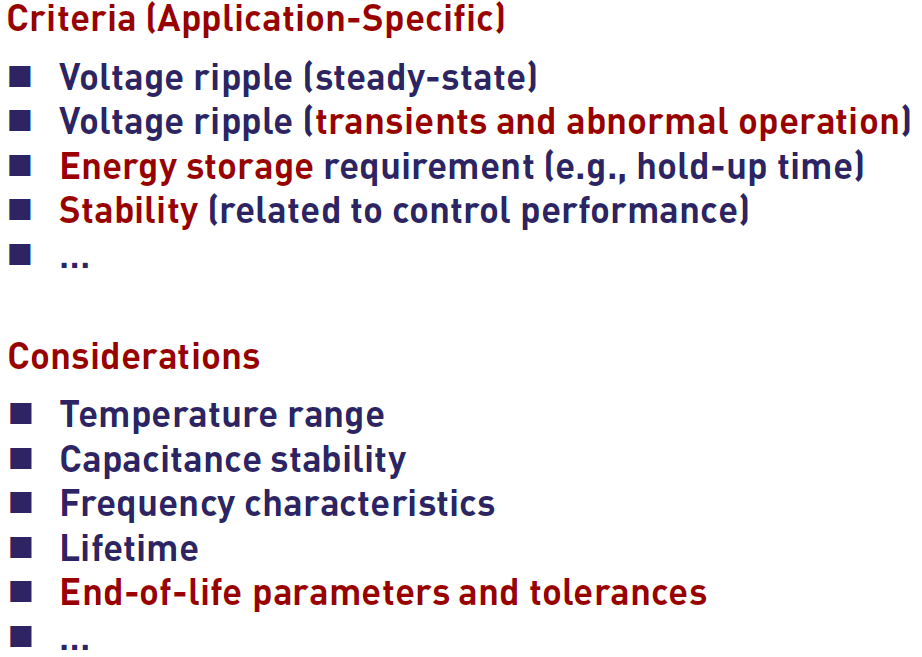
\includegraphics[width=\linewidth]{fig/lec08/DC_link_sizing_criteria.png}
        \caption{DC-link capacitor sizing criteria and practical considerations, Adapted from Huai Wang, \textit{Capacitors in Power Electronics Applications -- Reliability and Circuit Design}, IECON 2016 tutorial.}
    \end{figure}
\end{column}
\end{columns}
For high-reliability systems, the DC-link capacitor should be designed from the mission profile, not only from a single rated operating point.
\end{frame}


%%%%%%%%%%%%%%%%%%%%%%%%%%%%%%%%%%%%%%%%%%%%%%%%%%%%%%%%%%%%%
%% Ripple current and peak current
%%%%%%%%%%%%%%%%%%%%%%%%%%%%%%%%%%%%%%%%%%%%%%%%%%%%%%%%%%%%%
\begin{frame}
\frametitle{Step 3: RMS and Peak Current Rating}
The capacitor must withstand both RMS ripple current and peak current. The peak current caused by a voltage transition is
\begin{align}
    I_{\mathrm{pk}}
    =
    C\frac{dv}{dt}
\end{align}
The RMS current determines heating:
\begin{align}
    P_{\mathrm{ohmic}}
    =
    I_{\mathrm{rms}}^2 R_s
\end{align}
For a non-sinusoidal capacitor current composed of harmonics,
\begin{align}
    I_{\mathrm{rms}}
    =
    \sqrt{
    I_1^2+I_2^2+I_3^2+\cdots+I_n^2
    }
\end{align}
This is important because power-converter capacitor current is usually pulsed or nonsinusoidal.
\end{frame}

%%%%%%%%%%%%%%%%%%%%%%%%%%%%%%%%%%%%%%%%%%%%%%%%%%%%%%%%%%%%%
%% Losses and temperature rise
%%%%%%%%%%%%%%%%%%%%%%%%%%%%%%%%%%%%%%%%%%%%%%%%%%%%%%%%%%%%%
\begin{frame}
\frametitle{Step 4: Losses and Temperature Rise}
\begin{columns}
\begin{column}{0.56\textwidth}
After the voltage, capacitance and current ratings are selected, the thermal operating point must be checked. The total capacitor loss is
\begin{align}
    P_{\mathrm{loss}}
    =
    P_{\mathrm{ohmic}}
    +
    P_{\mathrm{dielectric}}
\end{align}
where
\begin{align}
    P_{\mathrm{ohmic}}
    =
    I_{\mathrm{rms}}^2R_s
\end{align}
and, for sinusoidal AC operation,
\begin{align}
    P_{\mathrm{dielectric}}
    =
    V_{\mathrm{pp}}^2\pi f_0 C \tan\delta_0
\end{align}
The temperature rise is
\begin{align}
    \Delta T
    =
    R_{\mathrm{th}}P_{\mathrm{loss}}
\end{align}
The design is acceptable only if the hot-spot temperature remains below the specified limit.
\end{column}
\begin{column}{0.40\textwidth}
    \vspace{-1cm}
\begin{figure}
    \centering
    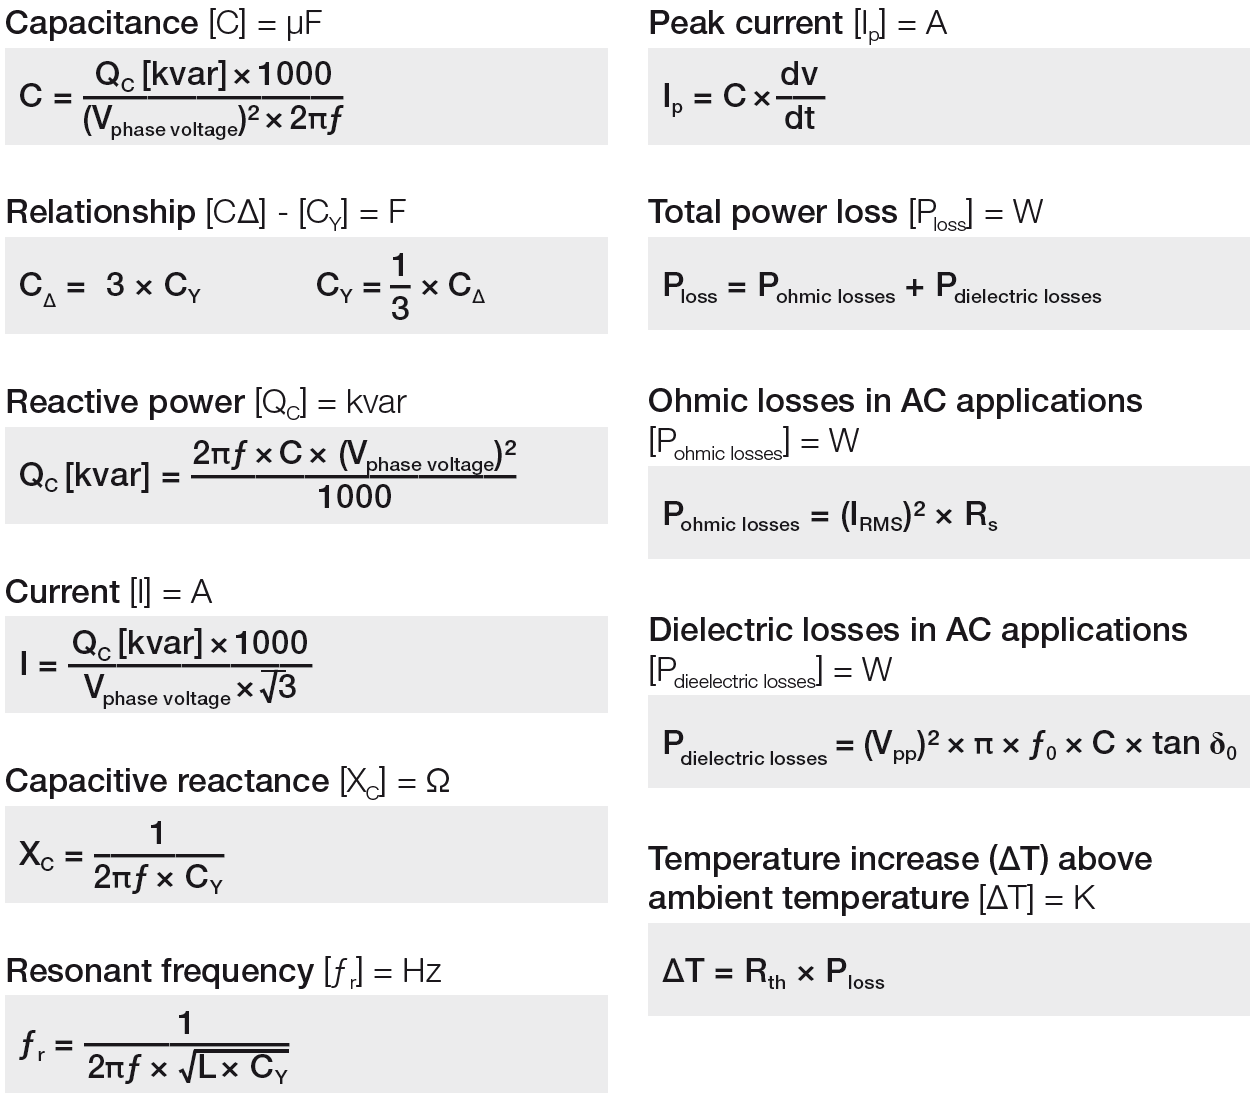
\includegraphics[width=\linewidth]{fig/lec08/losses_temperature_formulas.png}
    \caption{Useful power-electronics capacitor formulas for peak current, ohmic loss, dielectric loss and temperature rise. Adapted from FRAKO, \textit{Power Electronics Capacitors Selection Guide}}
\end{figure}
\end{column}
\end{columns}
\end{frame}


%%%%%%%%%%%%%%%%%%%%%%%%%%%%%%%%%%%%%%%%%%%%%%%%%%%%%%%%%%%%%
%% Series capacitor connection
%%%%%%%%%%%%%%%%%%%%%%%%%%%%%%%%%%%%%%%%%%%%%%%%%%%%%%%%%%%%%
\begin{frame}
\frametitle{Series Connection of Capacitors}

\begin{columns}
\begin{column}{0.56\textwidth}
Capacitors are connected in series when the required voltage rating exceeds the rating of one capacitor. For two capacitors in series,
\begin{align}
    C_{\mathrm{eq}}
    =
    \frac{C_1C_2}{C_1+C_2}
\end{align}
For identical capacitors, $C_{\mathrm{eq}}=\frac{C}{n}$, where \(n\) is the number of series-connected capacitors. The voltage sharing is affected by:
\begin{itemize}
    \item capacitance tolerance,
    \item leakage-current mismatch,
    \item insulation resistance mismatch,
    \item temperature variation and ageing.
\end{itemize}
Voltage-balancing resistors or active balancing circuits are therefore often required.
\end{column}

\begin{column}{0.40\textwidth}
    \vspace{-0.75cm}
\begin{figure}
    \centering
    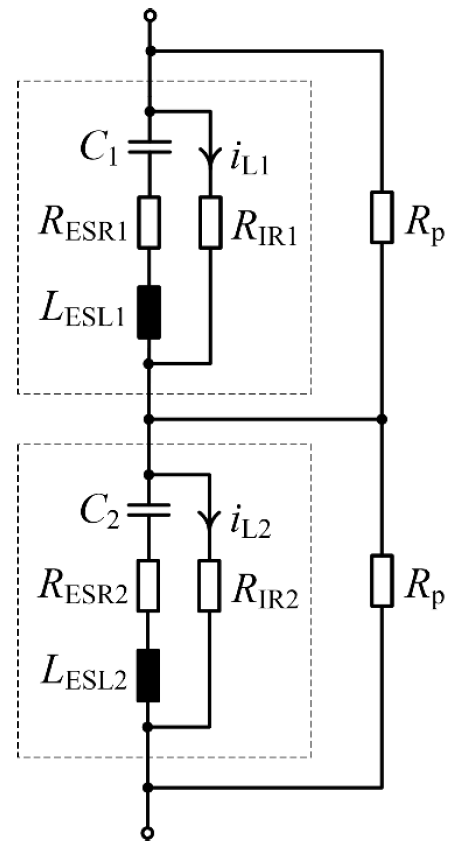
\includegraphics[width=0.4\linewidth]{fig/lec08/series_capacitor_balancing.png}
    \caption{Voltage balancing of series-connected capacitors with insulation resistance, leakage current and balancing resistance. Adapted from Huai Wang, \textit{Capacitors in Power Electronics Applications -- Reliability and Circuit Design}, IECON 2016 tutorial}
\end{figure}
\end{column}
\end{columns}
\end{frame}


%%%%%%%%%%%%%%%%%%%%%%%%%%%%%%%%%%%%%%%%%%%%%%%%%%%%%%%%%%%%%
%% Parallel capacitor connection
%%%%%%%%%%%%%%%%%%%%%%%%%%%%%%%%%%%%%%%%%%%%%%%%%%%%%%%%%%%%%
\begin{frame}
\frametitle{Parallel Connection of Capacitors}

\begin{columns}
\begin{column}{0.56\textwidth}
Capacitors are connected in parallel to increase capacitance, ripple-current capability, and reduce equivalent ESR. For capacitors connected in parallel,
\begin{align}
    C_{\mathrm{eq}}
    =
    C_1+C_2+C_3+\cdots
\end{align}
The equivalent ESR ideally becomes
\begin{align}
    ESR_{\mathrm{eq}}
    \approx
    \frac{ESR}{n}
\end{align}
for \(n\) identical capacitors. However, current sharing is not automatically equal. It depends on:
\begin{itemize}
    \item ESR and ESL mismatch,
    \item layout symmetry,
    \item terminal impedance,
    \item frequency.
\end{itemize}
\end{column}

\begin{column}{0.40\textwidth}
\begin{center}
\begin{circuitikz}[scale=0.82, transform shape]
    \draw (0,0) -- (4.2,0);
    \draw (0,-2.2) -- (4.2,-2.2);

    \draw (0.7,0) to[C,l=$C_1$] (0.7,-2.2);
    \draw (2.1,0) to[C,l=$C_2$] (2.1,-2.2);
    \draw (3.5,0) to[C,l=$C_3$] (3.5,-2.2);

    \draw[->, thick] (-0.5,-1.1) -- (0.2,-1.1);
    \node at (-0.85,-1.1) {$i_C$};

    \node at (2.1,-2.8) {\small parallel bank for higher current capability};
\end{circuitikz}
\end{center}
\begin{block}{Design Message}
\small
Parallel connection is effective only when the physical layout provides comparable impedance paths to all capacitors.
\end{block}
\end{column}
\end{columns}
A poor layout can cause one capacitor to carry excessive ripple current.
\end{frame}


%%%%%%%%%%%%%%%%%%%%%%%%%%%%%%%%%%%%%%%%%%%%%%%%%%%%%%%%%%%%%
%% Hybrid DC-link bank
%%%%%%%%%%%%%%%%%%%%%%%%%%%%%%%%%%%%%%%%%%%%%%%%%%%%%%%%%%%%%
\begin{frame}
\frametitle{Hybrid DC-Link Capacitor Bank}
\begin{columns}
\begin{column}{0.56\textwidth}
A hybrid DC-link bank combines capacitor technologies to exploit their complementary strengths. Typical arrangement:
\begin{itemize}
    \item electrolytic capacitors = large energy storage,
    \item film capacitors carry high ripple current and reduce mid-frequency impedance,
    \item ceramic or power ceramic capacitors suppress high-frequency switching transients.
\end{itemize}
This strategy improves:
\begin{itemize}
    \item ripple-current sharing and voltage ripple reduction,
    \item high-frequency decoupling and thermal distribution,
    \item lifetime of the electrolytic bank.
\end{itemize}
\end{column}

\begin{column}{0.40\textwidth}
    \vspace{-0.75cm}
\begin{figure}
    \centering
    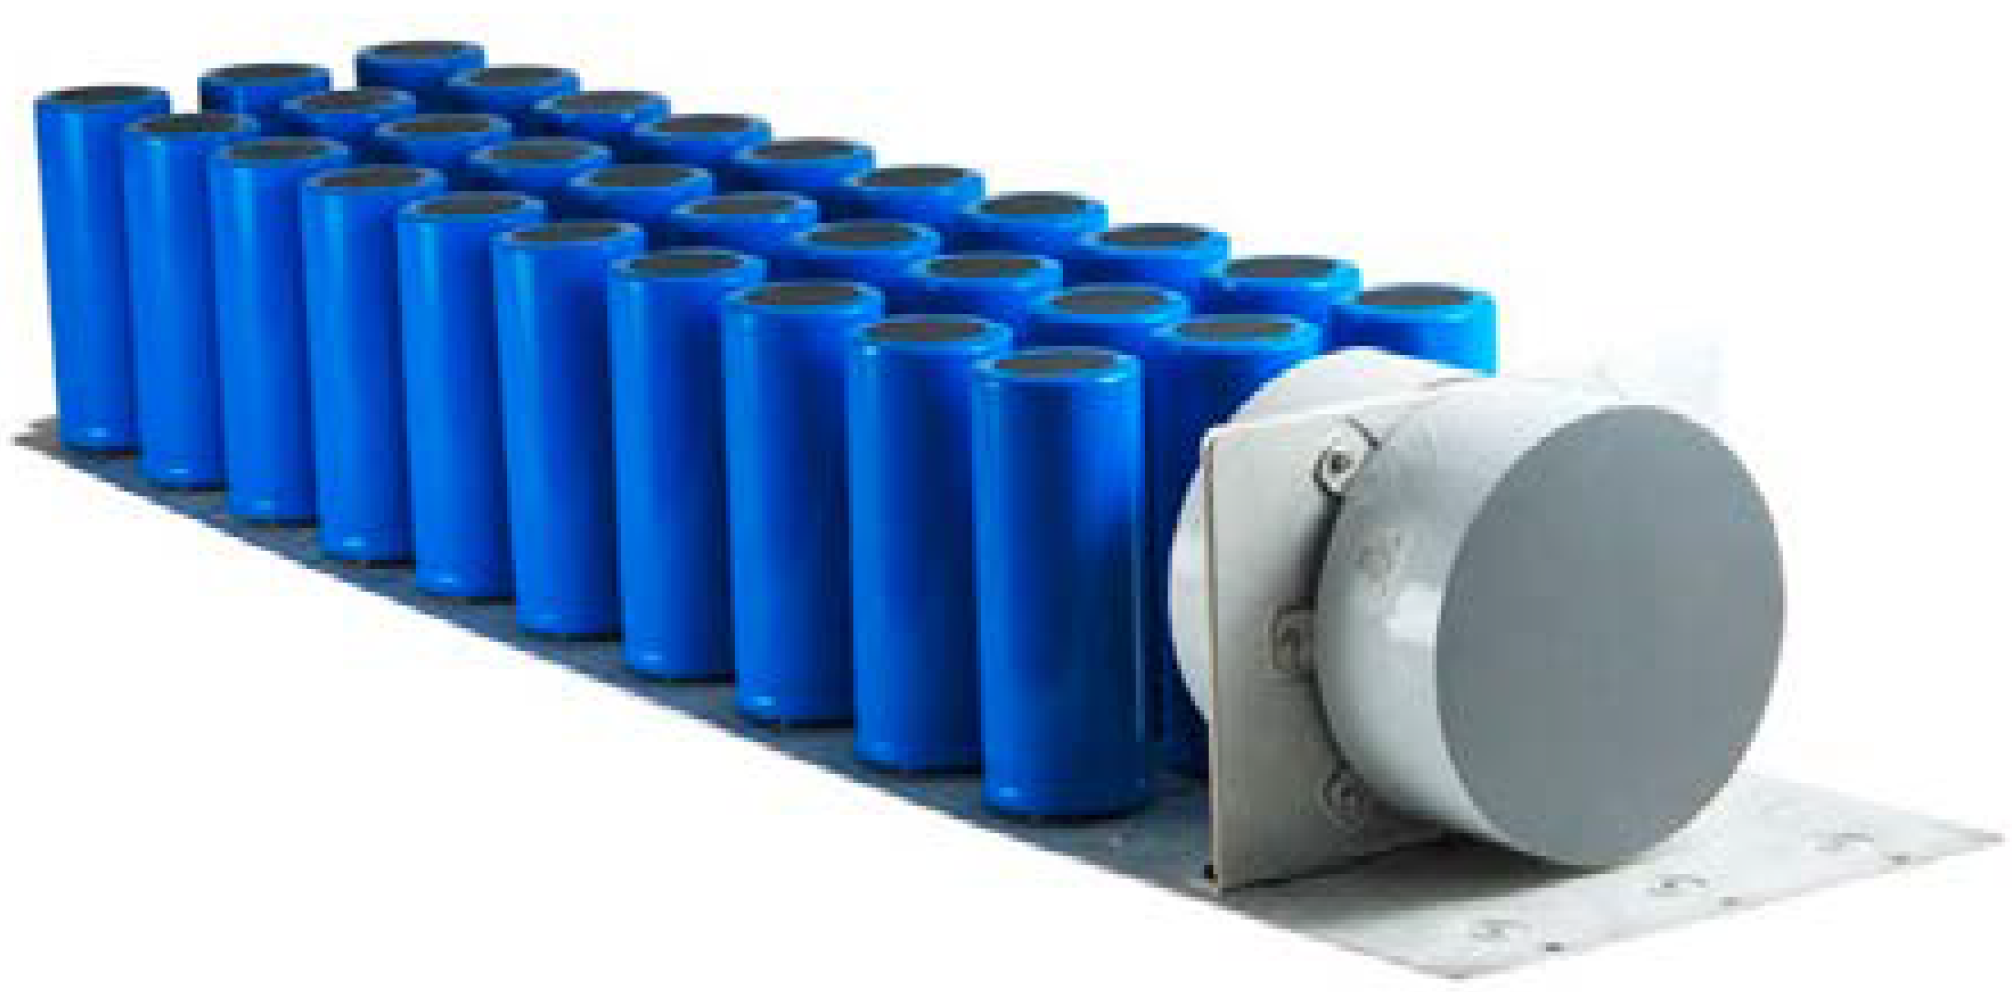
\includegraphics[width=\linewidth]{fig/lec08/hybrid_DC_link_bank.png}
    \caption{Hybrid DC-link capacitor bank showing ripple-current harmonic reduction by adding a film capacitor in parallel with an electrolytic bank. Adapted from Huai Wang, \textit{Capacitors in Power Electronics Applications -- Reliability and Circuit Design}, IECON 2016 tutorial}
\end{figure}
\end{column}
\end{columns}
The bank must still be checked for anti-resonance and layout-induced current imbalance.
\end{frame}


%%%%%%%%%%%%%%%%%%%%%%%%%%%%%%%%%%%%%%%%%%%%%%%%%%%%%%%%%%%%%
%% Low inductance DC link layout
%%%%%%%%%%%%%%%%%%%%%%%%%%%%%%%%%%%%%%%%%%%%%%%%%%%%%%%%%%%%%
\begin{frame}
\frametitle{Low-Inductance DC-Link Layout}
In fast-switching converters, the physical capacitor-bank layout can be as important as the capacitor datasheet. The DC-link loop inductance causes switching overvoltage:
\begin{align}
    v_{\sigma}
    =
    L_{\sigma}\frac{di}{dt}
\end{align}
Low-inductance design requires:
\begin{itemize}
    \item short current paths,
    \item laminated positive and negative busbars,
    \item magnetic-field cancellation,
    \item symmetric capacitor placement,
    \item local high-frequency capacitors near devices,
    \item minimized commutation-loop area.
\end{itemize}
For SiC and GaN converters, a low-ESL capacitor is insufficient if the busbar or PCB layout has large loop inductance.

\end{frame}

\begin{frame}
\frametitle{Low-Inductance DC-Link Layout}
\begin{figure}
    \centering
    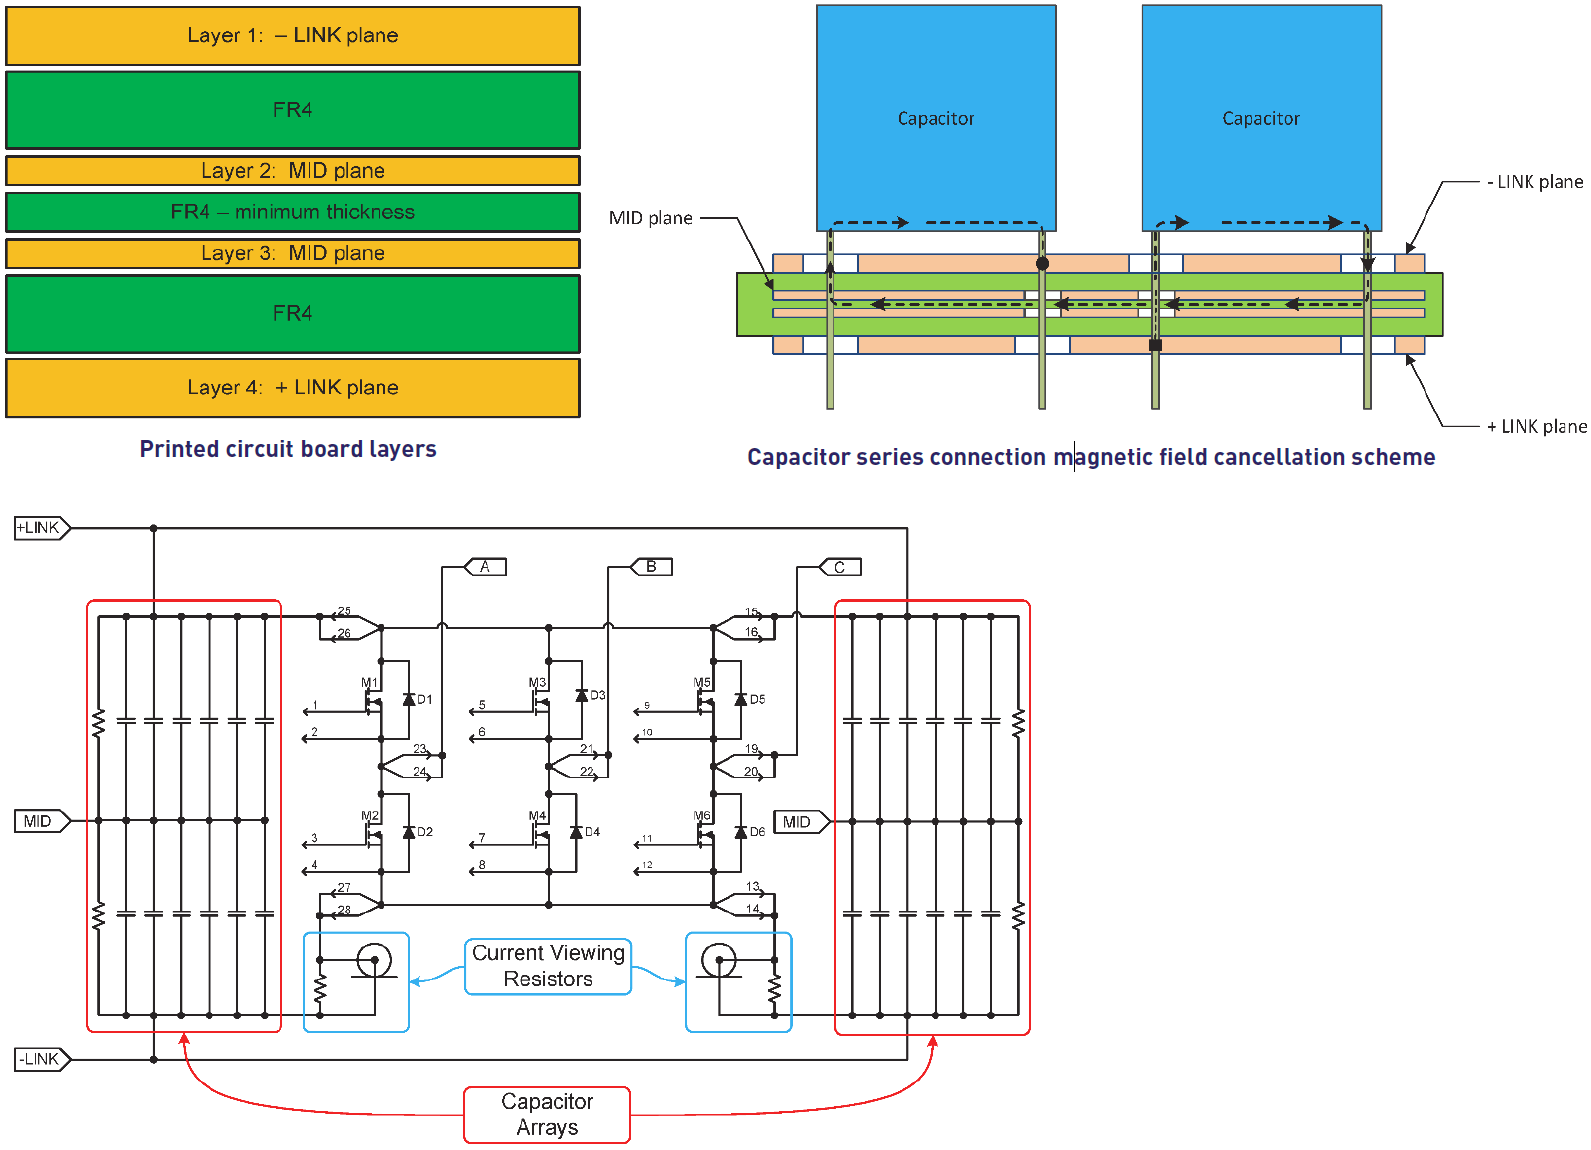
\includegraphics[width=0.5\linewidth]{fig/lec08/low_inductance_bank.png}
    \caption{Low-inductance capacitor-bank design using magnetic-field cancellation and PCB/busbar layout concepts. Adapted from Huai Wang, \textit{Capacitors in Power Electronics Applications -- Reliability and Circuit Design}, IECON 2016 tutorial}
\end{figure}
\end{frame}

%%%%%%%%%%%%%%%%%%%%%%%%%%%%%%%%%%%%%%%%%%%%%%%%%%%%%%%%%%%%%
%% Selection verification checklist
%%%%%%%%%%%%%%%%%%%%%%%%%%%%%%%%%%%%%%%%%%%%%%%%%%%%%%%%%%%%%
\begin{frame}
\frametitle{Final Capacitor Selection Checklist}

\begin{itemize}
    \item \textbf{Voltage check:}
    \[
        V_{\mathrm{rated}} > V_{\mathrm{max,operating}} + V_{\mathrm{surge\ margin}}
    \]

    \item \textbf{Capacitance check:}
    \[
        C_{\mathrm{effective}} \geq C_{\mathrm{required}}
    \]
    using bias, temperature, tolerance and ageing corrections.

    \item \textbf{Ripple-current check:} $I_{\mathrm{C,rms}} < I_{\mathrm{rated,rms}}$.

    \item \textbf{Peak-current and \(dv/dt\) check:}
    \[
        I_{\mathrm{pk}} = C\frac{dv}{dt}
    \]

    \item \textbf{Thermal check:}
    \[
        T_{\mathrm{hotspot}} = T_{\mathrm{amb}} + R_{\mathrm{th}}P_{\mathrm{loss}}
    \]
    \item \textbf{Impedance check:}
    ESR, ESL, self-resonance, anti-resonance and layout parasitics must satisfy the required frequency-domain impedance.
    \item \textbf{Reliability check:}
    lifetime, end-of-life capacitance loss, ESR increase, leakage current and mission-profile stress must be acceptable.
\end{itemize}
\end{frame}


%%%%%%%%%%%%%%%%%%%%%%%%%%%%%%%%%%%%%%%%%%%%%%%%%%%%%%%%%%%%%
%% Losses, thermal design, reliability
%%%%%%%%%%%%%%%%%%%%%%%%%%%%%%%%%%%%%%%%%%%%%%%%%%%%%%%%%%%%%
\begin{frame}
\begin{center}
  \textbf{\Huge{Losses, Thermal Design, and Reliability}}\\[0.4cm]
  \textbf{\Large{From Electrical Stress to Lifetime and Condition Monitoring}}
\end{center}
\end{frame}


%%%%%%%%%%%%%%%%%%%%%%%%%%%%%%%%%%%%%%%%%%%%%%%%%%%%%%%%%%%%%
%% Loss mechanisms in capacitors
%%%%%%%%%%%%%%%%%%%%%%%%%%%%%%%%%%%%%%%%%%%%%%%%%%%%%%%%%%%%%
\begin{frame}
\frametitle{Loss Mechanisms in Capacitors}

\begin{columns}
\begin{column}{0.56\textwidth}
Real capacitors dissipate power due to ripple current, AC voltage, leakage, and switching transients. Main loss mechanisms:
\begin{itemize}
    \item \textbf{Ohmic loss:} caused by ESR under RMS ripple current.
    \item \textbf{Dielectric loss:} caused by polarization loss in the dielectric.
    \item \textbf{Leakage loss:} caused by finite insulation resistance.
    \item \textbf{Terminal and contact loss:} caused by current flowing through tabs, terminals, busbars, and solder joints.
    \item \textbf{Layout-related loss:} caused by high-frequency current crowding and parasitic inductance.
\end{itemize}
\end{column}

\begin{column}{0.44\textwidth}
\begin{center}
\begin{circuitikz}[scale=0.78, transform shape]
    \tikzstyle{block} = [draw, rounded corners, align=center,
    minimum width=2.4cm, minimum height=0.62cm, font=\scriptsize]

    \node[block, minimum width=3.0cm] (total) at (0,0) {Total capacitor\\loss};

    \node[block] (esr) at (-3.2,-1.5) {ESR\\loss};
    \node[block] (diel) at (0,-1.5) {Dielectric\\loss};
    \node[block] (leak) at (3.2,-1.5) {Leakage\\loss};

    \node[block] (ripple) at (-3.2,-3.0) {Ripple current\\$I_{\mathrm{rms}}$};
    \node[block] (tan) at (0,-3.0) {$\tan\delta$ and\\AC voltage};
    \node[block] (dc) at (3.2,-3.0) {DC voltage and\\insulation};

    \draw[->, thick] (total) -- (esr);
    \draw[->, thick] (total) -- (diel);
    \draw[->, thick] (total) -- (leak);

    \draw[->, thick] (esr) -- (ripple);
    \draw[->, thick] (diel) -- (tan);
    \draw[->, thick] (leak) -- (dc);
\end{circuitikz}
\end{center}

\end{column}
\end{columns}

\end{frame}


%%%%%%%%%%%%%%%%%%%%%%%%%%%%%%%%%%%%%%%%%%%%%%%%%%%%%%%%%%%%%
%% Loss mechanisms in capacitors
%%%%%%%%%%%%%%%%%%%%%%%%%%%%%%%%%%%%%%%%%%%%%%%%%%%%%%%%%%%%%
\begin{frame}
\frametitle{Loss Mechanisms in Capacitors}

\begin{columns}
\begin{column}{0.56\textwidth}
The first-order power loss is usually estimated as
\begin{align}
    P_{\mathrm{loss}}
    =
    I_{\mathrm{rms}}^2R_{\mathrm{ESR}}
    +
    P_{\mathrm{dielectric}}
    +
    P_{\mathrm{leak}}
\end{align}
\end{column}

\begin{column}{0.40\textwidth}
\begin{block}{Message}
\small
Capacitor loss is not only an efficiency issue. It directly determines hot-spot temperature, ageing speed, capacitance drift, ESR increase, and ultimately lifetime.
\end{block}
\end{column}
\end{columns}

\end{frame}

%%%%%%%%%%%%%%%%%%%%%%%%%%%%%%%%%%%%%%%%%%%%%%%%%%%%%%%%%%%%%
%% Thermal model
%%%%%%%%%%%%%%%%%%%%%%%%%%%%%%%%%%%%%%%%%%%%%%%%%%%%%%%%%%%%%
\begin{frame}
\frametitle{Thermal Model of a Capacitor}
\begin{columns}
\begin{column}{0.56\textwidth}
The losses generated inside the capacitor increase the internal hot-spot temperature. A first-order thermal model is
\begin{align}
    T_{\mathrm{hotspot}}
    =
    T_{\mathrm{amb}}
    +
    R_{\mathrm{th}}P_{\mathrm{loss}}
\end{align}
where
\begin{itemize}
    \item \(T_{\mathrm{hotspot}}\) is the internal hot-spot temperature,
    \item \(T_{\mathrm{amb}}\) is ambient temperature,
    \item \(R_{\mathrm{th}}\) is the thermal resistance from hot spot to ambient,
    \item \(P_{\mathrm{loss}}\) is total capacitor power loss.
\end{itemize}
The design must satisfy
\begin{align}
    T_{\mathrm{hotspot}} < T_{\mathrm{max}}
\end{align}
under worst-case ambient temperature, ripple current, cooling condition, and ageing state.
\end{column}

\begin{column}{0.40\textwidth}
\begin{center}
\begin{circuitikz}[scale=0.82, transform shape]
    \draw (0,0) to[I,l=$P_{\mathrm{loss}}$] (0,2.0);
    \draw (0,2.0) -- (1.6,2.0);
    \draw (1.6,2.0) to[R,l=$R_{\mathrm{th}}$] (1.6,0);
    \draw (1.6,0) -- (0,0);

    \node at (2.45,2.0) {$T_{\mathrm{hotspot}}$};
    \node at (2.25,0) {$T_{\mathrm{amb}}$};
    \node at (0.7,-0.45) {\small thermal equivalent circuit};
\end{circuitikz}
\end{center}

\begin{block}{Practical Note}
\small
For large-can electrolytic capacitors with significant ripple current, the internal core temperature can be noticeably higher than the case temperature. This must be considered during lifetime estimation.
\end{block}
\end{column}
\end{columns}

\end{frame}


%%%%%%%%%%%%%%%%%%%%%%%%%%%%%%%%%%%%%%%%%%%%%%%%%%%%%%%%%%%%%
%% Electrolytic capacitor lifetime
%%%%%%%%%%%%%%%%%%%%%%%%%%%%%%%%%%%%%%%%%%%%%%%%%%%%%%%%%%%%%
\begin{frame}
\frametitle{Aluminum Electrolytic Capacitor Lifetime}
\begin{columns}
\begin{column}{0.5\textwidth}
Aluminum electrolytic capacitors are often lifetime-critical because their electrolyte gradually evaporates or degrades during operation. The usual ageing effects are:
\begin{itemize}
    \item capacitance decreases,
    \item ESR increases,
    \item leakage current may change,
    \item internal temperature rises further due to higher ESR,
    \item open-circuit wear-out becomes likely.
\end{itemize}
\end{column}

\begin{column}{0.5\textwidth}
A commonly used lifetime expression is
\begin{align}
    L_{\mathrm{op}}
    =
    M_v L_b
    2^{(T_m-T_a)/10}
\end{align}
\begin{itemize}
    \item \(L_{\mathrm{op}}\) is expected operating life,
    \item \(L_b\) is base life,
    \item \(T_m\) is maximum permitted internal temperature,
    \item \(T_a\) is actual internal operating temperature,
    \item \(M_v\) accounts for voltage derating.
\end{itemize}
\end{column}
\end{columns}
\begin{block}{Rule of Thumb}
\small
For many aluminum electrolytic capacitors, operating life approximately doubles for every \(10^\circ\mathrm{C}\) reduction in internal temperature.
\end{block}
\end{frame}


%%%%%%%%%%%%%%%%%%%%%%%%%%%%%%%%%%%%%%%%%%%%%%%%%%%%%%%%%%%%%
%% Load life and end of life
%%%%%%%%%%%%%%%%%%%%%%%%%%%%%%%%%%%%%%%%%%%%%%%%%%%%%%%%%%%%%
\begin{frame}
\frametitle{Load Life Test and End-of-Life Criteria}
\begin{columns}
\begin{column}{0.56\textwidth}
Capacitor lifetime is usually specified under a rated load-life test condition. For aluminum electrolytic capacitors, the test commonly applies:
\begin{itemize}
    \item rated temperature,
    \item DC voltage,
    \item AC ripple current,
    \item specified test duration,
    \item post-test stabilization before measurement.
\end{itemize}
\end{column}

\begin{column}{0.40\textwidth}
\begin{block}{Design Message}
\small
The capacitor that satisfies capacitance and voltage on day one may still be unacceptable if its end-of-life capacitance, ESR, or leakage current violates converter requirements.
\end{block}
\end{column}
\end{columns}

\end{frame}


%%%%%%%%%%%%%%%%%%%%%%%%%%%%%%%%%%%%%%%%%%%%%%%%%%%%%%%%%%%%%
%% Load life and end of life
%%%%%%%%%%%%%%%%%%%%%%%%%%%%%%%%%%%%%%%%%%%%%%%%%%%%%%%%%%%%%
\begin{frame}
\frametitle{Load Life Test and End-of-Life Criteria}
\begin{columns}
\begin{column}{0.56\textwidth}
Typical end-of-life indicators include:
\begin{itemize}
    \item capacitance below an allowed fraction of initial value,
    \item ESR above an allowed limit,
    \item leakage current above specification,
    \item mechanical damage,
    \item electrolyte leakage,
    \item open-circuit or short-circuit failure.
\end{itemize}
\end{column}

\begin{column}{0.40\textwidth}
\begin{block}{Design Message}
\small
The capacitor that satisfies capacitance and voltage on day one may still be unacceptable if its end-of-life capacitance, ESR, or leakage current violates converter requirements.
\end{block}
\end{column}
\end{columns}
In converter design, lifetime should be evaluated at the actual hot-spot temperature and ripple-current condition, not only at datasheet nominal conditions.
\end{frame}

%%%%%%%%%%%%%%%%%%%%%%%%%%%%%%%%%%%%%%%%%%%%%%%%%%%%%%%%%%%%%
%% Load-life and ripple-life test
%%%%%%%%%%%%%%%%%%%%%%%%%%%%%%%%%%%%%%%%%%%%%%%%%%%%%%%%%%%%%
\begin{frame}
\frametitle{Load-Life and Ripple-Life Test of Capacitors}

\begin{columns}
\begin{column}{0.52\textwidth}
\textbf{Load-life test}
\begin{itemize}
    \item Capacitors are placed in a circulating-air oven at the upper rated temperature: $85^\circ\mathrm{C},\;105^\circ\mathrm{C},\;125^\circ\mathrm{C}$.
    \item A DC voltage and AC ripple voltage are applied simultaneously.
    \item The AC voltage is adjusted so that the rated ripple current flows.
    \item The DC voltage is adjusted so that the capacitor peak voltage equals the rated voltage.
    \item After the rated test duration, capacitors are stabilized at \(25^\circ\mathrm{C}\) for at least 24 h before measurement.
\end{itemize}
\end{column}

\begin{column}{0.48\textwidth}
\textbf{EIA ripple-life test}
\begin{itemize}
    \item Ripple current is usually applied at \(120~\si{\hertz}\).
    \item Test temperature is typically: $85 \pm 2^\circ\mathrm{C}$.
    \item Airflow is kept low to avoid excessive cooling.
    \item Samples are periodically measured during the test.
\end{itemize}
\begin{block}{End-of-Life Criteria}
\small
A capacitor reaches end of life if: 

$C < 80\%\,C_0 \quad \text{or}  \quad ESR > 200\%\,ESR_0  \quad \text{or}  \quad DCL > DCL_0$ or mechanical damage / electrolyte leakage is observed.
\end{block}
\end{column}
\end{columns}


\end{frame}

%%%%%%%%%%%%%%%%%%%%%%%%%%%%%%%%%%%%%%%%%%%%%%%%%%%%%%%%%%%%%
%% Failure modes aluminium electrolytic
%%%%%%%%%%%%%%%%%%%%%%%%%%%%%%%%%%%%%%%%%%%%%%%%%%%%%%%%%%%%%
\begin{frame}
\frametitle{Failure Modes of Aluminum Electrolytic Capacitors}
\begin{columns}
\begin{column}{0.56\textwidth}
Aluminum electrolytic capacitors can fail by early-life, random, or wear-out mechanisms.Important failure modes include:

\begin{itemize}
    \item \textbf{Open circuit:}
    \begin{itemize}
        \item electrolyte loss,
        \item terminal connection failure,
        \item internal pressure or venting.
    \end{itemize}

    \item \textbf{Short circuit:}
    \begin{itemize}
        \item oxide dielectric breakdown,
        \item severe overvoltage or thermal stress.
    \end{itemize}

    \item \textbf{Wear-out drift:}
    \begin{itemize}
        \item capacitance reduction,
        \item ESR and $\tan\delta$ increase
        \item leakage-current variation.
    \end{itemize}
\end{itemize}
\end{column}

\begin{column}{0.40\textwidth}
    \vspace{-0.5cm}
\begin{figure}
    \centering
    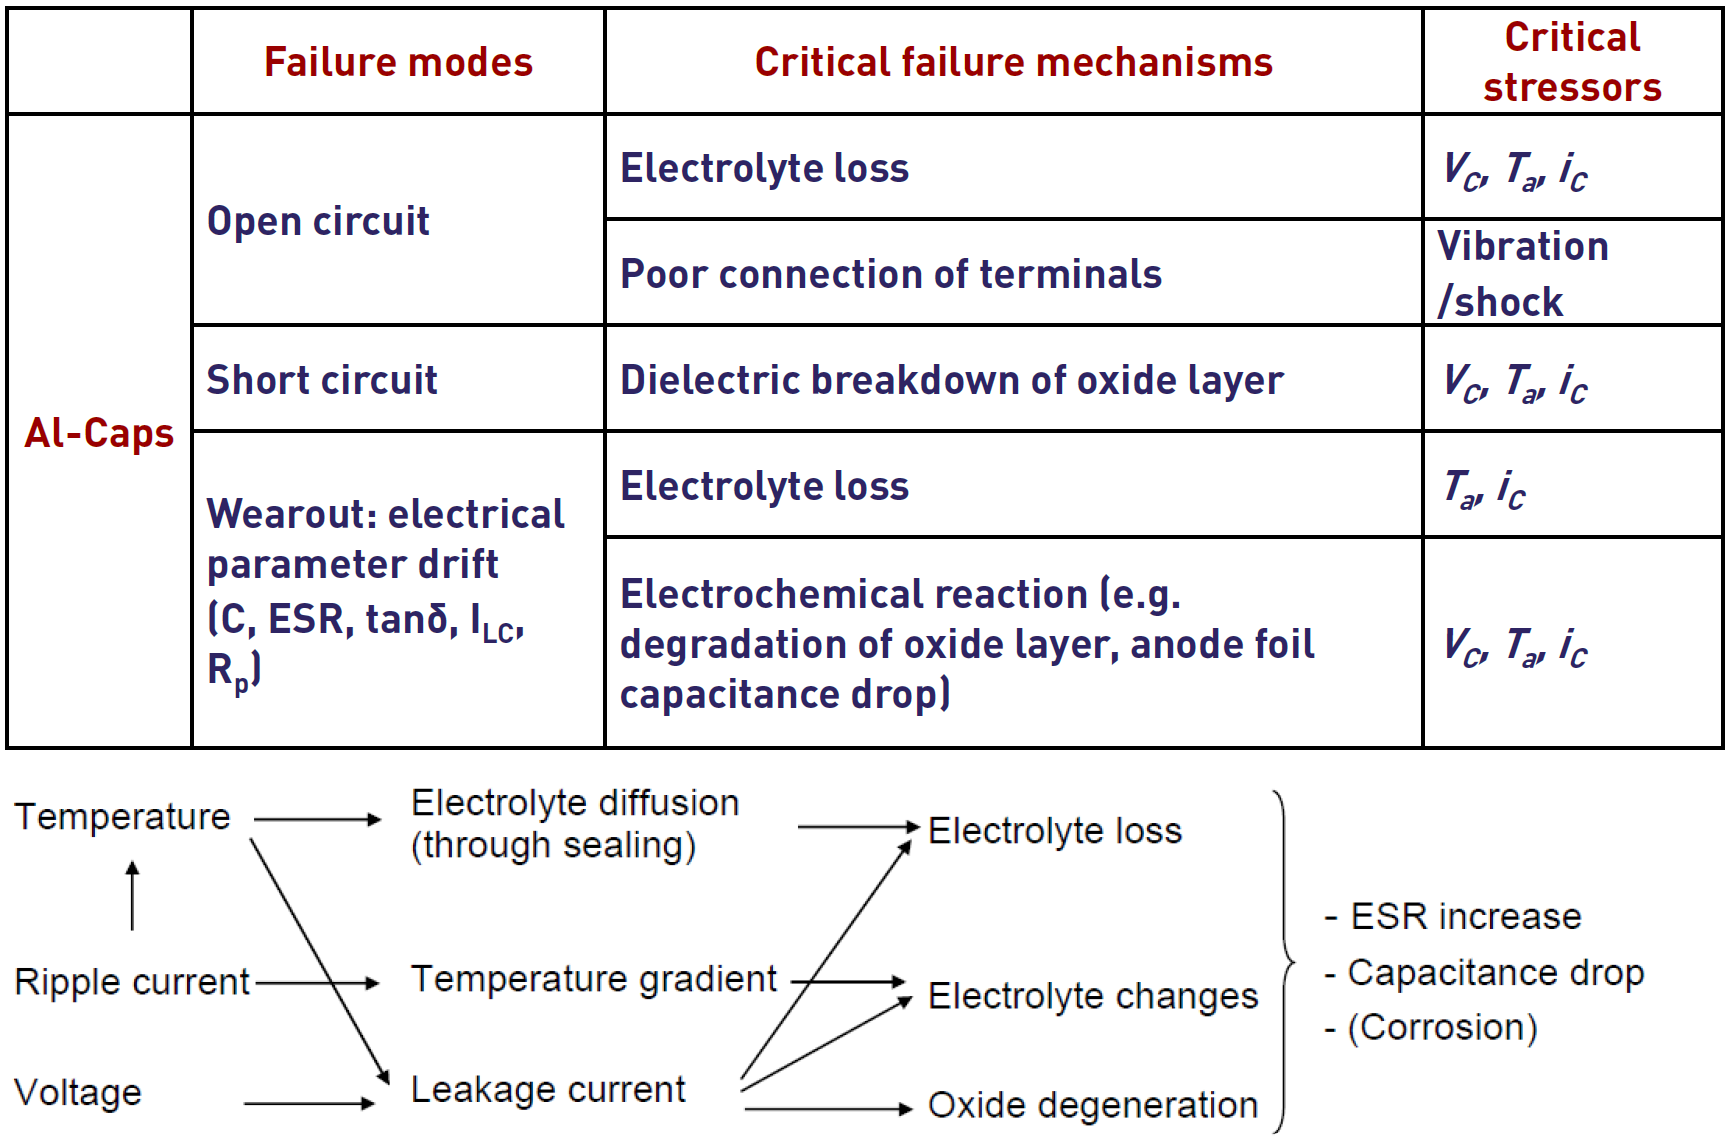
\includegraphics[width=\linewidth]{fig/lec08/AlCap_failure_modes.png}
    \caption{Failure modes, mechanisms, and critical stressors of aluminum electrolytic capacitors. Adapted from Huai Wang, \textit{Capacitors in Power Electronics Applications -- Reliability and Circuit Design}, IECON 2016 tutorial}
\end{figure}
\end{column}
\end{columns}
Critical stressors are voltage \(V_C\), ambient or hot-spot temperature \(T_a\), capacitor ripple current \(i_C\), and mechanical vibration or shock.
\end{frame}


%%%%%%%%%%%%%%%%%%%%%%%%%%%%%%%%%%%%%%%%%%%%%%%%%%%%%%%%%%%%%
%% Failure modes film capacitors
%%%%%%%%%%%%%%%%%%%%%%%%%%%%%%%%%%%%%%%%%%%%%%%%%%%%%%%%%%%%%
\begin{frame}
\frametitle{Failure Modes of Metallized Film Capacitors}
\begin{columns}
\begin{column}{0.56\textwidth}
Metallized polypropylene film capacitors are used in DC links, AC filters, and snubbers for low loss and self-healing. Main failure mechanisms are:
\begin{itemize}
    \item metallization corrosion due to humidity,
    \item capacitance loss from reduced active area,
    \item self-healing events under overvoltage or overcurrent,
    \item dielectric breakdown under high voltage or \(dv/dt\),
    \item connection instability from thermal and mechanical stress.
\end{itemize}
End-of-life usually shows gradual capacitance loss rather than sudden short circuit. Severe overvoltage, partial discharge, or thermal overload can still cause destructive failure.
\end{column}

\begin{column}{0.40\textwidth}
\begin{figure}
    \centering
    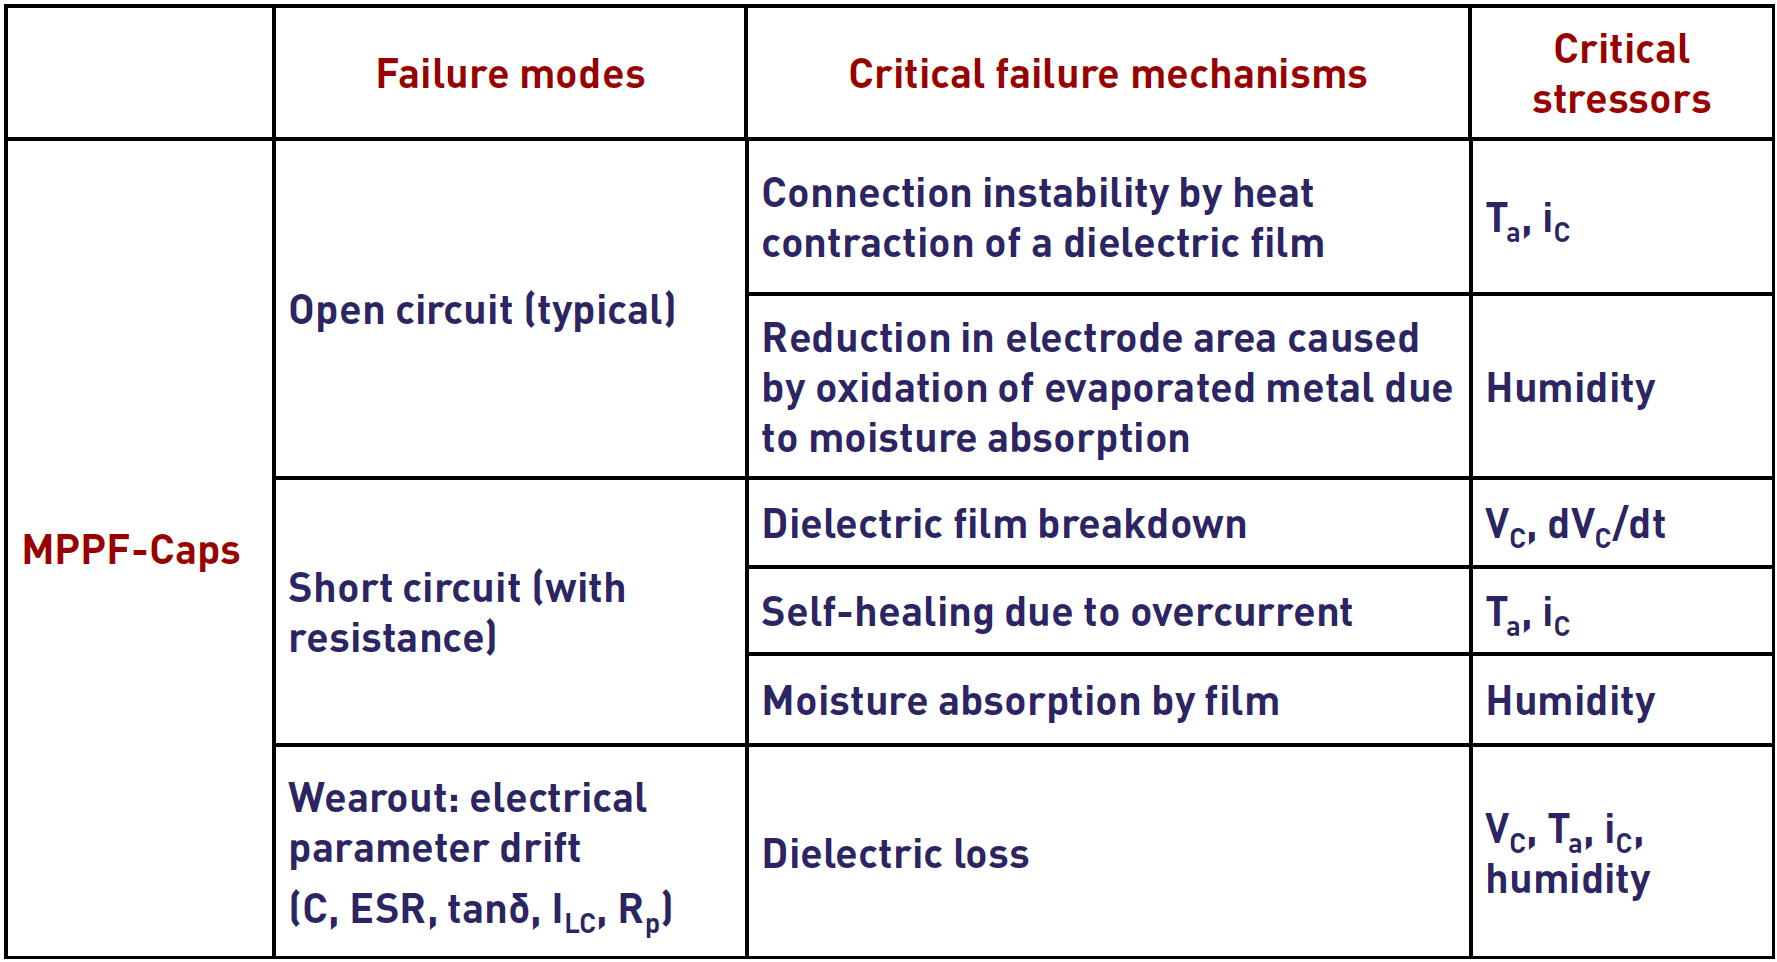
\includegraphics[width=\linewidth]{fig/lec08/MPPF_failure_modes.png}
    \caption{Failure modes, mechanisms, and critical stressors of metallized polypropylene film capacitors. Adapted from Huai Wang, \textit{Capacitors in Power Electronics Applications -- Reliability and Circuit Design}, IECON 2016 tutorial}
\end{figure}
\end{column}
\end{columns}

\end{frame}


%%%%%%%%%%%%%%%%%%%%%%%%%%%%%%%%%%%%%%%%%%%%%%%%%%%%%%%%%%%%%
%% Failure modes MLCC
%%%%%%%%%%%%%%%%%%%%%%%%%%%%%%%%%%%%%%%%%%%%%%%%%%%%%%%%%%%%%
\begin{frame}
\frametitle{Failure Modes of Multilayer Ceramic Capacitors}
\begin{columns}
\begin{column}{0.56\textwidth}
MLCCs offer excellent high-frequency performance, but fail differently from electrolytic and film capacitors. Key stress mechanisms include:

\begin{itemize}
    \item dielectric breakdown under voltage, temperature, and current stress,
    \item flex cracking from PCB bending,
    \item thermal shock cracking,
    \item mechanical damage during assembly,
    \item insulation degradation,
    \item micro-crack growth in the ceramic body.
\end{itemize}
A cracked MLCC may fail short circuit, which is critical in DC-link applications. MLCCs require careful PCB placement, soldering profile, board flex control, and voltage derating.

\end{column}

\begin{column}{0.40\textwidth}
\begin{figure}
    \centering
    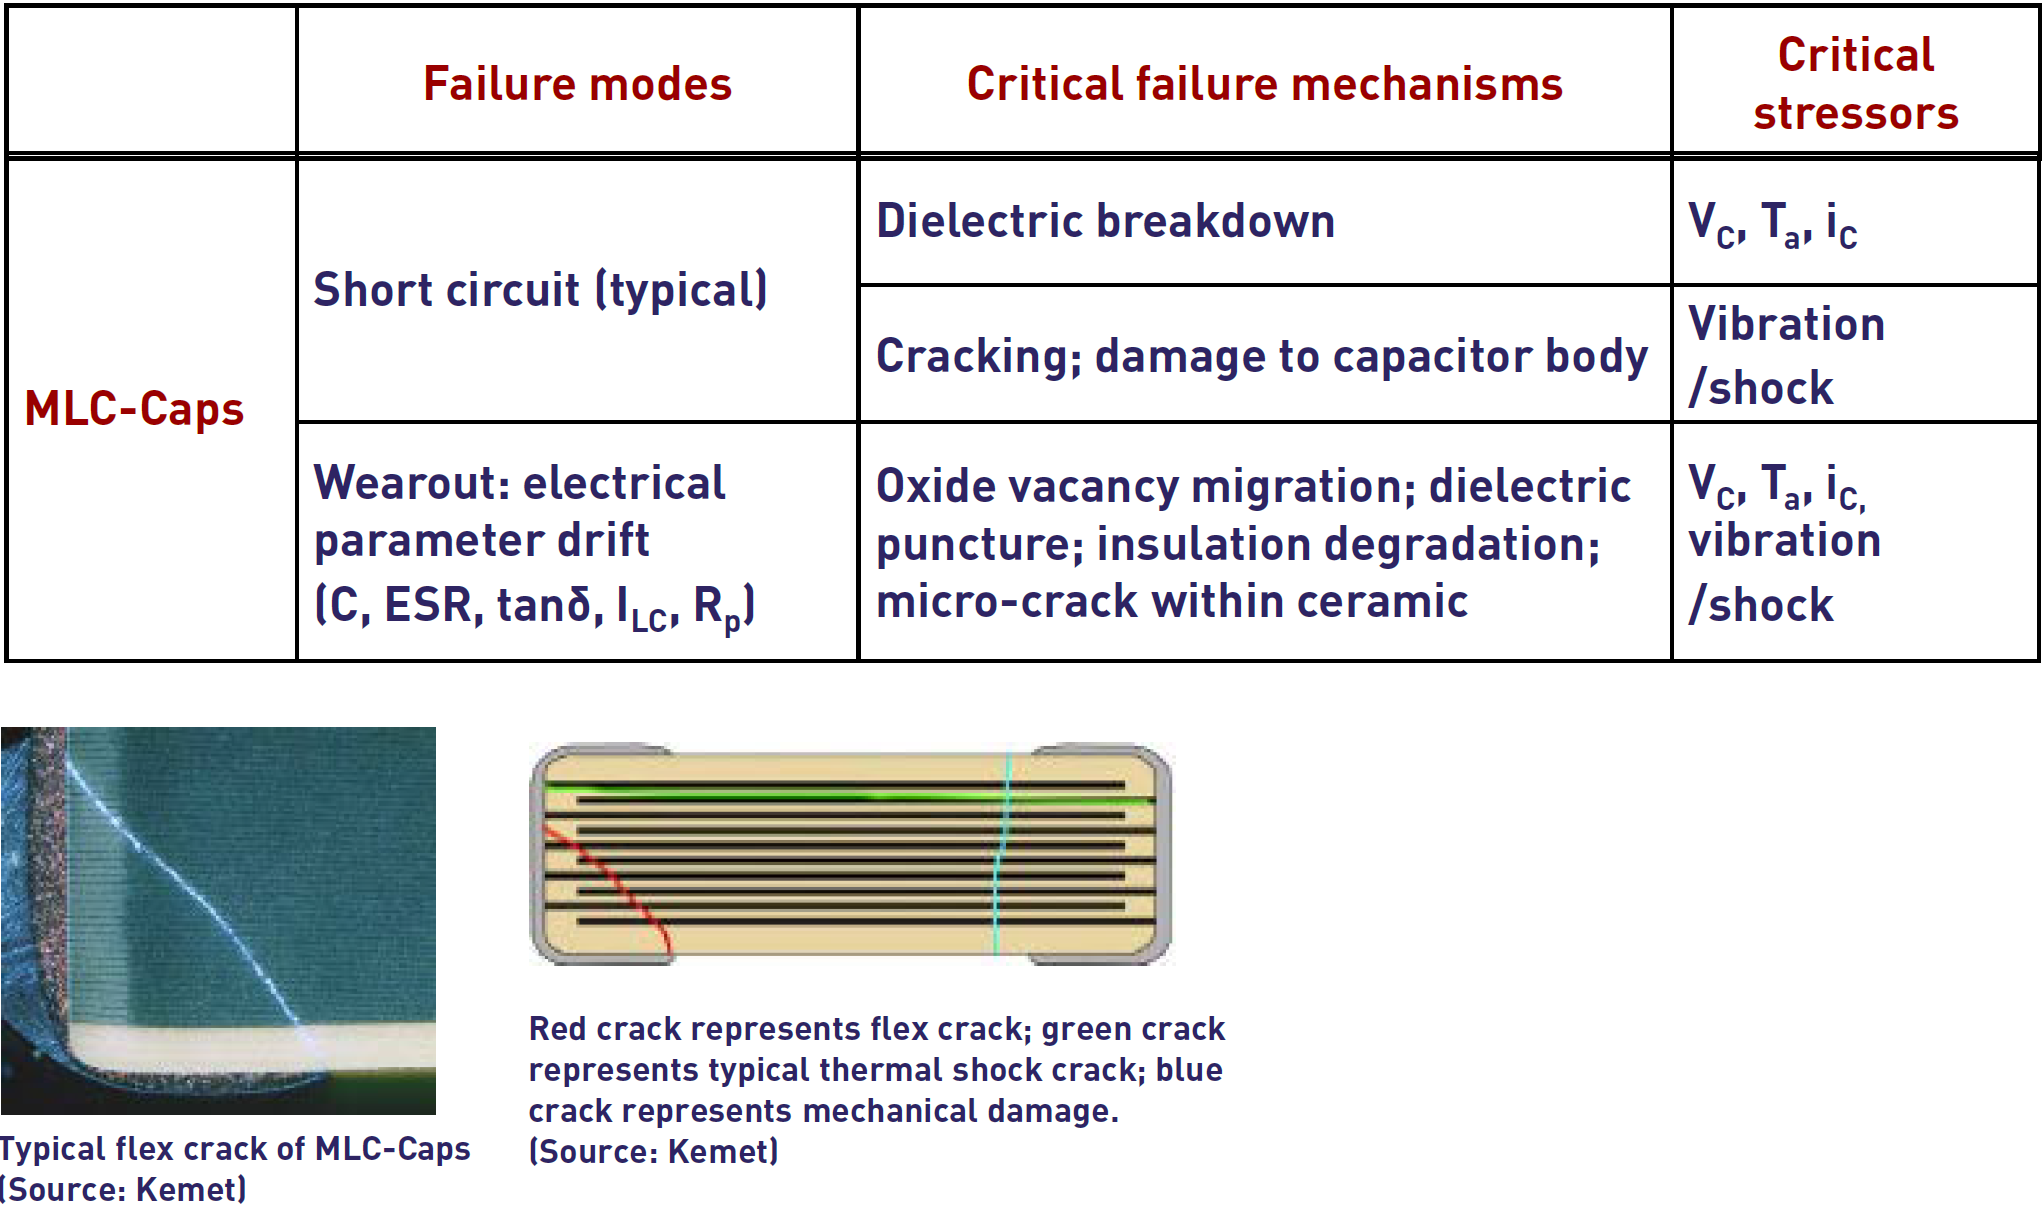
\includegraphics[width=\linewidth]{fig/lec08/MLCC_failure_modes.png}
    \caption{Failure modes, mechanisms, and critical stressors of multilayer ceramic capacitors, including flex and thermal-shock cracking. Adapted from Huai Wang, \textit{Capacitors in Power Electronics Applications -- Reliability and Circuit Design}, IECON 2016 tutorial}
\end{figure}
\end{column}
\end{columns}
\end{frame}


%%%%%%%%%%%%%%%%%%%%%%%%%%%%%%%%%%%%%%%%%%%%%%%%%%%%%%%%%%%%%
%% Failure mode comparison
%%%%%%%%%%%%%%%%%%%%%%%%%%%%%%%%%%%%%%%%%%%%%%%%%%%%%%%%%%%%%
\begin{frame}
\frametitle{Comparison of Failure Behaviour}

\begin{columns}
\begin{column}{0.6\textwidth}
Capacitors age and fail differently.
\begin{itemize}
    \item \textbf{Aluminum electrolytic capacitors}
    \begin{itemize}
        \item dominant failure mode: wear-out,
        \item typical failure: open circuit or parameter drift,
        \item critical stressors: temperature, voltage, ripple current.
    \end{itemize}

    \item \textbf{Metallized film capacitors}
    \begin{itemize}
        \item dominant failure mode: open circuit or capacitance loss,
        \item self-healing capability is good,
        \item critical stressors: humidity, voltage, temperature, ripple current.
    \end{itemize}

    \item \textbf{MLCCs}
    \begin{itemize}
        \item dominant failure mode: short circuit,
        \item no self-healing capability,
        \item critical stressors: voltage, temperature, vibration, shock and board flex.
    \end{itemize}
\end{itemize}

\end{column}

\begin{column}{0.40\textwidth}
\begin{figure}
    \centering
    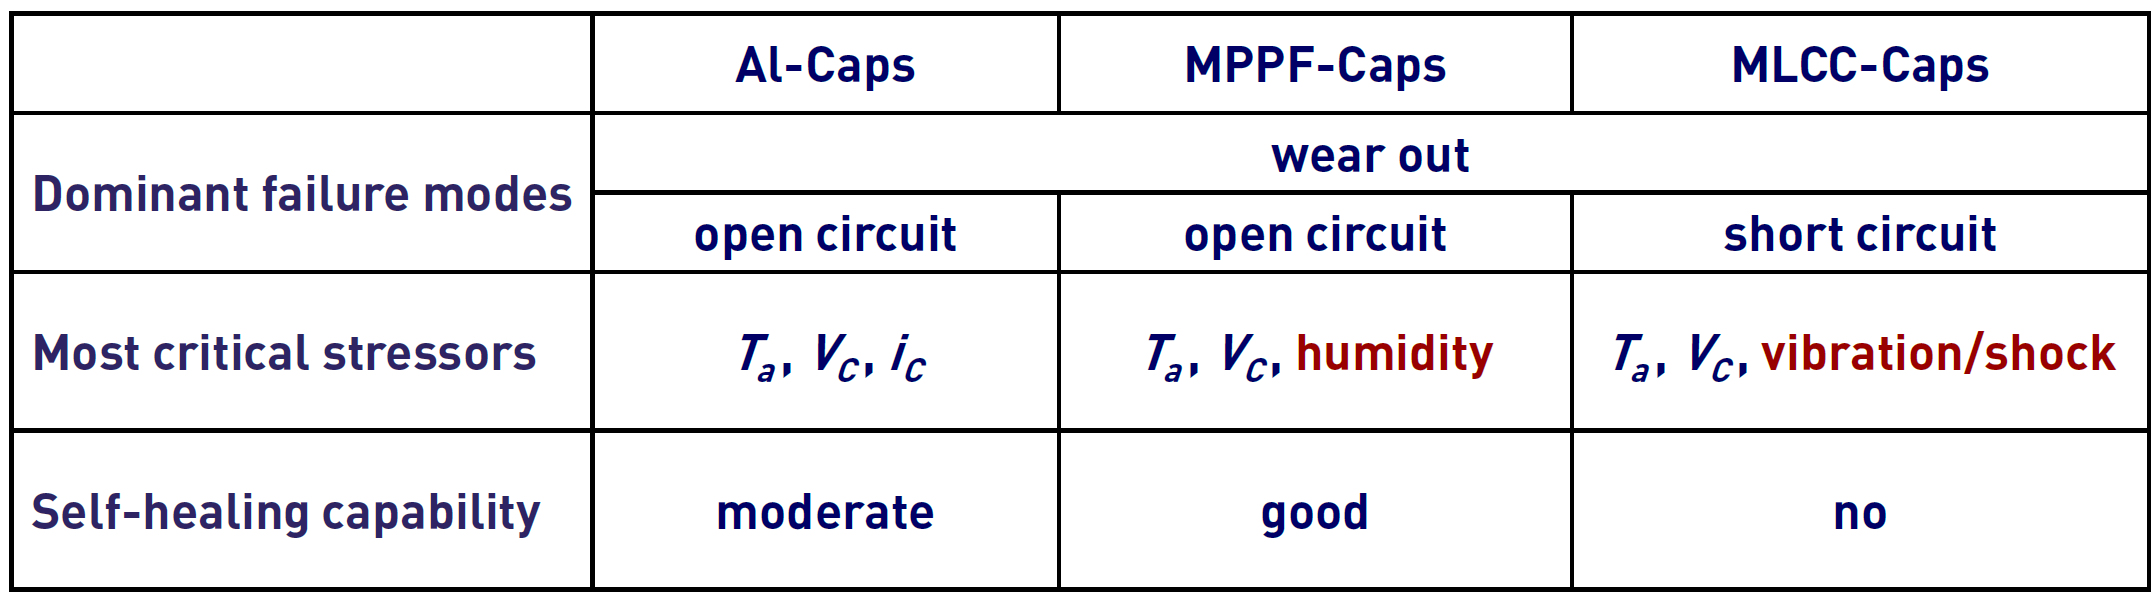
\includegraphics[width=\linewidth]{fig/lec08/failure_summary.png}
    \caption{Summary of dominant failure modes, critical stressors, and self-healing capability for aluminum electrolytic, metallized polypropylene film, and MLCC capacitors. Adapted from Huai Wang, \textit{Capacitors in Power Electronics Applications -- Reliability and Circuit Design}, IECON 2016 tutorial}
\end{figure}
\end{column}
\end{columns}

\end{frame}


%%%%%%%%%%%%%%%%%%%%%%%%%%%%%%%%%%%%%%%%%%%%%%%%%%%%%%%%%%%%%
%% Mission profile based analysis
%%%%%%%%%%%%%%%%%%%%%%%%%%%%%%%%%%%%%%%%%%%%%%%%%%%%%%%%%%%%%
\begin{frame}
\frametitle{Mission-Profile-Based Electro-Thermal Stress Analysis}
\begin{columns}
\begin{column}{0.56\textwidth}
A capacitor does not operate at one fixed condition during its lifetime. It experiences a mission profile. The mission profile includes:
\begin{itemize}
    \item ambient temperature variation,
    \item load power variation,
    \item input voltage variation,
    \item solar irradiance or wind-speed variation,
    \item start--stop cycles,
    \item overload and transient events.
\end{itemize}
\end{column}

\begin{column}{0.40\textwidth}
\begin{figure}
    \centering
    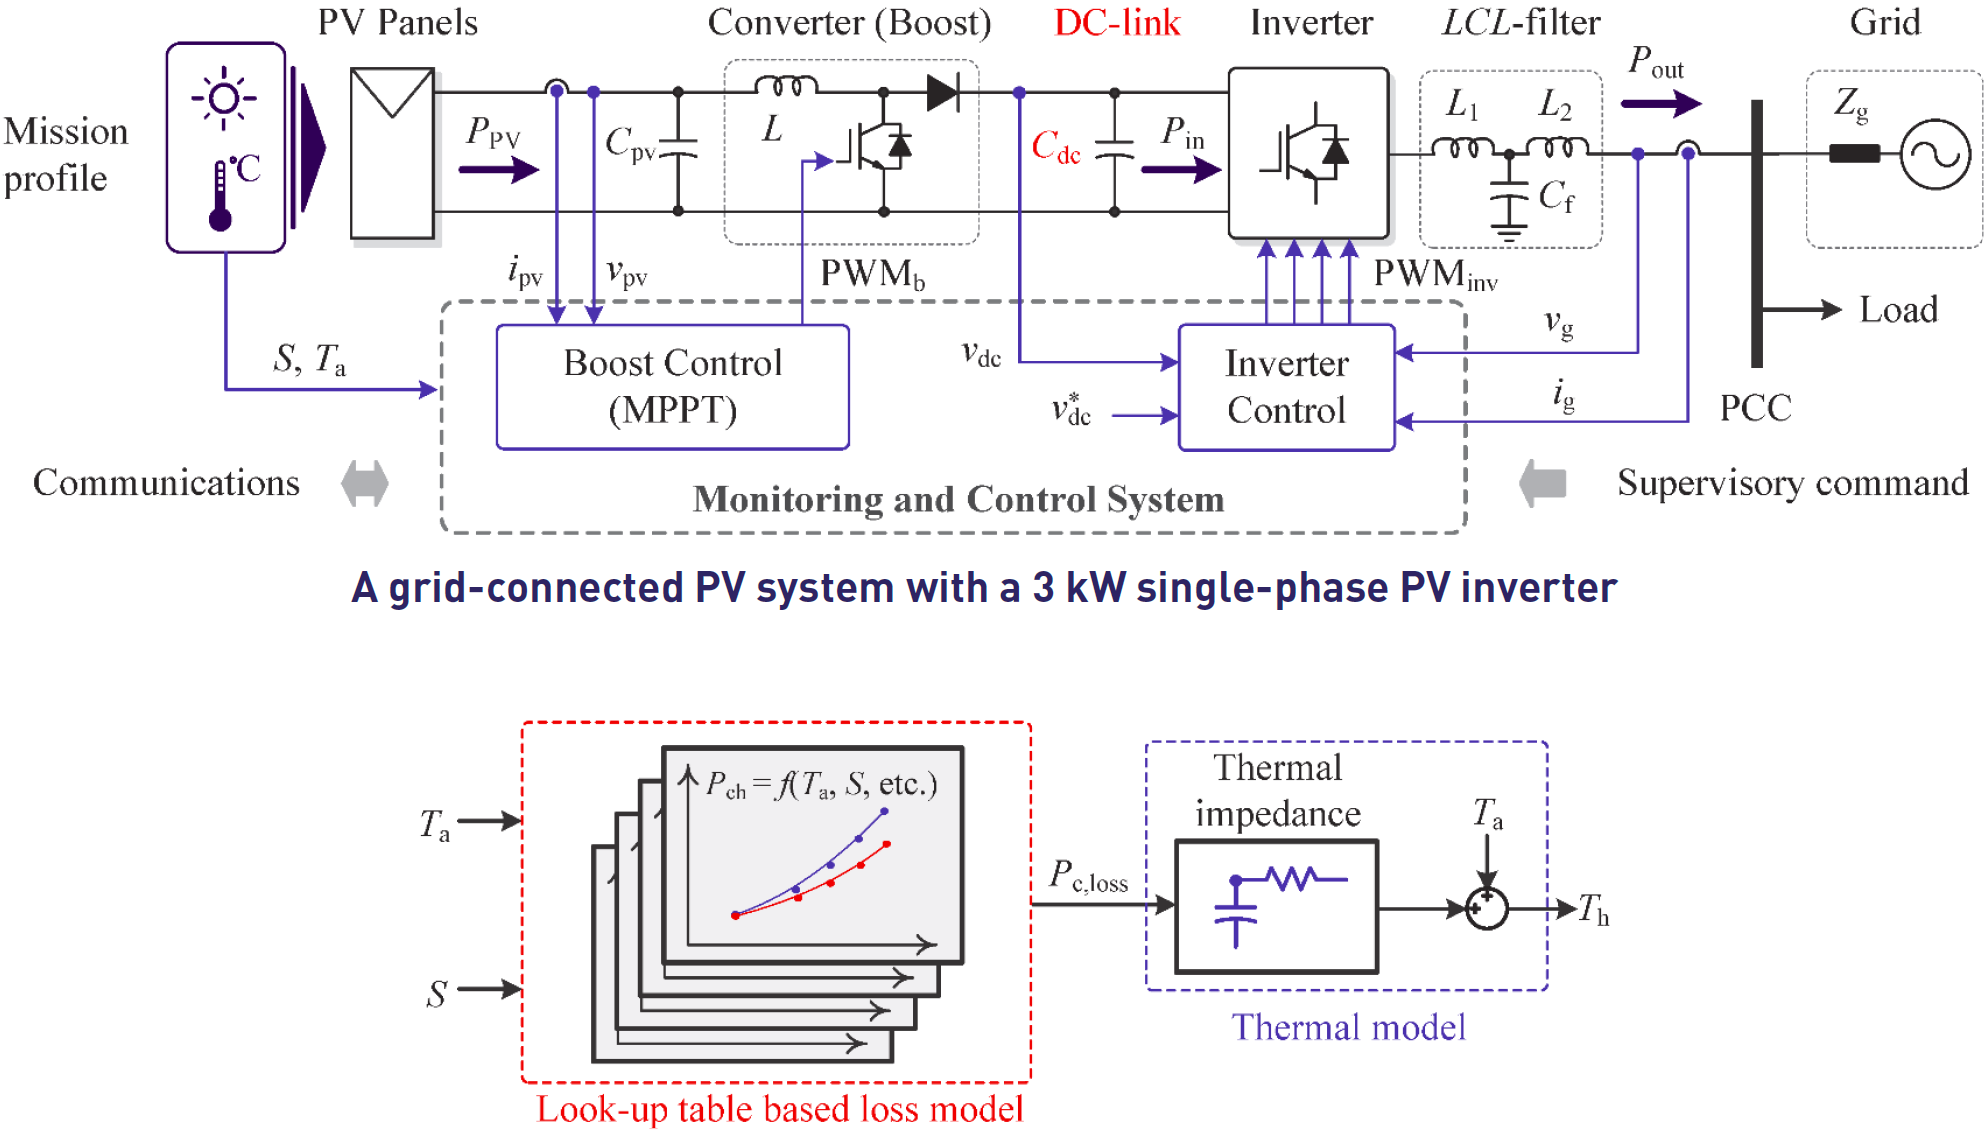
\includegraphics[width=\linewidth]{fig/lec08/mission_profile_model.png}
    \caption{Mission-profile-based electro-thermal modelling workflow for a single-phase PV inverter. Adapted from Huai Wang, \textit{Capacitors in Power Electronics Applications -- Reliability and Circuit Design}, IECON 2016 tutorial}
\end{figure}
\end{column}
\end{columns}

\end{frame}


%%%%%%%%%%%%%%%%%%%%%%%%%%%%%%%%%%%%%%%%%%%%%%%%%%%%%%%%%%%%%
%% Mission profile based analysis
%%%%%%%%%%%%%%%%%%%%%%%%%%%%%%%%%%%%%%%%%%%%%%%%%%%%%%%%%%%%%
\begin{frame}
\frametitle{Mission-Profile-Based Electro-Thermal Stress Analysis}
\begin{columns}
\begin{column}{0.56\textwidth}
The reliability-oriented workflow is:
\begin{enumerate}
    \item translate mission profile into capacitor voltage and current stress,
    \item calculate capacitor losses,
    \item estimate hot-spot temperature,
    \item apply ageing or lifetime model,
    \item accumulate damage over the mission profile.
\end{enumerate}
This approach is essential for PV inverters, EV chargers, railway converters, aircraft systems, and wind-power converters.
\end{column}

\begin{column}{0.40\textwidth}
\begin{figure}
    \centering
    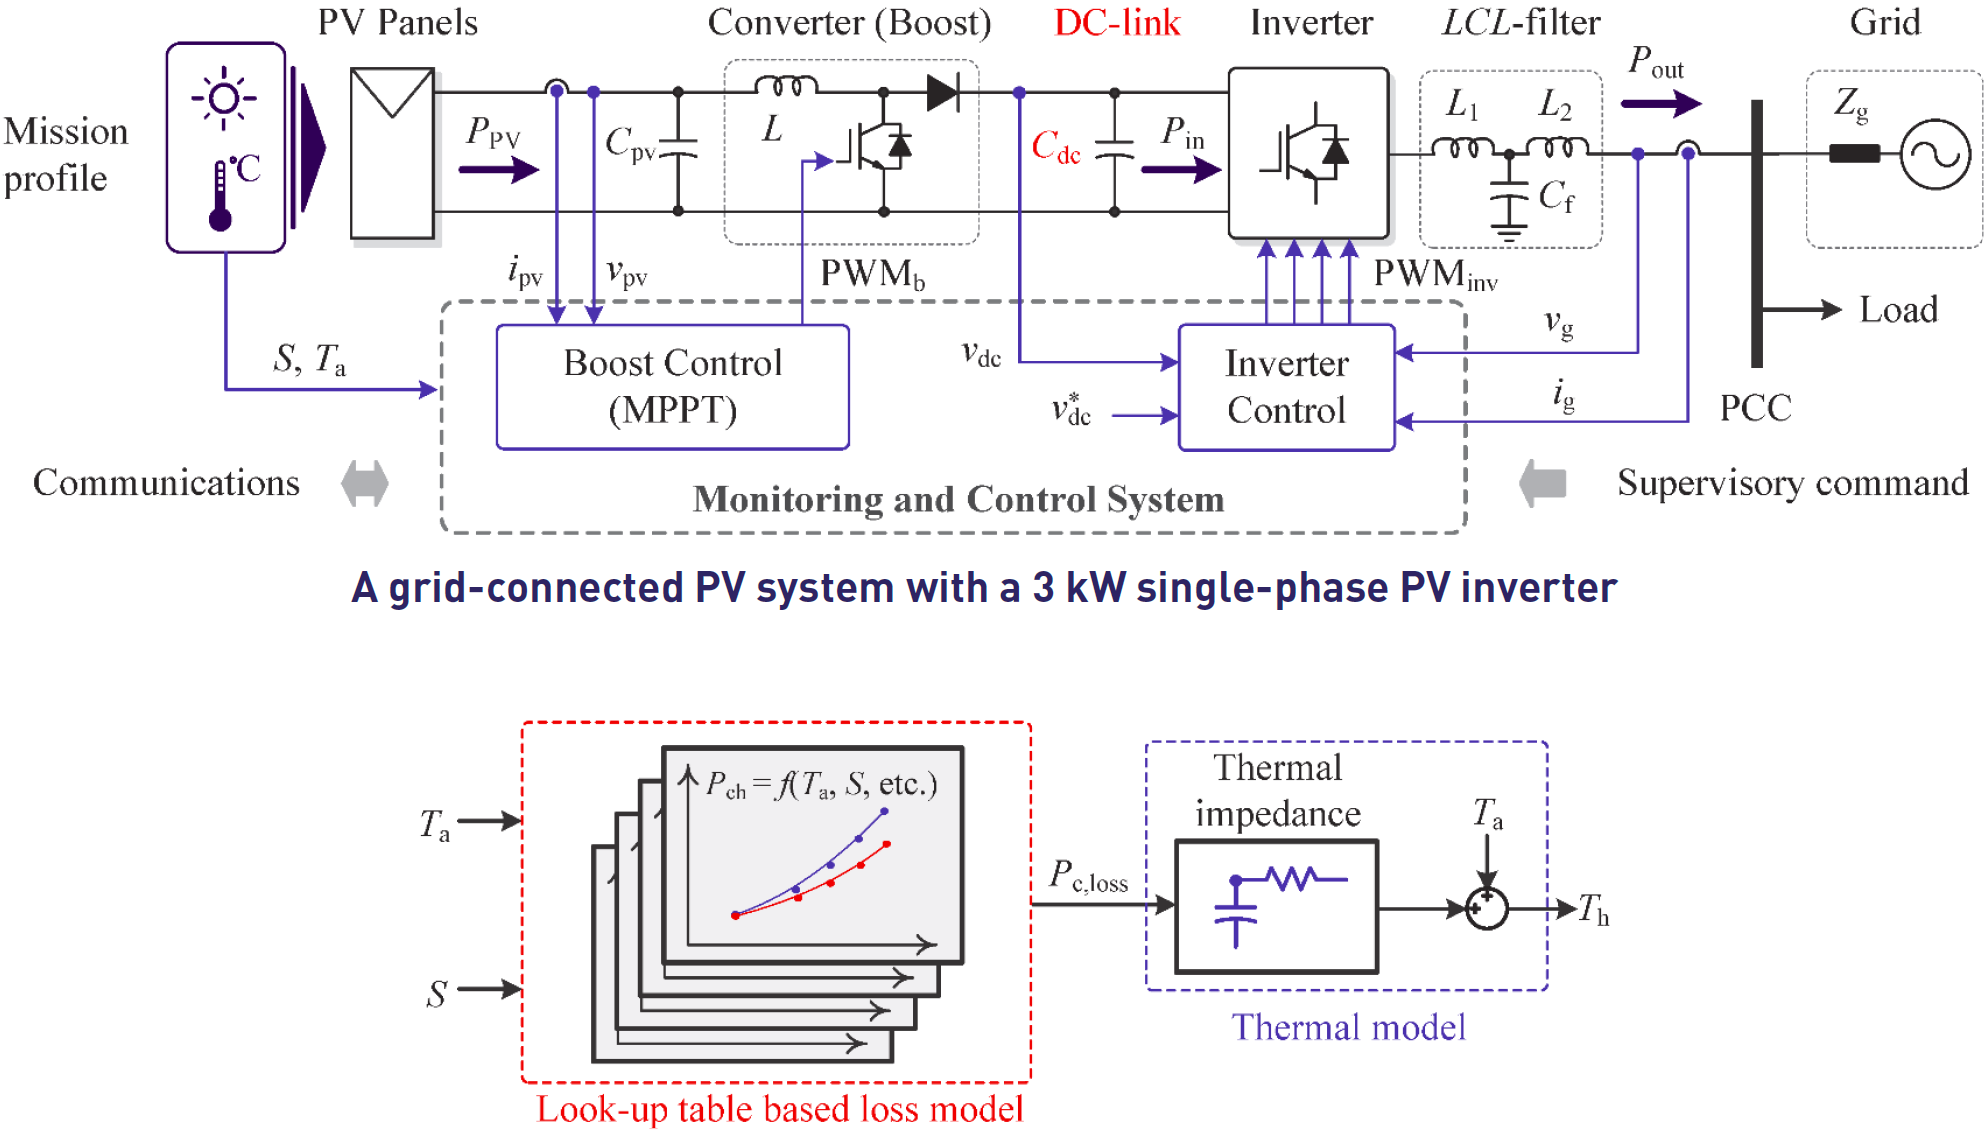
\includegraphics[width=\linewidth]{fig/lec08/mission_profile_model.png}
    \caption{Mission-profile-based electro-thermal modelling workflow for a single-phase PV inverter. Adapted from Huai Wang, \textit{Capacitors in Power Electronics Applications -- Reliability and Circuit Design}, IECON 2016 tutorial}
\end{figure}
\end{column}
\end{columns}

\end{frame}

%%%%%%%%%%%%%%%%%%%%%%%%%%%%%%%%%%%%%%%%%%%%%%%%%%%%%%%%%%%%%
%% Ripple spectrum and temperature stress
%%%%%%%%%%%%%%%%%%%%%%%%%%%%%%%%%%%%%%%%%%%%%%%%%%%%%%%%%%%%%
\begin{frame}
\frametitle{Ripple-Current Spectrum and Temperature Stress}
\begin{columns}
\begin{column}{0.56\textwidth}
In power converters, capacitor current is rarely sinusoidal. It contains many harmonic components. For harmonic currents,

\begin{align}
    I_{\mathrm{rms}}
    =
    \sqrt{
    I_1^2+I_2^2+\cdots+I_n^2
    }
\end{align}

The loss is frequency dependent because ESR changes with frequency:

\begin{align}
    P_{\mathrm{loss}}
    =
    \sum_{k=1}^{n}
    I_k^2
    ESR(f_k)
\end{align}
\end{column}

\begin{column}{0.40\textwidth}
\begin{figure}
    \centering
    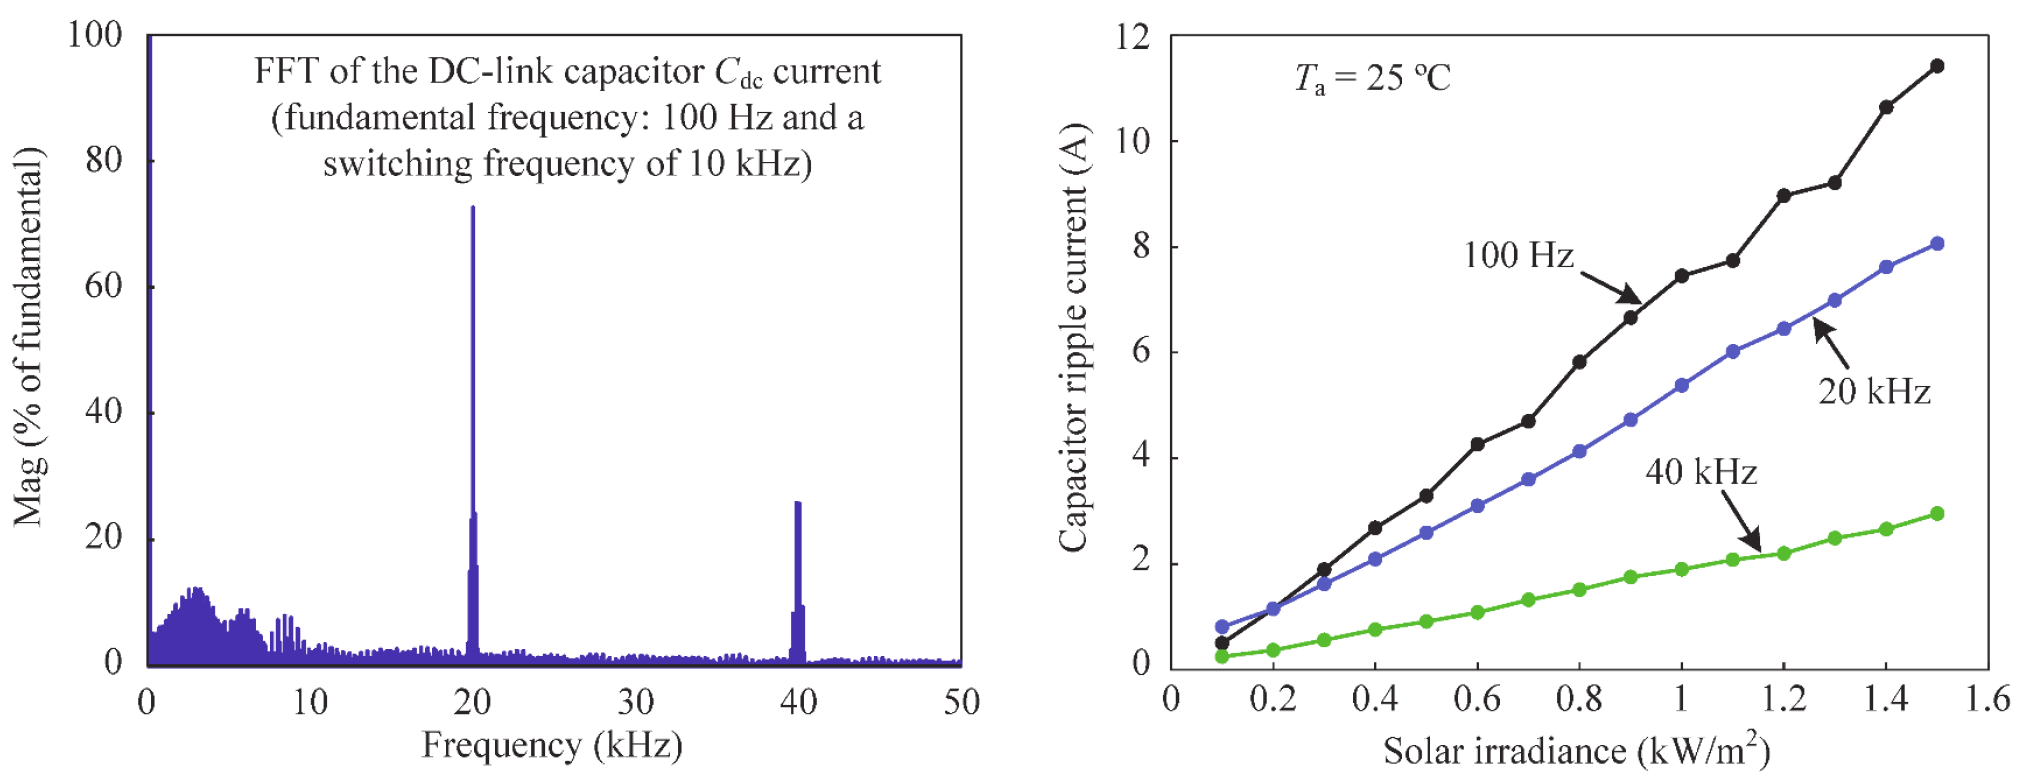
\includegraphics[width=\linewidth]{fig/lec08/ripple_current_spectrum.png}
    \caption{Example ripple-current harmonic spectrum and capacitor ripple currents under different irradiance levels. Adapted from Huai Wang, \textit{Capacitors in Power Electronics Applications -- Reliability and Circuit Design}, IECON 2016 tutorial}
\end{figure}
\end{column}
\end{columns}

\end{frame}


%%%%%%%%%%%%%%%%%%%%%%%%%%%%%%%%%%%%%%%%%%%%%%%%%%%%%%%%%%%%%
%% Ripple spectrum and temperature stress
%%%%%%%%%%%%%%%%%%%%%%%%%%%%%%%%%%%%%%%%%%%%%%%%%%%%%%%%%%%%%
\begin{frame}
\frametitle{Ripple-Current Spectrum and Temperature Stress}
\begin{columns}
\begin{column}{0.56\textwidth}
Ripple spectrum and temperature stress are especially important for:
\begin{itemize}
    \item DC-link capacitors in inverters,
    \item output capacitors in DC--DC converters,
    \item resonant capacitors,
    \item EMI and AC harmonic filter capacitors.
\end{itemize}
A single RMS current number may be insufficient if the frequency spectrum is broad.
\end{column}

\begin{column}{0.40\textwidth}
\begin{figure}
    \centering
    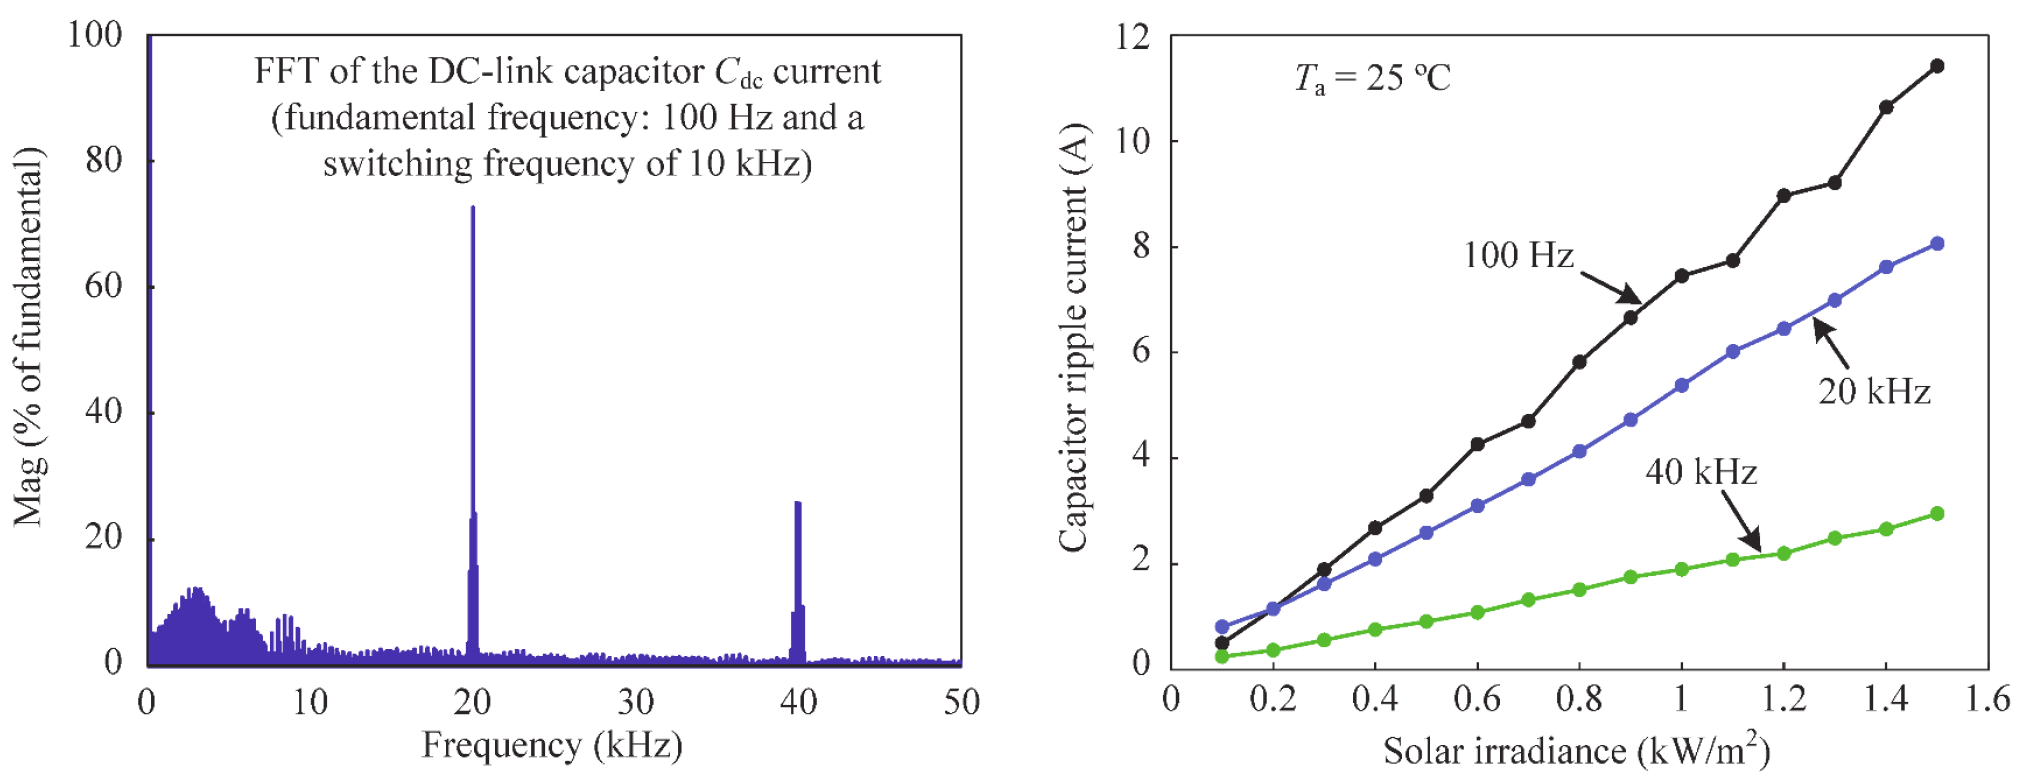
\includegraphics[width=\linewidth]{fig/lec08/ripple_current_spectrum.png}
    \caption{Example ripple-current harmonic spectrum and capacitor ripple currents under different irradiance levels. Adapted from Huai Wang, \textit{Capacitors in Power Electronics Applications -- Reliability and Circuit Design}, IECON 2016 tutorial}
\end{figure}
\end{column}
\end{columns}

\end{frame}

%%%%%%%%%%%%%%%%%%%%%%%%%%%%%%%%%%%%%%%%%%%%%%%%%%%%%%%%%%%%%
%% Humidity degradation film capacitors
%%%%%%%%%%%%%%%%%%%%%%%%%%%%%%%%%%%%%%%%%%%%%%%%%%%%%%%%%%%%%
\begin{frame}
\frametitle{Humidity-Dependent Degradation of Film Capacitors}

\begin{columns}
\begin{column}{0.60\textwidth}
Metallized film capacitors are sensitive to humidity because moisture can degrade the metallization layer. The main effects are:
\begin{itemize}
    \item reduction of active electrode area,
    \item capacitance decrease,
    \item increased dielectric loss,
    \item self-healing activity,
    \item gradual wear-out.
\end{itemize}
In accelerated tests, end-of-life can be defined by a specified capacitance drop, for example \(5\%\) reduction.

For PV inverters and outdoor converters, humidity stress must be considered with voltage, temperature, and ripple current.
\end{column}

\begin{column}{0.40\textwidth}
        \vspace{-0.5cm}
\begin{figure}
    \centering
    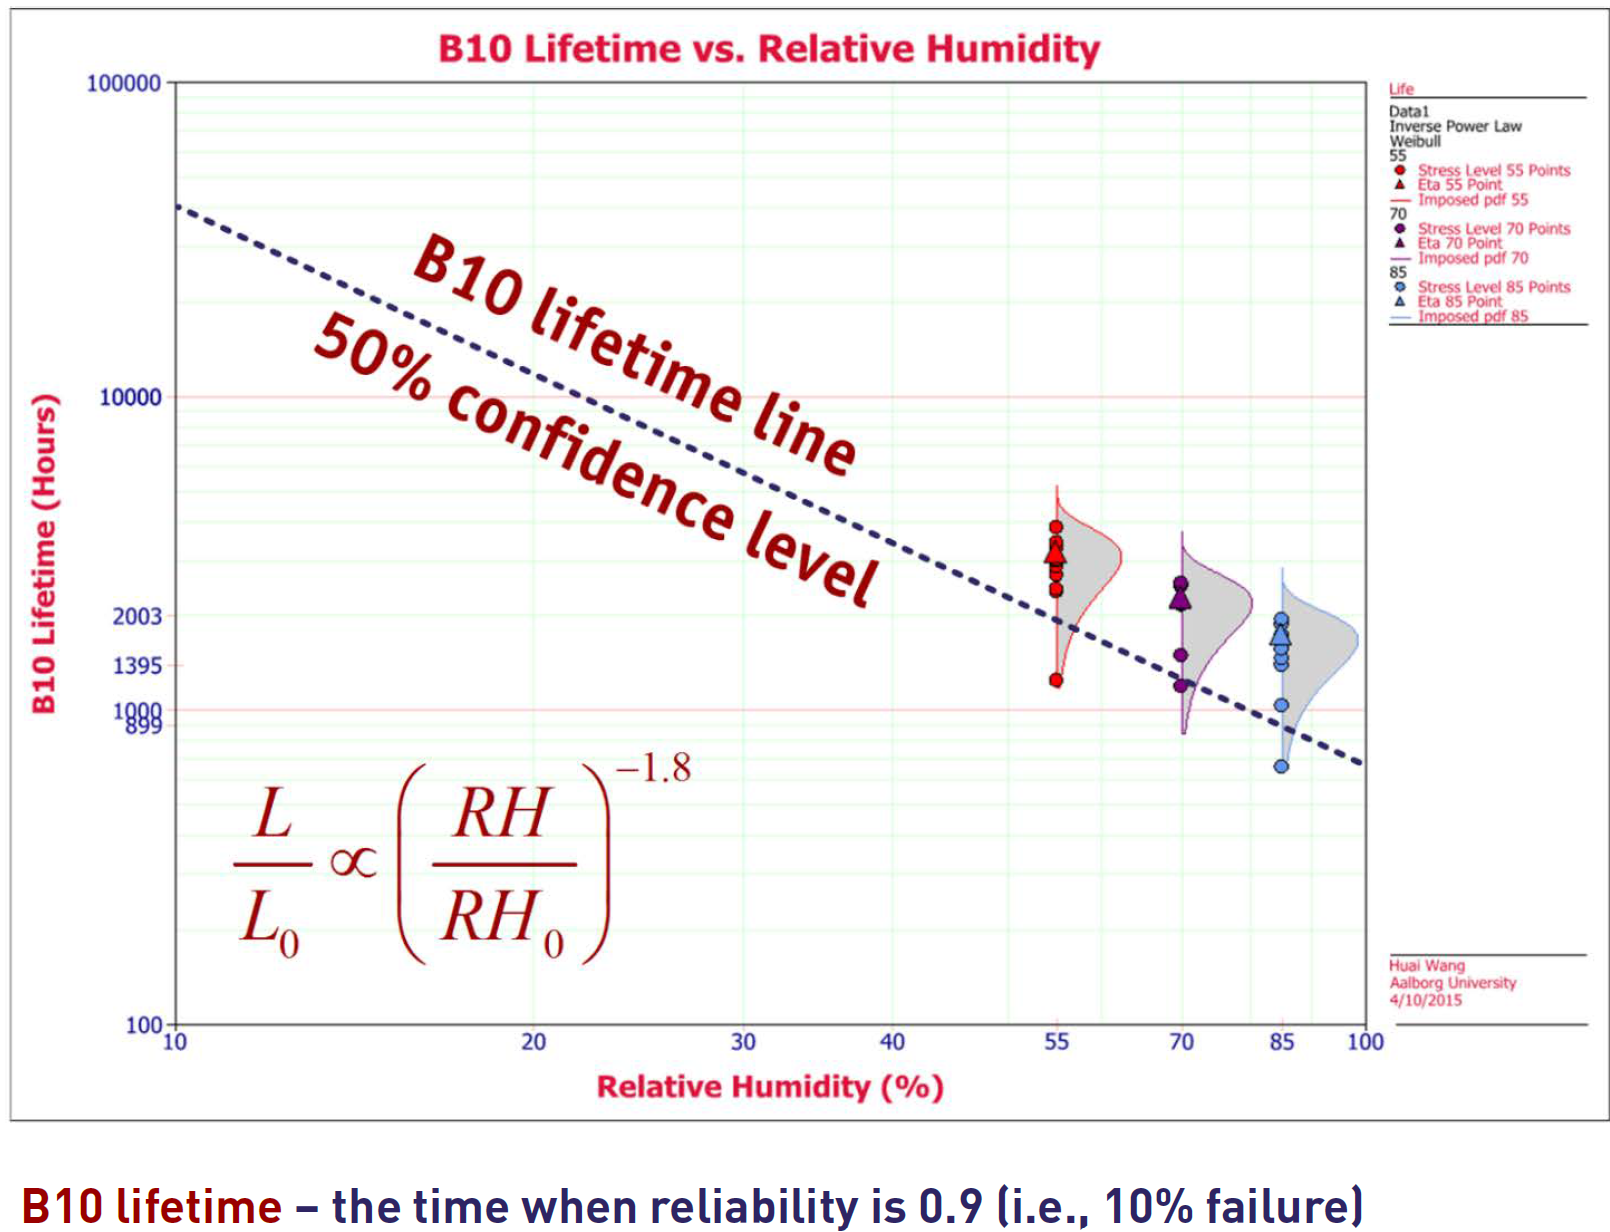
\includegraphics[width=\linewidth]{fig/lec08/humidity_lifetime_MPPF.png}
    \caption{Humidity-dependent lifetime of metallized polypropylene film capacitors under accelerated ageing conditions. Adapted from Huai Wang, \textit{Capacitors in Power Electronics Applications -- Reliability and Circuit Design}, IECON 2016 tutorial}
\end{figure}
\end{column}
\end{columns}

\end{frame}


%%%%%%%%%%%%%%%%%%%%%%%%%%%%%%%%%%%%%%%%%%%%%%%%%%%%%%%%%%%%%
%% Condition monitoring
%%%%%%%%%%%%%%%%%%%%%%%%%%%%%%%%%%%%%%%%%%%%%%%%%%%%%%%%%%%%%
\begin{frame}
\frametitle{Condition Monitoring of Capacitors}
\begin{columns}
\begin{column}{0.56\textwidth}
Condition monitoring aims to estimate the health of a capacitor during converter operation.Useful health indicators include:
\begin{itemize}
    \item capacitance \(C\),
    \item ESR,
    \item dissipation factor \(\tan\delta\),
    \item leakage current \(I_{\mathrm{LC}}\),
    \item insulation resistance \(R_p\),
    \item hot-spot temperature,
    \item ripple-current stress.
\end{itemize}
\end{column}

\begin{column}{0.45\textwidth}
        \vspace{-1cm}
\begin{figure}
    \centering
    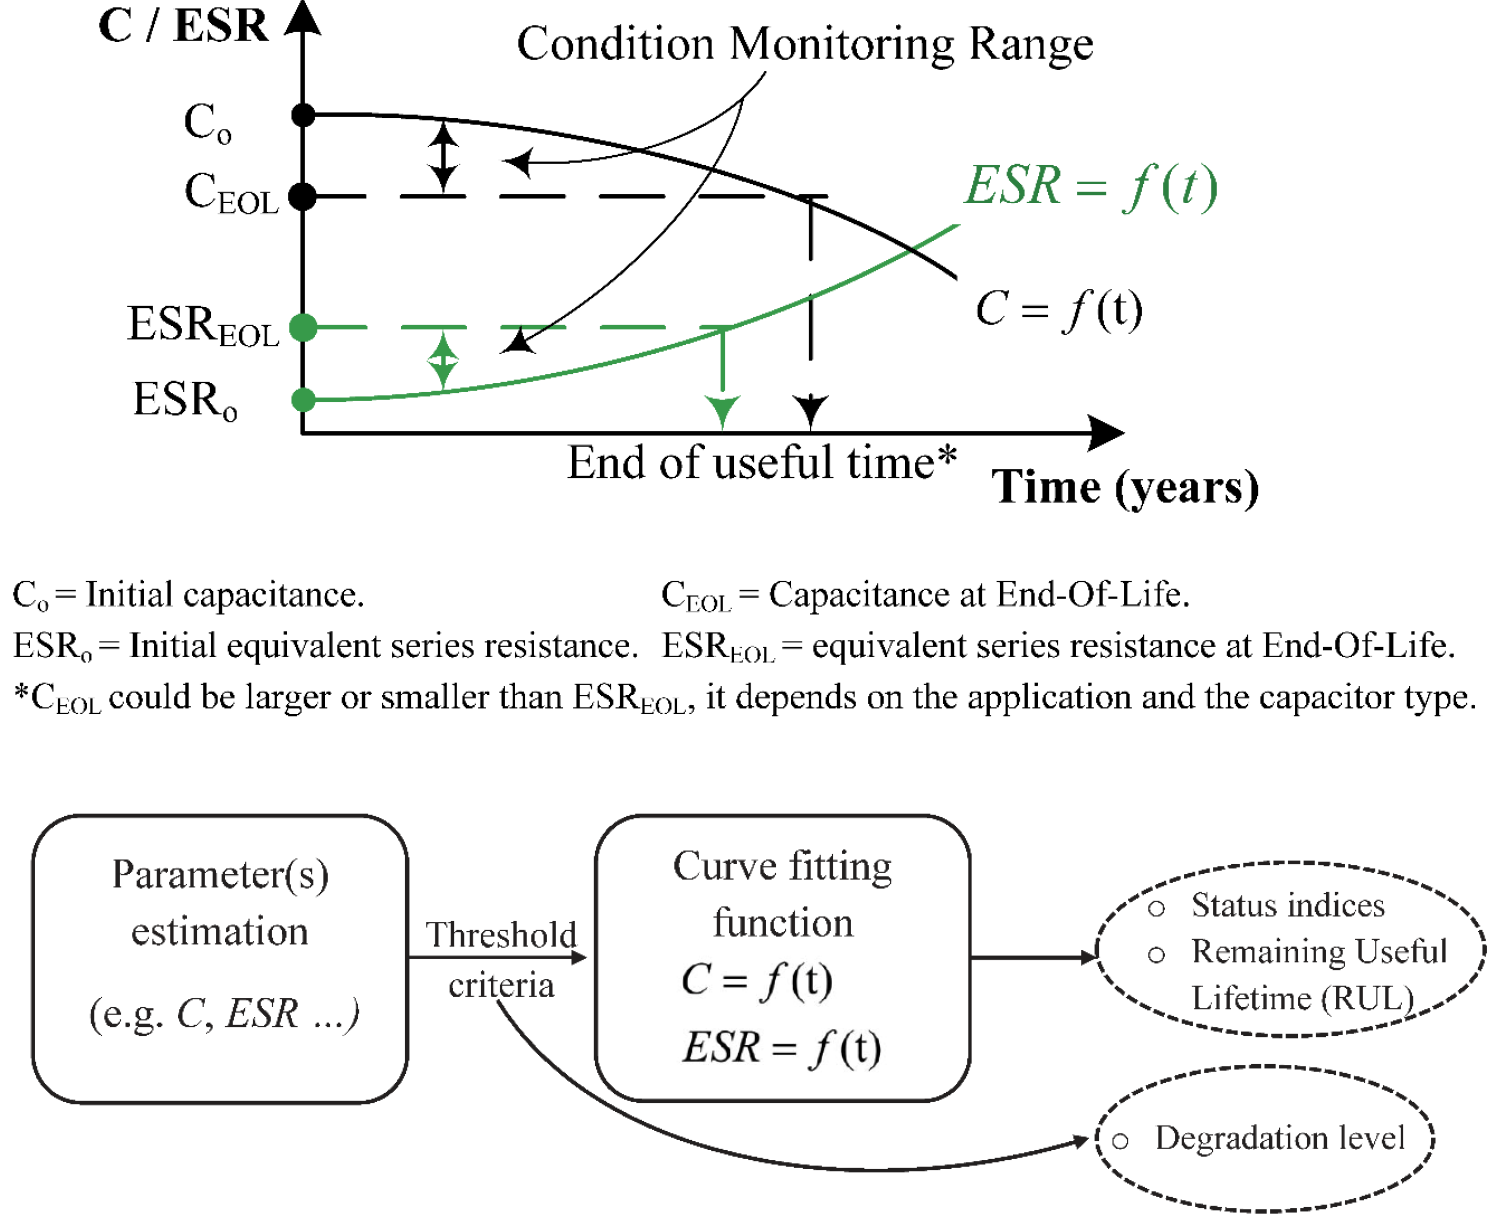
\includegraphics[width=\linewidth]{fig/lec08/condition_indicators.png}
    \caption{Key indicators for capacitor condition monitoring: capacitance, ESR, \(\tan\delta\), leakage current and insulation resistance. Adapted from Huai Wang, \textit{Capacitors in Power Electronics Applications -- Reliability and Circuit Design}, IECON 2016 tutorial}
\end{figure}
\end{column}
\end{columns}

\end{frame}


%%%%%%%%%%%%%%%%%%%%%%%%%%%%%%%%%%%%%%%%%%%%%%%%%%%%%%%%%%%%%
%% Condition monitoring
%%%%%%%%%%%%%%%%%%%%%%%%%%%%%%%%%%%%%%%%%%%%%%%%%%%%%%%%%%%%%
\begin{frame}
\frametitle{Condition Monitoring of Capacitors}
\begin{columns}
\begin{column}{0.56\textwidth}
Typical ageing trends:
\begin{itemize}
    \item electrolytic capacitors: ESR increases and capacitance decreases,
    \item film capacitors: capacitance decreases due to metallization loss,
    \item MLCCs: insulation degradation or cracking may produce sudden failure.
\end{itemize}
Online monitoring is particularly valuable for DC-link capacitors in long-life converters.

\end{column}

\begin{column}{0.45\textwidth}
    \vspace{-1cm}
\begin{figure}
    \centering
    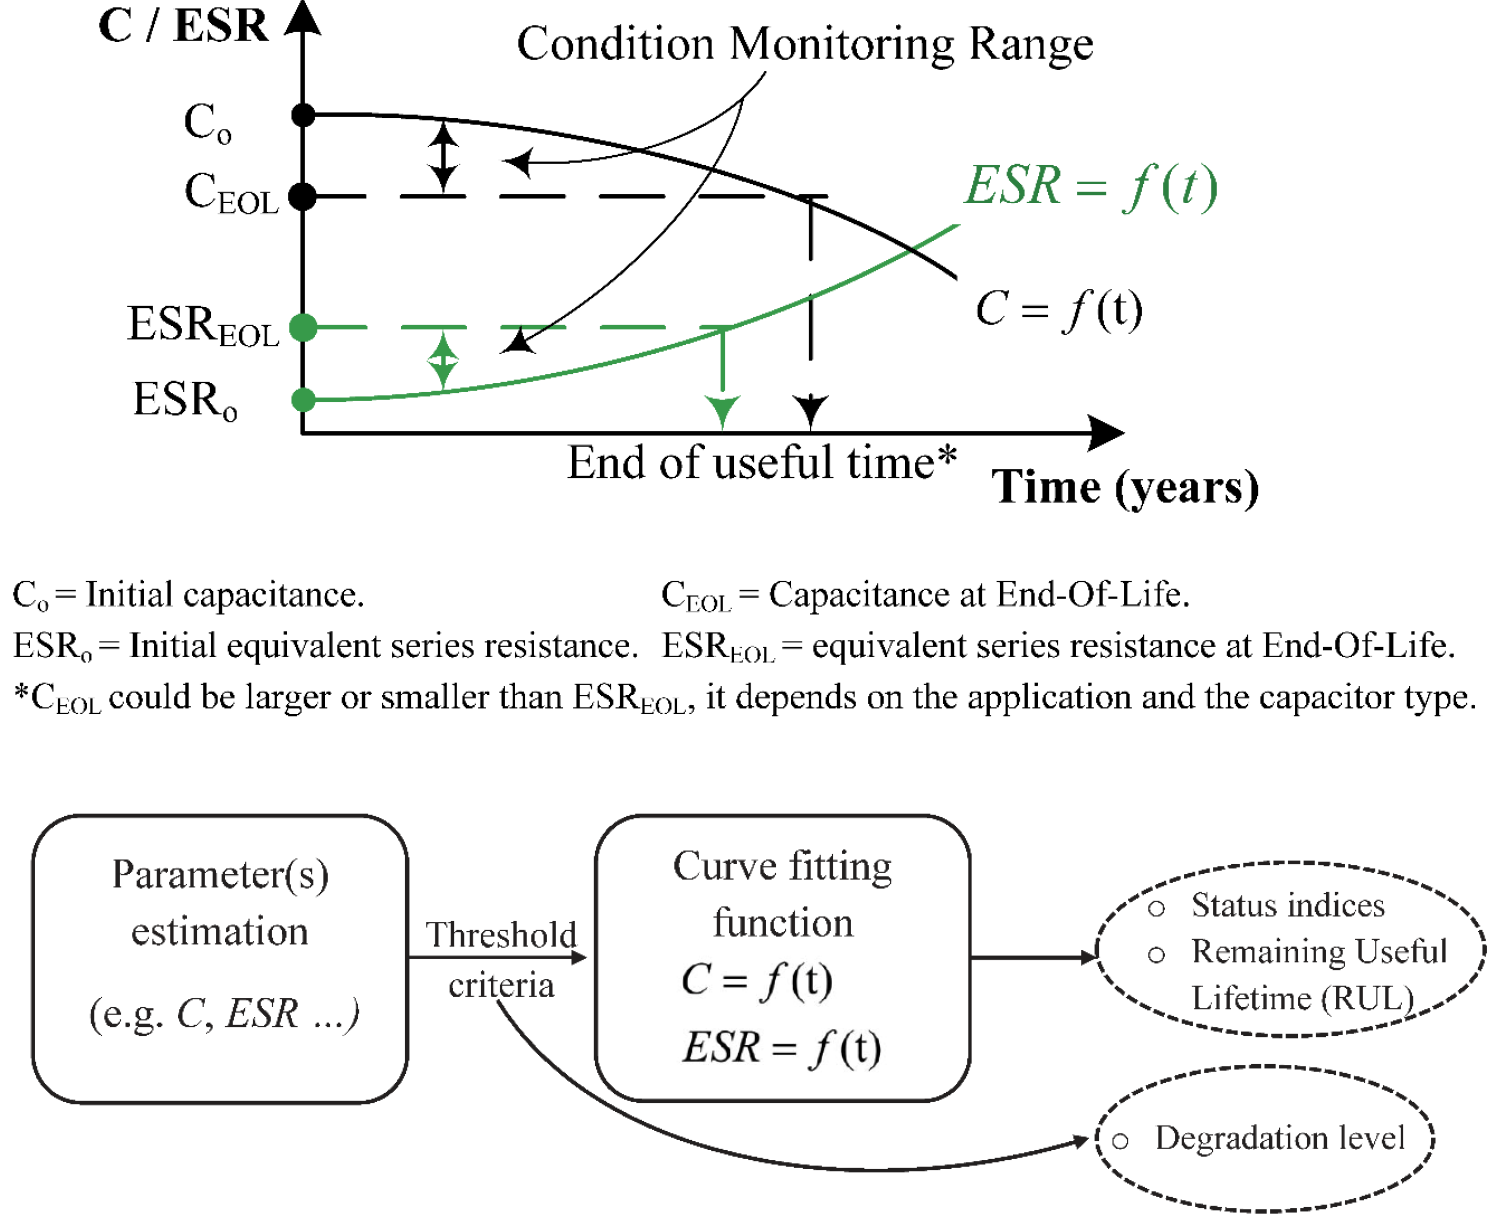
\includegraphics[width=\linewidth]{fig/lec08/condition_indicators.png}
    \caption{Key indicators for capacitor condition monitoring: capacitance, ESR, \(\tan\delta\), leakage current and insulation resistance. Adapted from Huai Wang, \textit{Capacitors in Power Electronics Applications -- Reliability and Circuit Design}, IECON 2016 tutorial}
\end{figure}
\end{column}
\end{columns}

\end{frame}

%%%%%%%%%%%%%%%%%%%%%%%%%%%%%%%%%%%%%%%%%%%%%%%%%%%%%%%%%%%%%
%% ESR estimation
%%%%%%%%%%%%%%%%%%%%%%%%%%%%%%%%%%%%%%%%%%%%%%%%%%%%%%%%%%%%%
\begin{frame}
\frametitle{Online ESR Estimation}
\begin{columns}
\begin{column}{0.56\textwidth}
A common online health-monitoring method estimates the ESR of the DC-link capacitor. The basic idea is that ESR creates a voltage ripple proportional to capacitor current:

\begin{align}
    v_{\mathrm{ESR}}(t)
    =
    i_C(t)R_{\mathrm{ESR}}
\end{align}
Thus, if capacitor current and ripple voltage are known or estimated,
\begin{align}
    R_{\mathrm{ESR}}
    \approx
    \frac{v_{\mathrm{ripple}}}{i_{\mathrm{ripple}}}
\end{align}
\end{column}

\begin{column}{0.40\textwidth}
\begin{figure}
    \centering
    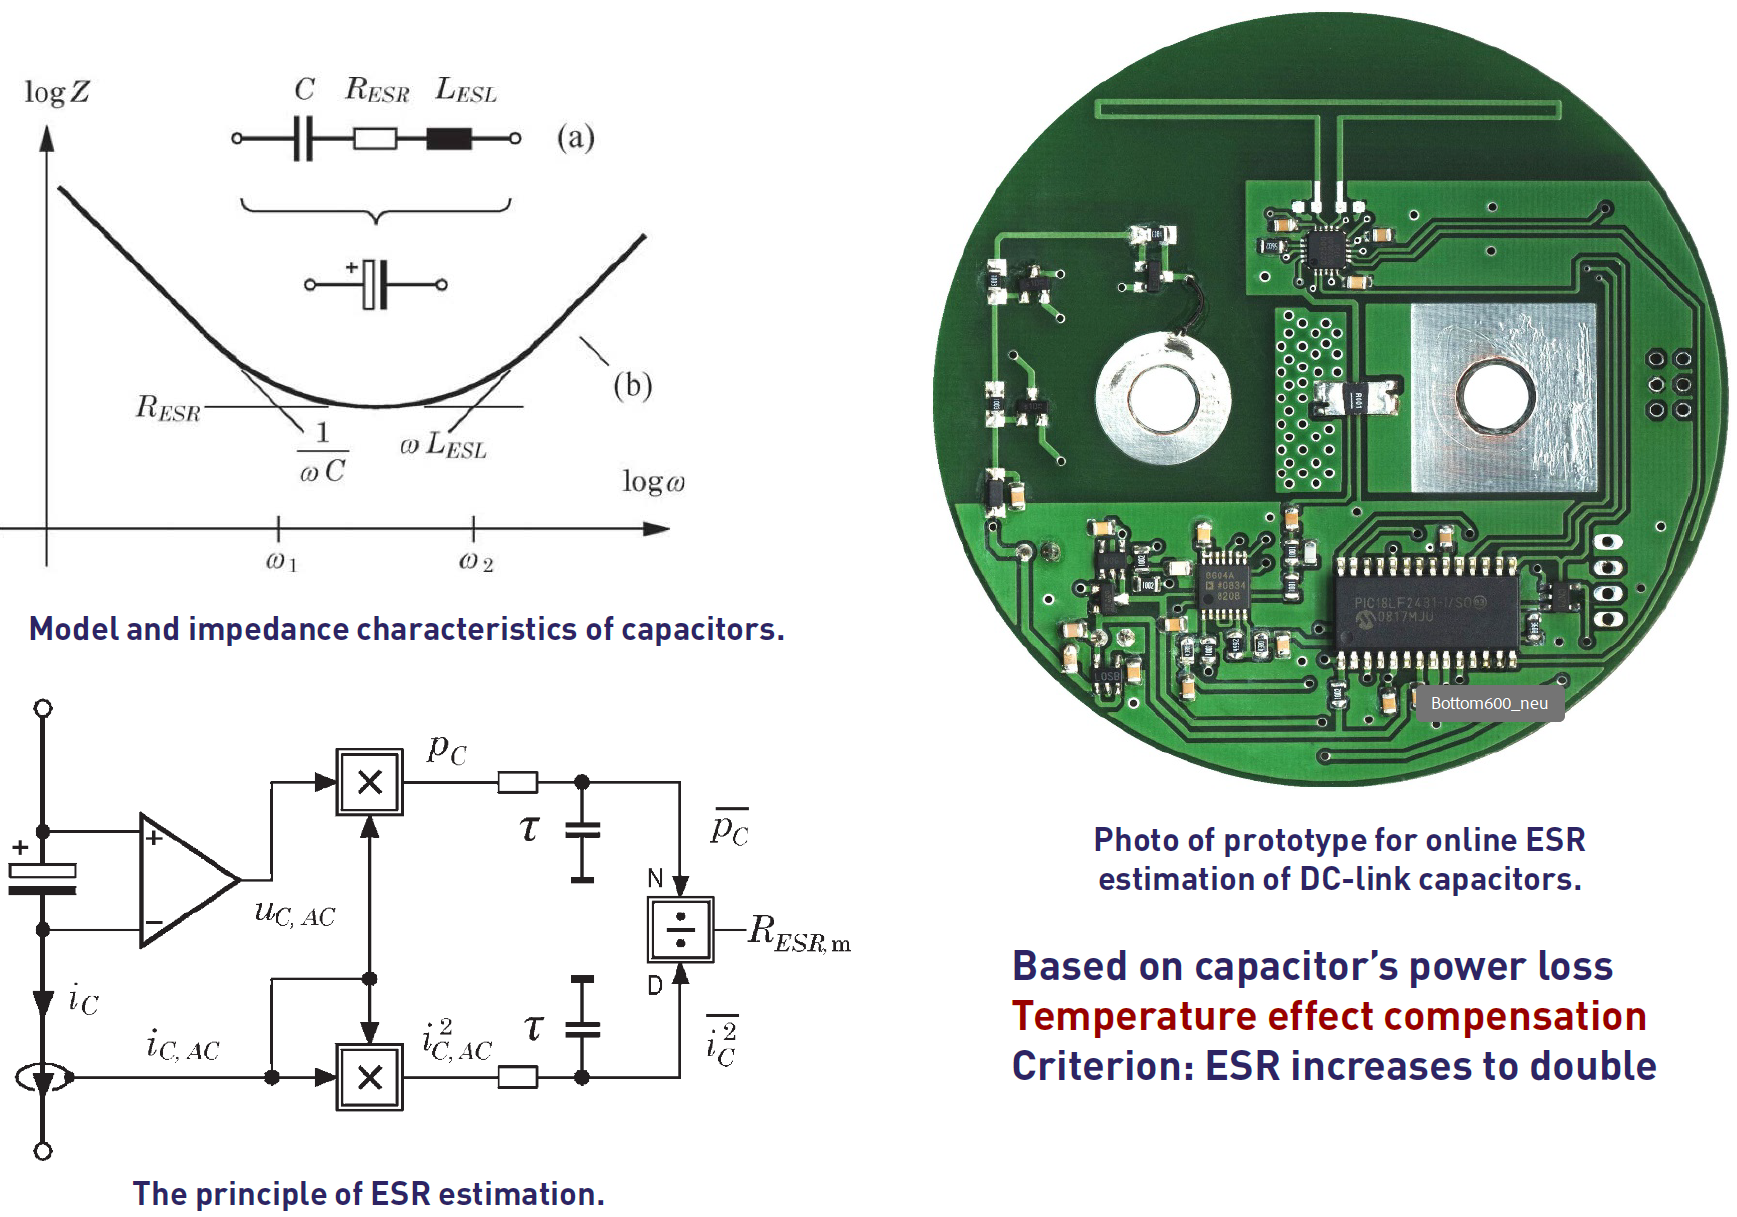
\includegraphics[width=\linewidth]{fig/lec08/online_ESR_estimation.png}
    \caption{Prototype and principle for online ESR estimation of DC-link capacitors, including temperature compensation. Adapted from Huai Wang, \textit{Capacitors in Power Electronics Applications -- Reliability and Circuit Design}, IECON 2016 tutorial}
\end{figure}
\end{column}
\end{columns}

\end{frame}


%%%%%%%%%%%%%%%%%%%%%%%%%%%%%%%%%%%%%%%%%%%%%%%%%%%%%%%%%%%%%
%% ESR estimation
%%%%%%%%%%%%%%%%%%%%%%%%%%%%%%%%%%%%%%%%%%%%%%%%%%%%%%%%%%%%%
\begin{frame}
\frametitle{Online ESR Estimation}
\begin{columns}
\begin{column}{0.56\textwidth}
However, practical ESR estimation must compensate for:
\begin{itemize}
    \item temperature dependence,
    \item frequency dependence,
    \item measurement noise,
    \item non-ESR ripple components,
    \item converter operating-point variation.
\end{itemize}
A typical end-of-life criterion for electrolytic capacitors is ESR increasing to a specified multiple of its initial value.
\end{column}

\begin{column}{0.40\textwidth}
\begin{figure}
    \centering
    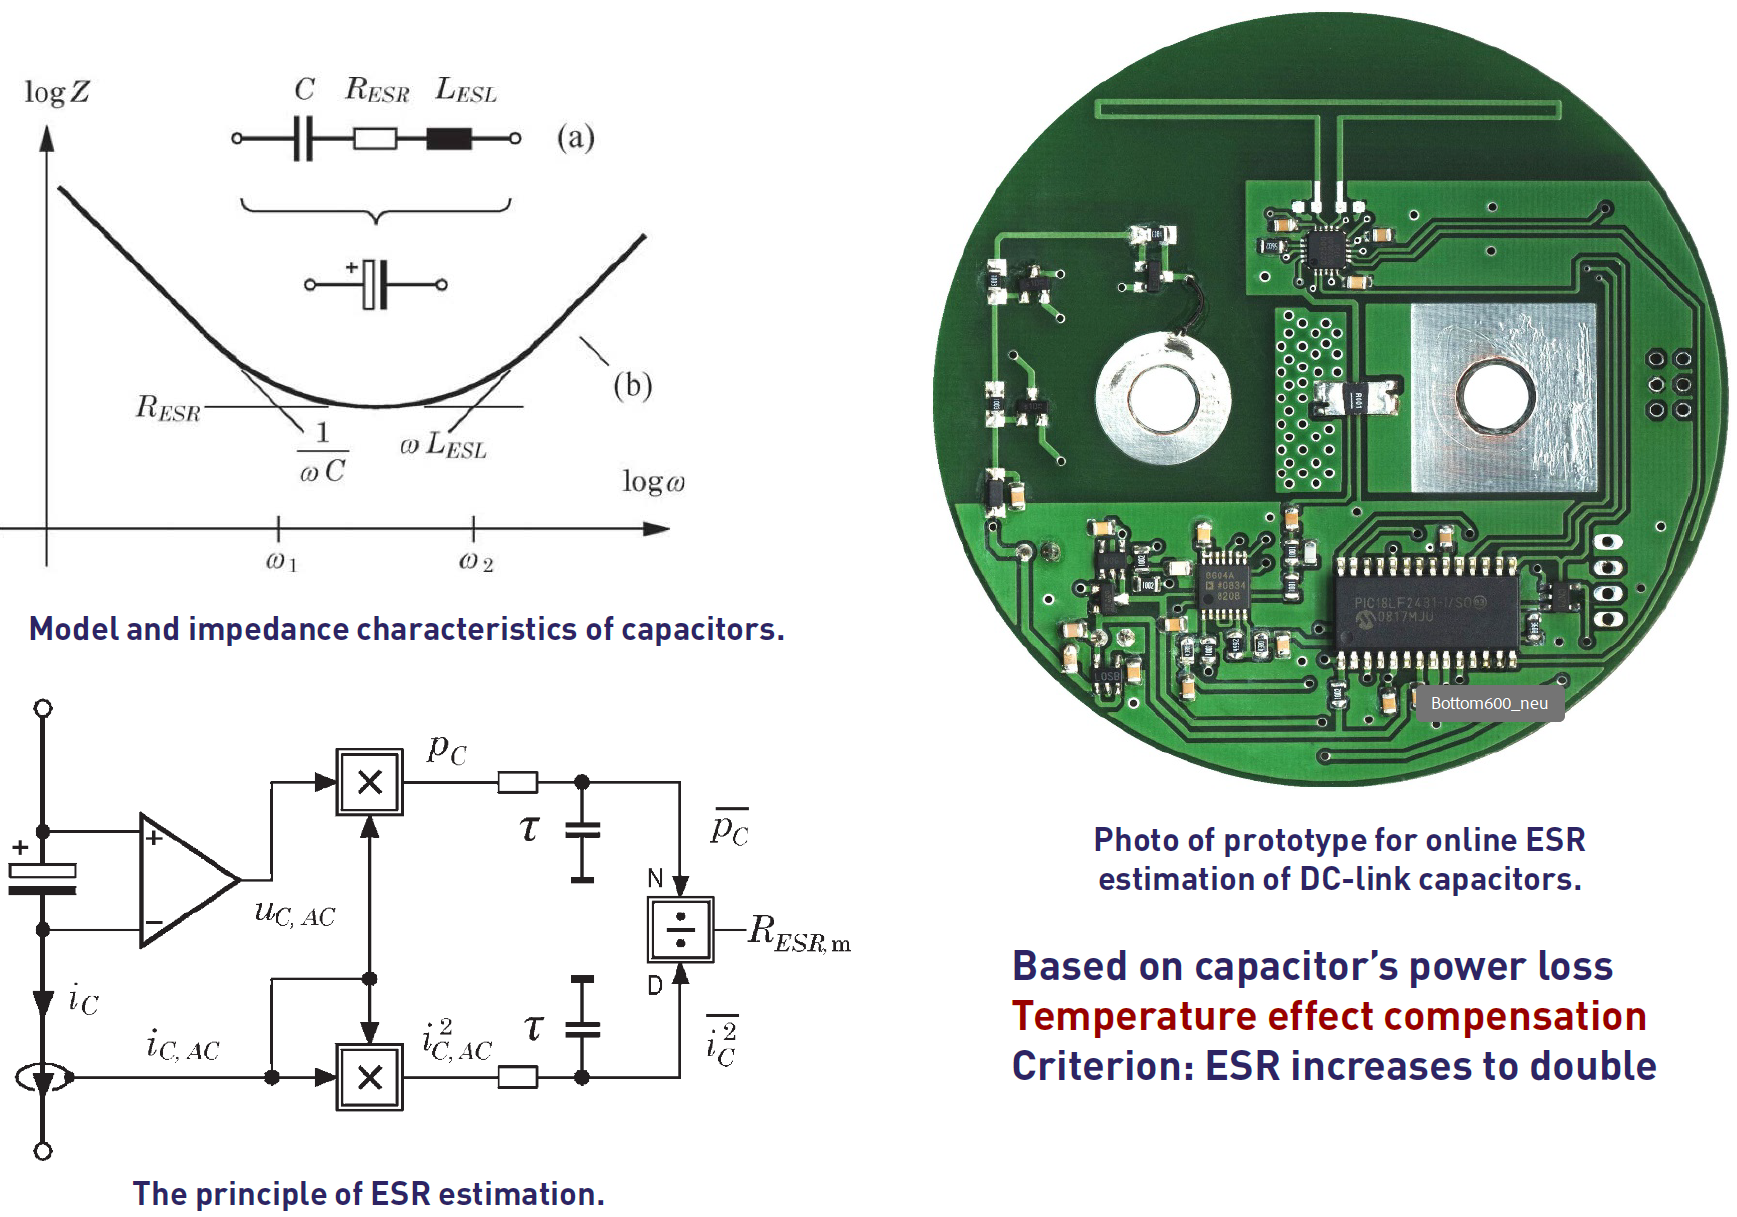
\includegraphics[width=\linewidth]{fig/lec08/online_ESR_estimation.png}
    \caption{Prototype and principle for online ESR estimation of DC-link capacitors, including temperature compensation. Adapted from Huai Wang, \textit{Capacitors in Power Electronics Applications -- Reliability and Circuit Design}, IECON 2016 tutorial}
\end{figure}
\end{column}
\end{columns}
\end{frame}


%%%%%%%%%%%%%%%%%%%%%%%%%%%%%%%%%%%%%%%%%%%%%%%%%%%%%%%%%%%%%
%% Remaining lifetime prediction
%%%%%%%%%%%%%%%%%%%%%%%%%%%%%%%%%%%%%%%%%%%%%%%%%%%%%%%%%%%%%
\begin{frame}
\frametitle{Remaining Lifetime Prediction}
Remaining lifetime prediction combines condition monitoring with ageing models. A general workflow is:

\begin{enumerate}
    \item measure or estimate capacitor stress:
    \[
        V_C,\; i_C,\; T_{\mathrm{hotspot}}
    \]

    \item estimate health indicators:
    \[
        C,\; ESR,\; \tan\delta,\; I_{\mathrm{LC}}
    \]

    \item compare with degradation model,

    \item predict time to end-of-life criterion.
\end{enumerate}
Relevant for converters where capacitor replacement is expensive or difficult, such as:
\begin{itemize}
    \item offshore wind converters,
    \item railway converters,
    \item PV inverters,
    \item aircraft power systems,
    \item EV fast chargers.
\end{itemize}

\end{frame}


%%%%%%%%%%%%%%%%%%%%%%%%%%%%%%%%%%%%%%%%%%%%%%%%%%%%%%%%%%%%%
%% Common design mistakes
%%%%%%%%%%%%%%%%%%%%%%%%%%%%%%%%%%%%%%%%%%%%%%%%%%%%%%%%%%%%%
\begin{frame}
\frametitle{Common Capacitor Design Mistakes}

\begin{itemize}
    \item Selecting the capacitor only by nominal capacitance.

    \item Ignoring effective MLCC capacitance reduction under DC bias.

    \item Checking voltage rating but not ripple-current rating.

    \item Assuming RMS current sharing is equal in a parallel capacitor bank.

    \item Ignoring ESR variation with temperature, frequency and ageing.

    \item Ignoring ESL and external loop inductance in fast SiC/GaN converters.

    \item Using bulk electrolytics for high-frequency decoupling without local ceramic or film capacitors.

    \item Omitting discharge resistors or safe discharge verification in high-voltage DC links.

    \item Neglecting humidity effects in metallized film capacitors used in outdoor converters.

    \item Estimating lifetime from ambient temperature instead of capacitor hot-spot temperature.

    \item Ignoring mechanical stress, board flex, and cracking risk for MLCCs.
\end{itemize}

\end{frame}


%%%%%%%%%%%%%%%%%%%%%%%%%%%%%%%%%%%%%%%%%%%%%%%%%%%%%%%%%%%%%
%% Capacitors for WBG converters
%%%%%%%%%%%%%%%%%%%%%%%%%%%%%%%%%%%%%%%%%%%%%%%%%%%%%%%%%%%%%
\begin{frame}
\frametitle{Capacitors for SiC and GaN Power Electronics}
SiC and GaN devices enable high switching frequency and very fast voltage/current transitions. This changes capacitor requirements significantly. Important requirements are:

\begin{itemize}
    \item very low ESL,
    \item high RMS and peak current density,
    \item high \(dv/dt\) capability,
    \item high-temperature operation,
    \item compact placement close to the switching cell,
    \item low-loss operation at hundreds of kHz to MHz,
    \item compatibility with laminated busbars or embedded PCB structures.
\end{itemize}

The capacitor must be co-designed with the power module and layout. Otherwise, the switching speed advantage of WBG devices is lost to ringing, overshoot, EMI and thermal stress.

\end{frame}


%%%%%%%%%%%%%%%%%%%%%%%%%%%%%%%%%%%%%%%%%%%%%%%%%%%%%%%%%%%%%
%% Integrated capacitors in WBG modules
%%%%%%%%%%%%%%%%%%%%%%%%%%%%%%%%%%%%%%%%%%%%%%%%%%%%%%%%%%%%%
\begin{frame}
\frametitle{Integrated DC-Link and Snubber Capacitors}
\begin{columns}
\begin{column}{0.56\textwidth}
Capacitor integration minimizes commutation-loop inductance:
\begin{align}
    v_{\sigma}
    =
    L_{\sigma}
    \frac{di}{dt}
\end{align}
Integration strategies:
\begin{itemize}
    \item ceramic capacitors mounted directly on the power module,
    \item capacitors embedded into PCB or busbar,
    \item laminated busbars with field cancellation,
    \item snubber capacitors across switching devices,
    \item film bulk capacitors with local ceramic HF capacitors.
\end{itemize}
\end{column}

\begin{column}{0.40\textwidth}
\begin{figure}
    \centering
    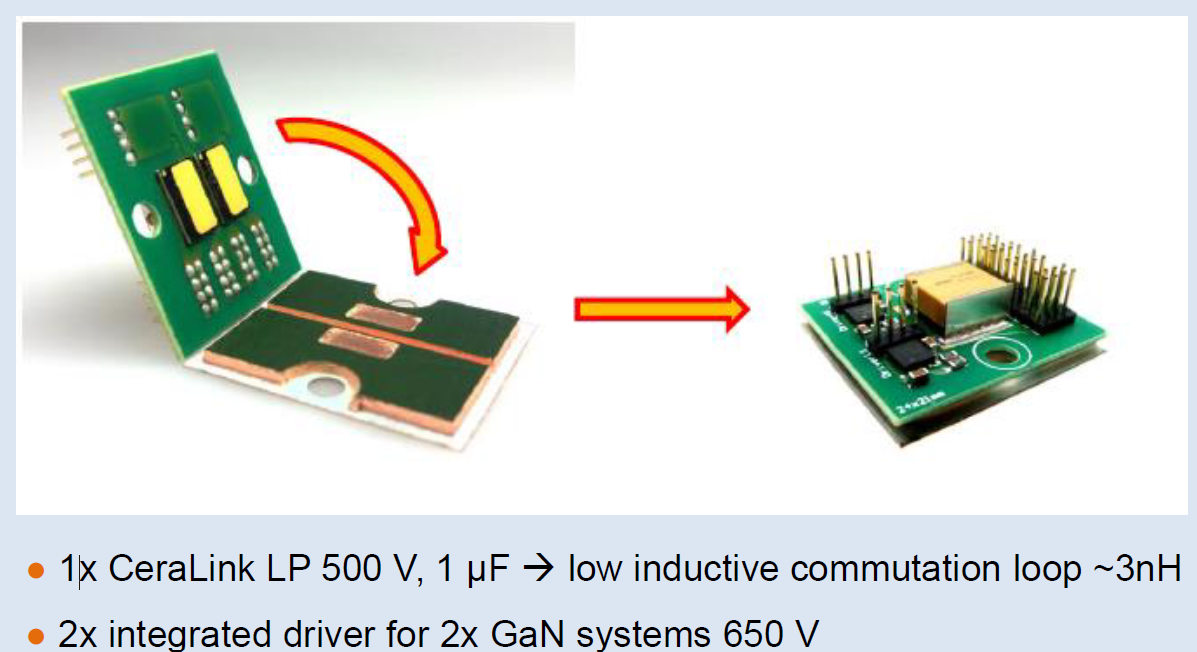
\includegraphics[width=\linewidth]{fig/lec08/GaN_integrated_DC_link.png}
    \caption{GaN power module with integrated driver and DC-link capacitors using low-inductance CeraLink placement. Adapted from TDK Electronics, \textit{Ceramic Capacitor Technology: CeraLink Opens New Dimensions in Power Electronics}}
\end{figure}
\end{column}
\end{columns}
The goal is not only low component ESL, but low total loop inductance from the capacitor to the switching cell.
\end{frame}


%%%%%%%%%%%%%%%%%%%%%%%%%%%%%%%%%%%%%%%%%%%%%%%%%%%%%%%%%%%%%
%% Final capacitor selection philosophy
%%%%%%%%%%%%%%%%%%%%%%%%%%%%%%%%%%%%%%%%%%%%%%%%%%%%%%%%%%%%%
\begin{frame}
\frametitle{Capacitor Selection Philosophy for Power Electronics}
\begin{columns}
\begin{column}{0.56\textwidth}
A good capacitor design is a multi-domain design. The designer must simultaneously satisfy:
\begin{itemize}
    \item required capacitance,
    \item voltage rating and derating,
    \item RMS ripple-current rating,
    \item peak-current and \(dv/dt\) rating,
    \item ESR and ESL limits,
    \item self-resonant frequency,
    \item thermal rise, lifetime and ageing,
    \item mechanical robustness,
    \item safety and discharge requirements,
    \item manufacturability and cost.
\end{itemize}

\end{column}

\begin{column}{0.40\textwidth}
\begin{center}
\begin{circuitikz}[scale=0.76, transform shape]
    \tikzstyle{block} = [draw, rounded corners, align=center,
    minimum width=2.45cm, minimum height=0.62cm, font=\scriptsize]

    \node[block] (cap) at (0,0) {Capacitor\\design};

    \node[block] (elec) at (-3.0,-1.4) {Electrical\\stress};
    \node[block] (therm) at (0,-1.4) {Thermal\\stress};
    \node[block] (mech) at (3.0,-1.4) {Mechanical\\stress};

    \node[block] (rel) at (-1.5,-3.0) {Reliability\\and lifetime};
    \node[block] (layout) at (1.5,-3.0) {Layout and\\parasitics};

    \draw[->, thick] (cap) -- (elec);
    \draw[->, thick] (cap) -- (therm);
    \draw[->, thick] (cap) -- (mech);
    \draw[->, thick] (elec) -- (rel);
    \draw[->, thick] (therm) -- (rel);
    \draw[->, thick] (mech) -- (rel);
    \draw[->, thick] (elec) -- (layout);
    \draw[->, thick] (layout) -- (rel);
\end{circuitikz}
\end{center}

\begin{block}{Message}
\small
A capacitor is not a passive afterthought. It is a converter-defining component.
\end{block}
\end{column}
\end{columns}
In modern converters, capacitor selection is inseparable from layout design, cooling design, and reliability design.
\end{frame}


%%%%%%%%%%%%%%%%%%%%%%%%%%%%%%%%%%%%%%%%%%%%%%%%%%%%%%%%%%%%%
%% Final summary
%%%%%%%%%%%%%%%%%%%%%%%%%%%%%%%%%%%%%%%%%%%%%%%%%%%%%%%%%%%%%
\begin{frame}
\frametitle{Summary: Capacitors in Power Electronics}
\begin{itemize}
    \item Capacitors store energy in electric fields and oppose changes in voltage.
    \item Ideal capacitor behaviour is described by: $i_C=C\frac{dv_C}{dt}, \qquad E_C=\frac{1}{2}CV^2$.
    \item Real capacitors contain ESR, ESL, leakage resistance, dielectric loss and dielectric absorption.
    \item Different converter positions require different capacitor technologies:
    input, output, DC-link, snubber, resonant, EMI and AC filter capacitors.
    \item Aluminum electrolytic capacitors provide high capacitance but are lifetime-limited by electrolyte ageing.
    \item Film capacitors provide low loss, high ripple capability and self-healing behaviour.
    \item MLCCs provide excellent high-frequency decoupling but require DC-bias, mechanical and cracking considerations.
    \item Capacitor sizing requires voltage, capacitance, ripple current, loss, temperature and lifetime checks.
    \item In SiC and GaN converters, low ESL, compact layout, high \(dv/dt\) capability and thermal robustness become decisive.
    \item Good capacitor design is an electro-thermal-reliability-layout co-design problem.
\end{itemize}

\end{frame}